% ******************************* PhD Thesis Template **************************
% Please have a look at the README.md file for info on how to use the template

\documentclass[a4paper,12pt,times,numbered,print,index]{Classes/PhDThesisPSnPDF}
% ******************************************************************************
% ******************************* Class Options ********************************
% *********************** See README for more details **************************
% ******************************************************************************

% `a4paper'(The University of Cambridge PhD thesis guidelines recommends a page
% size a4 - default option) or `a5paper': A5 Paper size is also allowed as per
% the Cambridge University Engineering Deparment guidelines for PhD thesis
%
% `11pt' or `12pt'(default): Font Size 10pt is NOT recommended by the University
% guidelines
%
% `oneside' or `twoside'(default): Printing double side (twoside) or single
% side.
%
% `print': Use `print' for print version with appropriate margins and page
% layout. Leaving the options field blank will activate Online version.
%
% `index': For index at the end of the thesis
%
% `draftclassic': For draft mode without loading any images (same as draft in book)
%
% `draft': Special draft mode with line numbers, images, and water mark with
% timestamp and custom text. Position of the text can also be modified.
%
% `abstract': To generate only the title page and abstract page with
% dissertation title and name, to submit to the Student Registry
%
% `chapter`: This option enables only the specified chapter and it's references
%  Useful for review and corrections.
%
% ************************* Custom Page Margins ********************************
%
% `custommargin`: Use `custommargin' in options to activate custom page margins,
% which can be defined in the preamble.tex. Custom margin will override
% print/online margin setup.
%
% *********************** Choosing the Fonts in Class Options ******************
%
% `times' : Times font with math support. (The Cambridge University guidelines
% recommend using times)
%
% `fourier': Utopia Font with Fourier Math font (Font has to be installed)
%            It's a free font.
%
% `customfont': Use `customfont' option in the document class and load the
% package in the preamble.tex
%
% default or leave empty: `Latin Modern' font will be loaded.
%
% ********************** Choosing the Bibliography style ***********************
%
% `authoryear': For author-year citation eg., Krishna (2013)
%
% `numbered': (Default Option) For numbered and sorted citation e.g., [1,5,2]
%
% `custombib': Define your own bibliography style in the `preamble.tex' file.
%              `\RequirePackage[square, sort, numbers, authoryear]{natbib}'.
%              This can be also used to load biblatex instead of natbib
%              (See Preamble)
%
% **************************** Choosing the Page Style *************************
%
% `default (leave empty)': For Page Numbers in Header (Left Even, Right Odd) and
% Chapter Name in Header (Right Even) and Section Name (Left Odd). Blank Footer.
%
% `PageStyleI': Chapter Name next & Page Number on Even Side (Left Even).
% Section Name & Page Number in Header on Odd Side (Right Odd). Footer is empty.
%
% `PageStyleII': Chapter Name on Even Side (Left Even) in Header. Section Number
% and Section Name in Header on Odd Side (Right Odd). Page numbering in footer

% Uncomment to change page style
%\pagestyle{PageStyleII}

% ********************************** Preamble **********************************
% Preamble: Contains packages and user-defined commands and settings
% ******************************************************************************
% ****************************** Custom Margin *********************************

% Add `custommargin' in the document class options to use this section
% Set {innerside margin / outerside margin / topmargin / bottom margin}  and
% other page dimensions
\ifsetCustomMargin
  \RequirePackage[left=37mm,right=30mm,top=35mm,bottom=30mm]{geometry}
  \setFancyHdr % To apply fancy header after geometry package is loaded
\fi

% Add spaces between paragraphs
%\setlength{\parskip}{0.5em}
% Ragged bottom avoids extra whitespaces between paragraphs
\raggedbottom
% To remove the excess top spacing for enumeration, list and description
%\usepackage{enumitem}
%\setlist[enumerate,itemize,description]{topsep=0em}

% *****************************************************************************
% ******************* Fonts (like different typewriter fonts etc.)*************

% Add `customfont' in the document class option to use this section

\ifsetCustomFont
  % Set your custom font here and use `customfont' in options. Leave empty to
  % load computer modern font (default LaTeX font).
  %\RequirePackage{helvet}

  % For use with XeLaTeX
  %  \setmainfont[
  %    Path              = ./libertine/opentype/,
  %    Extension         = .otf,
  %    UprightFont = LinLibertine_R,
  %    BoldFont = LinLibertine_RZ, % Linux Libertine O Regular Semibold
  %    ItalicFont = LinLibertine_RI,
  %    BoldItalicFont = LinLibertine_RZI, % Linux Libertine O Regular Semibold Italic
  %  ]
  %  {libertine}
  %  % load font from system font
  %  \newfontfamily\libertinesystemfont{Linux Libertine O}
\fi

% *****************************************************************************
% **************************** Custom Packages ********************************

% ************************* Algorithms and Pseudocode **************************

%\usepackage{algpseudocode}


% ********************Captions and Hyperreferencing / URL **********************

% Captions: This makes captions of figures use a boldfaced small font.
%\RequirePackage[small,bf]{caption}

\RequirePackage[labelsep=space,tableposition=top]{caption}
\renewcommand{\figurename}{Fig.} %to support older versions of captions.sty


% *************************** Graphics and figures *****************************

%\usepackage{rotating}
%\usepackage{wrapfig}

% Uncomment the following two lines to force Latex to place the figure.
% Use [H] when including graphics. Note 'H' instead of 'h'
%\usepackage{float}
%\restylefloat{figure}

% Subcaption package is also available in the sty folder you can use that by
% uncommenting the following line
% This is for people stuck with older versions of texlive
%\usepackage{sty/caption/subcaption}
\usepackage{subcaption}

% ********************************** Tables ************************************
\usepackage{booktabs} % For professional looking tables
\usepackage{multirow}

%\usepackage{multicol}
%\usepackage{longtable}
%\usepackage{tabularx}


% *********************************** SI Units *********************************
%\usepackage{siunitx} % use this package module for SI units


% ******************************* Line Spacing *********************************

% Choose linespacing as appropriate. Default is one-half line spacing as per the
% University guidelines

% \doublespacing
% \onehalfspacing
% \singlespacing
\linespread{1.4}

% ************************ Formatting / Footnote *******************************

% Don't break enumeration (etc.) across pages in an ugly manner (default 10000)
%\clubpenalty=500
%\widowpenalty=500

%\usepackage[perpage]{footmisc} %Range of footnote options


% *****************************************************************************
% *************************** Bibliography  and References ********************

%\usepackage{cleveref} %Referencing without need to explicitly state fig /table

% Add `custombib' in the document class option to use this section
\ifuseCustomBib
   \RequirePackage[square, sort, numbers, authoryear]{natbib} % CustomBib

% If you would like to use biblatex for your reference management, as opposed to the default `natbibpackage` pass the option `custombib` in the document class. Comment out the previous line to make sure you don't load the natbib package. Uncomment the following lines and specify the location of references.bib file

%\RequirePackage[backend=biber, style=numeric-comp, citestyle=numeric, sorting=nty, natbib=true]{biblatex}
%\bibliography{References/references} %Location of references.bib only for biblatex

\fi

% changes the default name `Bibliography` -> `References'
\renewcommand{\bibname}{References}


% ******************************************************************************
% ************************* User Defined Commands ******************************
% ******************************************************************************

% *********** To change the name of Table of Contents / LOF and LOT ************

%\renewcommand{\contentsname}{My Table of Contents}
%\renewcommand{\listfigurename}{My List of Figures}
%\renewcommand{\listtablename}{My List of Tables}


% ********************** TOC depth and numbering depth *************************

\setcounter{secnumdepth}{2}
\setcounter{tocdepth}{2}


% ******************************* Nomenclature *********************************

% To change the name of the Nomenclature section, uncomment the following line

%\renewcommand{\nomname}{Symbols}


% ********************************* Appendix ***********************************

% The default value of both \appendixtocname and \appendixpagename is `Appendices'. These names can all be changed via:

%\renewcommand{\appendixtocname}{List of appendices}
%\renewcommand{\appendixname}{Appndx}

% *********************** Configure Draft Mode **********************************

% Uncomment to disable figures in `draft'
%\setkeys{Gin}{draft=true}  % set draft to false to enable figures in `draft'

% These options are active only during the draft mode
% Default text is "Draft"
%\SetDraftText{DRAFT}

% Default Watermark location is top. Location (top/bottom)
%\SetDraftWMPosition{bottom}

% Draft Version - default is v1.0
%\SetDraftVersion{v1.1}

% Draft Text grayscale value (should be between 0-black and 1-white)
% Default value is 0.75
%\SetDraftGrayScale{0.8}


% ******************************** Todo Notes **********************************
%% Uncomment the following lines to have todonotes.

%\ifsetDraft
%	\usepackage[colorinlistoftodos]{todonotes}
%	\newcommand{\mynote}[1]{\todo[author=kks32,size=\small,inline,color=green!40]{#1}}
%\else
%	\newcommand{\mynote}[1]{}
%	\newcommand{\listoftodos}{}
%\fi

% Example todo: \mynote{Hey! I have a note}

% custom packages. added by user
\usepackage{amsmath}
\usepackage{graphicx}
\usepackage{epstopdf} % to convert to pdf from eps
\usepackage{listings}
\newcommand{\at}[2][]{#1|_{#2}}
%\usepgfplotslibrary{external} 
%\tikzexternalize

% ************************ Thesis Information & Meta-data **********************
% Thesis title and author information, refernce file for biblatex
% ************************ Thesis Information & Meta-data **********************
%% The title of the thesis
%\title{Long range Interaction in Site Percolation}
%\title{Nearest Neighbor Interaction in Percolation}
%\title{Site Percolation Ballistic Deposition}
\title{Percolation on square lattice by a class of ballistic deposition and their universality classes}

%\texorpdfstring is used for PDF metadata. Usage:
%\texorpdfstring{LaTeX_Version}{PDF Version (non-latex)} eg.,
%\texorpdfstring{$sigma$}{sigma}

%% Subtitle (Optional)
%\subtitle{on Square Lattice}

%% The full name of the author
\author{Muhammad Shahnoor Rahman}

\subject{Physics} 
%% Department (eg. Department of Engineering, Maths, Physics)
\dept{Department of Physics}

\university{\href{http://www.du.ac.bd}{University of Dhaka}}

\dept{\href{physics.du.ac.bd}{Department of Physics}} % Your department's name and URL, this is used in the title page and abstract, print it elsewhere with \deptname
 

%% University and Crest
% Crest minimum should be 30mm.
\crest{
\includegraphics[width=0.2\textwidth]{Figs/Dhaka_University_logo.png}}
%% Use this crest, if you are using the college crest
%% Crest long miminum should be 65mm
%\crest{\includegraphics[width=0.45\textwidth]{University_Crest_Long}}

%% College shield [optional] 
% Crest minimum should be 30mm.
%\collegeshield{\includegraphics[width=0.2\textwidth]{CollegeShields/Kings}}


%% Supervisor (optional)
%% for multiple supervisors, append each supervisor with the \newline command
%\supervisor{Prof. Dr. Md. Kamrul Hassan }%\newline
%Prof. C.D. Supervisor}

\supervisor{Prof. Dr. Md. Kamrul Hassan}

%% Supervisor Role (optional) - Supervisor (default) or advisor
% \supervisorrole{\textbf{Supervisors: }}
%% if no title is desired:
% \supervisorrole{}

%% Supervisor line width: required to align supervisors
\supervisorlinewidth{0.5\textwidth}

%% Advisor (optional)
%% for multiple advisors, append each advisor with the \newline command
%\advisor{Dr. A. Advisor\newline
%Dr. B. Advisor}
     
%% Advisor Role (optional) - Advisor (default) or leave empty
% \advisorrole{Advisors: }
%% if no title is required
% \advisorrole{}

%% Advisor line width: required to align supervisors
\advisorlinewidth{0.1\textwidth}


%% You can redefine the submission text:
% Default as per the University guidelines:
% ``This dissertation is submitted for the degree of''
%\renewcommand{\submissiontext}{change the default text here if needed}

%% Full title of the Degree
\degreetitle{Masters of Physics}

%% College affiliation (optional)
%\college{King's College}

%% Submission date
% Default is set as {\monthname[\the\month]\space\the\year}
%\degreedate{September 2014} 

%% Meta information
\subject{LaTeX} \keywords{{LaTeX} {MS Thesis} {Theoretical Physics} {University of
Dhaka}}


% ***************************** Abstract Separate ******************************
% To printout only the titlepage and the abstract with the PhD title and the
% author name for submission to the Student Registry, use the `abstract' option in
% the document class.

\ifdefineAbstract
 \pagestyle{empty}
 \includeonly{Declaration/declaration, Abstract/abstract}
\fi

% ***************************** Chapter Mode ***********************************
% The chapter mode allows user to only print particular chapters with references
% Title, Contents, Frontmatter are disabled by default
% Useful option to review a particular chapter or to send it to supervisior.
% To use choose `chapter' option in the document class

%\ifdefineChapter
% \includeonly{Chapter3/chapter3}
%\fi

% ******************************** Front Matter ********************************
\begin{document}

\frontmatter

\maketitle

% ******************************* Thesis Dedidcation ********************************

\begin{dedication} 

I would like to dedicate this thesis to my loving parents \dots

\end{dedication}
% ******************************* Thesis Declaration ***************************

\begin{declaration}

I hereby declare that except where specific reference is made to the work of 
others, the contents of this dissertation are original and have not been 
submitted in whole or in part for consideration for any other degree or 
qualification in this, or any other university. This dissertation is my own 
work and contains nothing which is the outcome of work done in collaboration 
with others, except as specified in the text and Acknowledgments. This 
dissertation contains about 36,000 words including appendices and excluding the codes in C++, 
bibliography, footnotes, tables and equations and has about $70$ figures.

% Author and date will be inserted automatically from thesis.tex \author \degreedate

\end{declaration}
% ************************** Thesis Acknowledgements **************************

\begin{acknowledgements}      
	This thesis became reality only due to the immense support of many individuals. First I would like to convey my sincere grattitude to my mentor, my supervisor, Dr. Md.Kamrul Hassan. I want to thank you Sir for believing in me and giving me the chance that very few people would. You were always there when I needed you and I feel great honour and privilege to be able to work under your supervision. Next I want to thank my parents, Md. Azizur Rahman and Sahera Parvin, who always on supports me. I want to thank two of my senior, Digonto Islam and Nageeb Zaman. Without your help it would have been very hard to understand some of the way of looking at things differently. All those fruitful discussions we had have helped me in the course of my scientific endeavor. Finally I want to thank my friends, Anick, Jowad, Kaushik, Mahadi, Merin, Tanvir, Tauhid, Tonmoy. Your supports gives me the boost to peruse my dream.
\end{acknowledgements}

% ************************** Thesis Abstract *****************************
% Use `abstract' as an option in the document class to print only the titlepage and the abstract.
\begin{abstract}
This thesis is consists of two parts. First, we redefined the $60$ years old site percolation 
focusing primarily 
on entropy 
which quantifies the degree of disorder and order parameter
that measures the extent of order. 
Note that being two opposite quantities they can neither be
minimum nor be maximum at the 
same time which is perfectly consistent 
with bond percolation. However, the same is  not 
true for traditional site
percolation as we find that entropy and order parameter are 
both zero at occupation 
probability $p=0$ and the way entropy behaves it violates the 
second law of thermodynamics. To overcome this we redefine the site percolation 
where 
we occupy sites to connect bonds and we measure cluster size by the number of bonds 
connected by occupied sites. 
This resolves the problem without affecting any of the 
existing known results whatsoever.

Second, we investigate percolation by random sequential ballistic deposition (RSBD) on a square lattice 
with interaction range upto second nearest neighbors. In percolaton by random sequential 
deposition process a site is picked at random and we occupy it if the site is empty else
the trial attempt is rejected. In sequential ballistic 
deposition we modify the rejection criteron. That is, instead of rejecting the trial attempt 
we let roll over the occupied particle along one of the 
four directions at random which is then occupied if that site is emtpy else the attempt rejected.  
The critical points $p_c$ and 
all the necessary critical exponents $\alpha$, $\beta$, $\gamma$, $\nu$ etc. are obtained numerically for 
each range of interactions. Like  in its thermal counterpart, we find that the critical exponents 
of RSBD depend on the range of interactions and for a given range of interaction they obey the Rushbrooke inequality. 
Besides, we obtain  the fractal dimension $d_f$ that characterizes 
the spanning cluster at $p_c$. Our results suggest that the RSBD for each range of interaction
belong to a new universality class which is in sharp contrast to earlier results of the only work that exhist 
on RSBD.
\end{abstract}


% *********************** Adding TOC and List of Figures ***********************

\tableofcontents

\listoffigures

\listoftables

% \printnomenclature[space] space can be set as 2em between symbol and description
%\printnomenclature[3em]

\printnomenclature

% ******************************** Main Matter *********************************
\mainmatter

%!TEX root = ../thesis.tex
%*******************************************************************************
%*********************************** First Chapter *****************************
%*******************************************************************************

\ifpdf
\graphicspath{{Chapter1/Figs/Raster/}{Chapter1/Figs/PDF/}{Chapter1/Figs/}}
\else
\graphicspath{{Chapter1/Figs/Vector/}{Chapter1/Figs/}}
\fi

\chapter{Introduction}  %Title of the First Chapter
%********************************** %First Section  **************************************
Percolation is one of the most studied problems in statistical physics. Its idea was first conceived by Paul Flory in the early 1940s in the context of gelation in polymers. Later, in 1957 it acquires the mathematical formulation due to the work of engineer Simon Broadbent and mathematician John Hammersley. Ever since then percolation theory has been studied extensively by scientists in general and physicits in particular.

%********************************** %Second Section  *************************************
\section{Motivation and Objective} %Section - 1.2

%********************************** % Third Section  *************************************
\section{Method of Study}  %Section - 1.3 

\section{Organization of Chapters}

%!TEX root = ../thesis.tex
%*******************************************************************************
%****************************** Second Chapter *********************************
%*******************************************************************************
\ifpdf
\graphicspath{{Chapter2/Figs/}}
\else
\graphicspath{{Chapter2/Figs/}}
\fi

\chapter{Scaling, Scale-Invariance and Self-Similarity}
\label{chapter2}
In physics we observe a natural phenomena and try to understand it using the existing knowledge. To do this we need to assign numbers to the observable quantities. If we can express it in numbers only then we can say we have acquired some knowledge about that quantity. And if we cannot do this then our knowledge is not complete about that quantity. This reveals the fact that physics is all about observation and measurement of physical quantities with the desire to acquire some knowledge about it and then use that knowledge to predict something that is yet to observe. For example, Albert Einstein predicted the existence of gravitational waves in 1916 in his general theory of relativity and the first direct observation of gravitational waves was made on 14 September 2015 and was announced by the LIGO and Virgo collaborations on 11 February 2016. Now, in order to understand the observation of a natural or artificial phenomena we need some tools. Since here we are trying to understand phase transition, finite size scaling (FSS) hypothesis is a great tool for the investigation. In this chapter we will try to understand the fundamentals which is based on Buckingham $\pi$ theorem, self similarity and homogeneous functions.


\section{Dimensions of Physical Quantity}
	In order to express physical quantities in terms of numbers we need a unit of measurement, since a number times unit tells us how much the quantity is larger or smaller with respect to the unit. The units of measurement are described as fundamental and derivative ones. The fundamental units of measurement are defined arbitrarily in the form of certain standards, while the derivative ones are obtained from the fundamental units of measurement by virtue of the definition of physical quantities, which are always indications of conceptual method of measuring them. An example involving fundamental and derivative unit of measurement is velocity. Since velocity is measured by how much distance an object travels per unit time, the unit of velocity is the ratio of distance or length over time. It is expressed as $\left[v\right] = LT^{-1}$, where $L$ is the unit of length and $T$ is the unit of time. The unit of length and time are fundamental here and the unit of velocity is the derivative of these two. A system of units of measurement is a set of fundamental units of measurement sufficient to measure the properties of the class of phenomena under consideration. For example the \textit{CGS} system where length is measurement in terms of centimeter, mass is measured in terms of gram and the \textit{SI} system where the mass is measured in terms of kilogram, length is measured in terms of meter and in both system time is measured in terms of second.
	
	
	Dimension of physical quantity determines by what amount the numerical value must be changed if we want to go to another system of units of measurement. For instance, if the unit of length is decreased by a factor $L$ and the unit of time is decreased by a factor $T$, the unit of velocity is smaller by the factor of $LT^{-1}$ than the original unit, so the numerical value of velocity would scaled up by a factor of $LT^{-1}$ owing to the definition of equivalence.\\
	The changes in the numerical values of physical quantities upon passage from one systems of	units of measurement to another within the same class are determined by their dimensions. The	functions that determines the factor by which the numerical value of a physical quantity changes	upon transition from systems of unit of measurement to another system within a given class is	called the dimension function or, the dimension of that physical quantity.We emphasize that the	dimension of a given physical quantity is different in different classes of systems of units. For	example, the dimension of density $I$ in the $MLT$ class is $[\rho] = ML^{-3}$ whereas in the $FLT$ class it	is $[\rho] = F L^{-4}T^{-2}$ \cite{dimension_class_FLT, Sabbir}.
	
\section{Buckingham $\pi$ Theorem}
\label{sect:buckingham-pi-thm}
A part of physics is about modeling physical phenomenon. And while doing it, the first thing is to identify the relevant variables, and then relate them using known physical laws. For simple phenomenon this task is not hard since it involves deriving some quantitative relationship among the physical variables from the first principles. But when dealing with complex systems we need a systematic way of dealing with the problem of reducing number of parameters. In these situations constructing a model in a systematic manners with minimum input parameters that can help analyzing experimental results has been a useful method. One of the simplest way is based on dimensional analysis. Its function is to reduce a large number of parameters into a manageable set of parameters. Buckingham $\pi$ theorem is one of the most suitable and studied mathematical process to deal with this kind of problems.


Buckingham $\pi$ theorem describes dimensionless variables obtained from the power products of governing parameters denoted by $\Pi_1$, $\Pi_2$, $\ldots$ etc. When investigating a certain dimensional physical quantity (governed) that depend on other $n$ dimensional variables then this theorem provide us a systematic way to reduce the degrees of freedom of a function. Using this theorem we reduce a function of $n$ variables problems into a function of $k$ dimensionless variable problem if each of the $k$ dimensional variable of original $n$ variables can be expressed in terms of the $n-k$ dimensionally independent variable \cite{Buckingham1914}.


The relationship found in physical theories or experiments can always be represented in the form
\begin{equation}
a = f (a_1, a_2, \ldots, a_n)
\label{def:governed_governing}
\end{equation}
where the quantities $a_1, a_2, \ldots, a_n$ are called the governing parameters. It is always possible to classify the governing parameters $a_i$'s into two groups using the definition of the dependent and independent variables. Let the arguments $a_{k+1},\ldots,a_n$ have the independent dimensions and the dimensions of the arguments $a_1, a_2, \ldots, a_k$ can be expressed in terms of the dimensions of the governing independent parameters $a_{k+1}, \ldots, a_n$ in the following way
\begin{align}
	\left[a_1\right] &= \left[a_{k+1}\right]^{\alpha_1} 
	\ldots \left[a_n\right]^{\gamma_1} \nonumber\\
	\left[a_2\right] &= \left[a_{k+1}\right]^{\alpha_2} \ldots \left[a_n\right]^{\gamma_2}\\
	\vdots \\
	\left[a_k\right] &= \left[a_{k+1}\right]^{\alpha_k} \ldots \left[a_n\right]^{\gamma_k} \nonumber
\end{align}
The dimension of the governed parameter $a$ must also be expressible in terms of the dimensionally independent governing parameters $a_1, \ldots, a_k$ since $a$ does not have independent dimension and hence we can write
\begin{equation}
	\left[a\right] = \left[a_{k+1}\right]^{\alpha} \ldots \left[a_n\right]^{\gamma}
	\label{dimension_relation}
\end{equation}
Thus, there exist number $\alpha$, $\gamma$ such that \ref{dimension_relation} holds. We have set of governing parameters.
\begin{align}
	\Pi_1 &= \frac{a_1}{\left[a_{k+1}\right]^{\alpha_1} \ldots \left[a_{n}\right]^{\gamma_1}} \\
	\Pi_2 &= \frac{a_2}{\left[a_{k+1}\right]^{\alpha_2} \ldots \left[a_{n}\right]^{\gamma_2}} \\
	\vdots \\
	\Pi_k &= \frac{a_k}{\left[a_{k+1}\right]^{\alpha_k} \ldots \left[a_{n}\right]^{\gamma_k}}
\end{align}
and a dimensionless governed parameter
\begin{align}
\Pi 
&= \frac{a}{\left[a_{k+1}\right]^{\alpha} \ldots \left[a_n\right]^{\gamma}} \nonumber\\
&=\frac{f(\Pi_1, \ldots \Pi_k, a_{k+1}, \ldots, a_n)}{\left[a_{k+1}\right]^{\alpha} \ldots \left[a_n\right]^{\gamma}}
\label{dimensionless-pi-1}
\end{align}
The right hand side of equation \ref{dimensionless-pi-1} clearly reveals that the dimensionless quantity $\Pi$ is a function of $a_{k+1},\ldots,a_n,\Pi_1,\ldots,\Pi_k$, i.e.,
\begin{equation}
	\Pi \equiv F(a_{k+1}, \ldots, a_n, \Pi_1,\ldots,\Pi_k)
	\label{dimensionless-relation}
\end{equation}
The quantities $\Pi, \Pi_1,\ldots, \Pi_k$ are obviously dimensionless, and hence upon transition from one system of unit to another inside a given class their numerical values must remain unchanged. At the same time, according to the above, one can pass to a system of units of measurement such that any of the parameters of $a_{k+1}, \ldots, a_n$, say for example, $a_{k+1}$, is changed by an arbitrary factor, and the remaining ones are unchanged. Upon such transition the first argument of $F$ is unchanged arbitrarily, and all other arguments of the function remain unchanged as well as its value $\Pi$. Hence, it follows $\frac{\delta F}{\delta_{a_{k+1}}} = 0$ and entirely analogously $\frac{\delta F}{\delta_{a_{k+2}}} = 0, \ldots , \frac{\delta F}{\delta_{a_n}}=0$. Therefore, the relation \ref{dimensionless-relation} is in fact represented by a function of $k$ arguments and proves it is independent of $a_{k+1}, \ldots, a_n$, that is,
\begin{equation}
	\Pi = \Phi(\Pi_1, \ldots, \Pi_k)
	\label{eqn:pi-phi-dimensionless}
\end{equation}
and the function $f$ can be written in the following special form (by combining \ref{dimensionless-pi-1, dimensionless-relation,eqn:pi-phi-dimensionless})
\begin{equation}
f(a_1,\ldots,a_k,\ldots,a_n) = a^{\alpha}_{k+1} \ldots a^{\gamma}_n \Phi(\Pi_1, \ldots, \Pi_k)
\label{special_form}
\end{equation}
equation \ref{special_form} is known as the Buckingham $\Pi$ theorem. It constitutes one of the central statements in dimensional analysis and has great bearings on scaling theory. 
	\subsection{An Example}
	An explicit example using this theorem is needed for better understanding it's application. The simplest example that can describe basic features of Buckingham $\Pi$ theorem is the area of a right triangle and Pythagorean theorem. \\
	Consider a right triangle where three sides are of size $a,b$ and $c$ and for definiteness, the smaller of its acute angles $\theta$. Assume that we are to measure the area $S$ of the triangle. The area $S$ can be written in the following form
	\begin{equation}
		S=S(a,b,c)
	\end{equation}
	However, the definition of two governing parameters $a$ and $b$ can be expressed in terms of $c$ alone since we have
	\begin{equation}
		\left[a\right] \sim \left[c\right] \text{ and } 
		\left[b\right] \sim \left[c\right]
	\end{equation}
	and so is true for the governed parameter $S$ as we can write the dimensional relation $\left[S\right] \sim \left[c^2\right]$. We therefore can define two dimensionless parameters
	\begin{align}
		\Pi_1 = \sin \theta = a/c \\
		\Pi_2 = \cos \theta = b/c
	\end{align}
	and the dimensionless governed paremeter
	\begin{equation}
		\Pi = \frac{S}{c^2} = c^{-2} S(c\Pi_1, c\Pi_2,c) \equiv F(c, \Pi_1, \Pi_2)
	\end{equation}
	Now it is possible to pass from one unit of measurement to another system of unit of measurement within the same class and upon such transition the arguments $\Pi_1, \Pi_2$ of the function $F$ and the function itself remain unchanged. It implies that the function $F$ is independent of $c$ and hence we can write
	\begin{equation}
		\Pi = \phi(\Pi_1, \Pi_2)
	\end{equation}
	However, $\Pi_1$ and $\Pi_2$ both depends on the dimensionless quantity $\theta$ and hence we can write 
	\begin{equation}
		S = c^2 \phi(\theta)
		\label{universal-character-triangle}
	\end{equation}
	where the scaling function $\phi(\theta)$ is universal in character. In order to further capture the significance of equation \ref{universal-character-triangle} we rewrite it as
	\begin{equation}
		\frac{S}{c^2} \sim \phi(\theta)
	\end{equation}
	This result has far reaching consequences. For instance, consider that we have a right triangle of any arbitrary sides $a^\prime \neq a$, $b^\prime \neq b$ and $c^\prime \neq c$ but have the same acute angle $\theta$ as before. This can be ensured by choosing an arbitrary point on the hypotenuse of the previous triangle and drop a perpendicular on the base $b$. Consider that the area of the new triangle is $S^\prime$ yet we will have
	\begin{equation}
		\frac{S}{c^2} = \frac{S^\prime}{\left(c^\prime\right)^2}
	\end{equation}
	since the numerical value of the ratio of the area over the square of the hypotenuse depends on the angle $\theta$. It implies that if we plot the ratio of the area over the square of the hypotenuse as a function $\theta$ all the data points should collapse onto a single curve regardless of the size of the hypotenuse and the respective areas of the right triangle. In fact, the details calculation reveals that 
	\begin{equation}
		\phi(b/c) = \frac{1}{2} \sin \theta
	\end{equation}
	This data collapse implies that if two or more right triangles which have one of the acute angle identical then such triangles are similar. We shall see later that whenever we will find data collapse between two different systems of the same phenomenon	then it would mean that the corresponding systems or their underlying mechanisms are similar. Similarly, if we find that data collected from	the whole system collapsed with similarly collected data from a suitably chosen part of the whole system then we can conclude that part is similar to the whole, implying self-similarity. On the other hand, if we have a set of data collected at many different times for a kinetic system and find they all collapse onto a single curve then we can say that the same system at different times are similar. However, similarity in this case is found of the same system at different times and hence we may coin it as temporal self-similarity.
	\begin{figure}
		\centering
		\captionsetup[subfigure]{width=0.9\textwidth}
		\begin{subfigure}[t]{.45\textwidth}
			\centering
			\includegraphics[width=\linewidth]{{{area_vs_arm}}}
			\caption{$S$ vs $b$ graph. $b$ is the base of the triangle which is varied for a single $\theta$.}		
		\end{subfigure}
		\begin{subfigure}[t]{.45\textwidth}
			\centering
			\includegraphics[width=\linewidth]{{{data_collapse}}}
			\caption{$S/c^2$ vs $b/c$ graph. This each graph contains information about all triangle with a certain acute angle, meaning the entire graph contains information about every right triangle.}		
		\end{subfigure}
		\caption{Application of Buckingham $\Pi$ theorem in a right triangle}
		\label{fig:pi-theorem-and-pythagorean-triangle}
	\end{figure}
	
\section{Similarity and Self-Similarity}

	The concept of physical similarity is a natural generalization of the	concept of similarity in geometry. For instance, two triangles are similar	if they differ only in the numerical values of the dimensional parameters, i.e. the lengths of the sides, while the dimensionless parameters,	the angles at the vertices are identical for the two triangles. Analogously,	physical phenomena are called similar if they differ only in their numerical values of the dimensional governing parameters; the values of the	corresponding dimensionless parameters $\Pi_1, \ldots, \Pi_k$ are being identical.	In connection with this definition of similar phenomena, the dimensionless quantities are called similarity parameters.
	The term \textit{self-similarity} is, as the term itself suggests, a structure or process and a part of it appear to be similar to the whole when compared. This also means that a self-similar structure is infinite in theory. Therefore the fundamental principle of a self-similar structure is the repetition of a unit pattern on different scales. 
	
	
	\subsection{An example}
	At this point a real world example will be helpful. Suppose we need to build an airplane. Obviously it's a billion dollar project. If we try to build the airplane directly without first building a prototype then we will wasting time, money and man power. Because we can not build an actual working airplane without following certain steps. First we need to build a small-scale model of the airplane. Then we need to test the model for performance. If it is satisfying then we can start building a prototype using the knowledge obtained from the experimentation on the model. Here the model and the prototype are similar to each other. That's why this method works. Since only the dimensional parameters are scaled.
	
	
	\subsection{Diving Into Similarity}
	Let us consider two similar phenomena, one of which will be called the prototype and the other the model. For both phenomena there is some relation of the form
	\begin{equation}
		\alpha = f(a_1, a_2, a_3, b_1, b_2)
	\end{equation}
	where the function $f$ is the same for both cases by the definition of similar phenomena, but the numerical values of the governing parameters $a_1, a_2, a_3, b_1, b_2$ are different. Thus for prototype we have
	\begin{equation}
		\alpha_p = f(a_1^{(p)}, a_2^{(p)}, a_3^{(p)}, b_1^{(p)}, b_2^{(p)})
	\end{equation}
	 and for model we have
 	\begin{equation}
		 \alpha_m = f(a_1^{(m)}, a_2^{(m)}, a_3^{(m)}, b_1^{(m)}, b_2^{(m)})
	 \end{equation}
	where the index $p$ denotes quantities related to the prototype and the index $m$ denotes quantities related to the model. Consider that $b_1$ and $b_2$ are dependent variable and thus they are expressed in terms of $a_1, a_2, a_3$ in both model and prototype systems. Using dimensional analysis we find for both phenomena
	\begin{equation}
		\Pi^{(p)} = \Phi(\Pi_1^{(p)}, \Pi_2^{(p)})
	\end{equation}
	and
	\begin{equation}
		\Pi^{(m)} = \Phi(\Pi_1^{(m)}, \Pi_2^{(m)})
	\end{equation}
	where the function $\Phi$ must be the same for the  model and the prototype. By the definition of similar phenomena the dimensional quantities must be identical in both the cases such as in the prototype and in the model, i.e.,
	\begin{align}
		\Pi_1^{(m)} = \Pi_1^{(p)} \\
		\Pi_2^{(m)} = \Pi_2^{(p)} 
	\end{align}
	It also follows that the governed dimensionless parameter satisfies
	\begin{equation}
		\Pi^{(m)} = \Pi^{(p)}
	\end{equation}
	Returning to dimensional variables, we get from the above equation
	\begin{equation}
		a_p = a_m \left(\frac{a_1^{(p)}}{a_1^{(m)}}\right)^{q_1} \left(\frac{a_2^{(p)}}{a_2^{(m)}}\right)^{q_2} \left(\frac{a_3^{(p)}}{a_3^{(m)}}\right)^{q_3}
	\end{equation}
	which is a simple rule for recalculating the results of measurements on the similar model for the prototype, for which direct measurement may be difficult to carry out for one reason or another.\\
	The conditions for similarity of the model to the prototype-equality of the similarity parameters $\Pi_1, \Pi_2$ for both phenomena show that it is necessary to choose the governing parameters $b_1^{(m)}, b_2^{(m)}$ of the model as to guarantee the similarity of the model to the prototype
	\begin{equation}
		b_1^{(m)} = b_1^{(p)} \left(\frac{a_1^{(m)}}{a_1^{(p)}}\right)^{\alpha_1}
		\left(\frac{a_2^{(m)}}{a_2^{(p)}}\right)^{\beta_1}
		\left(\frac{a_3^{(m)}}{a_3^{(p)}}\right)^{\gamma_1}
	\end{equation}
	and 
		\begin{equation}
	b_2^{(m)} = b_2^{(p)} \left(\frac{a_1^{(m)}}{a_1^{(p)}}\right)^{\alpha_2}
	\left(\frac{a_2^{(m)}}{a_2^{(p)}}\right)^{\beta_2}
	\left(\frac{a_3^{(m)}}{a_3^{(p)}}\right)^{\gamma_2}
	\end{equation}
	whereas the model parameters $a_1^{(m)}, a_2^{(m)}, a_3^{(m)}$ can be chosen arbitrarily. The simple definitions and statements presented above describe the entire content of the theory of similarity.
	
	
	\subsection{Self-Similarity}
	A system is called self-similar	When a small part of the system is similar to the whole system. A self similar structure is created by repetition of a unit pattern or a simple rule over different size scales \cite{Mandelbrot1983}. Although the term "self-similarity" itself is explanatory, some example gives better insight.
	
	\begin{figure}
		\centering
		\captionsetup[subfigure]{width=0.9\textwidth}
		\begin{subfigure}[t]{.45\textwidth}
			\centering
			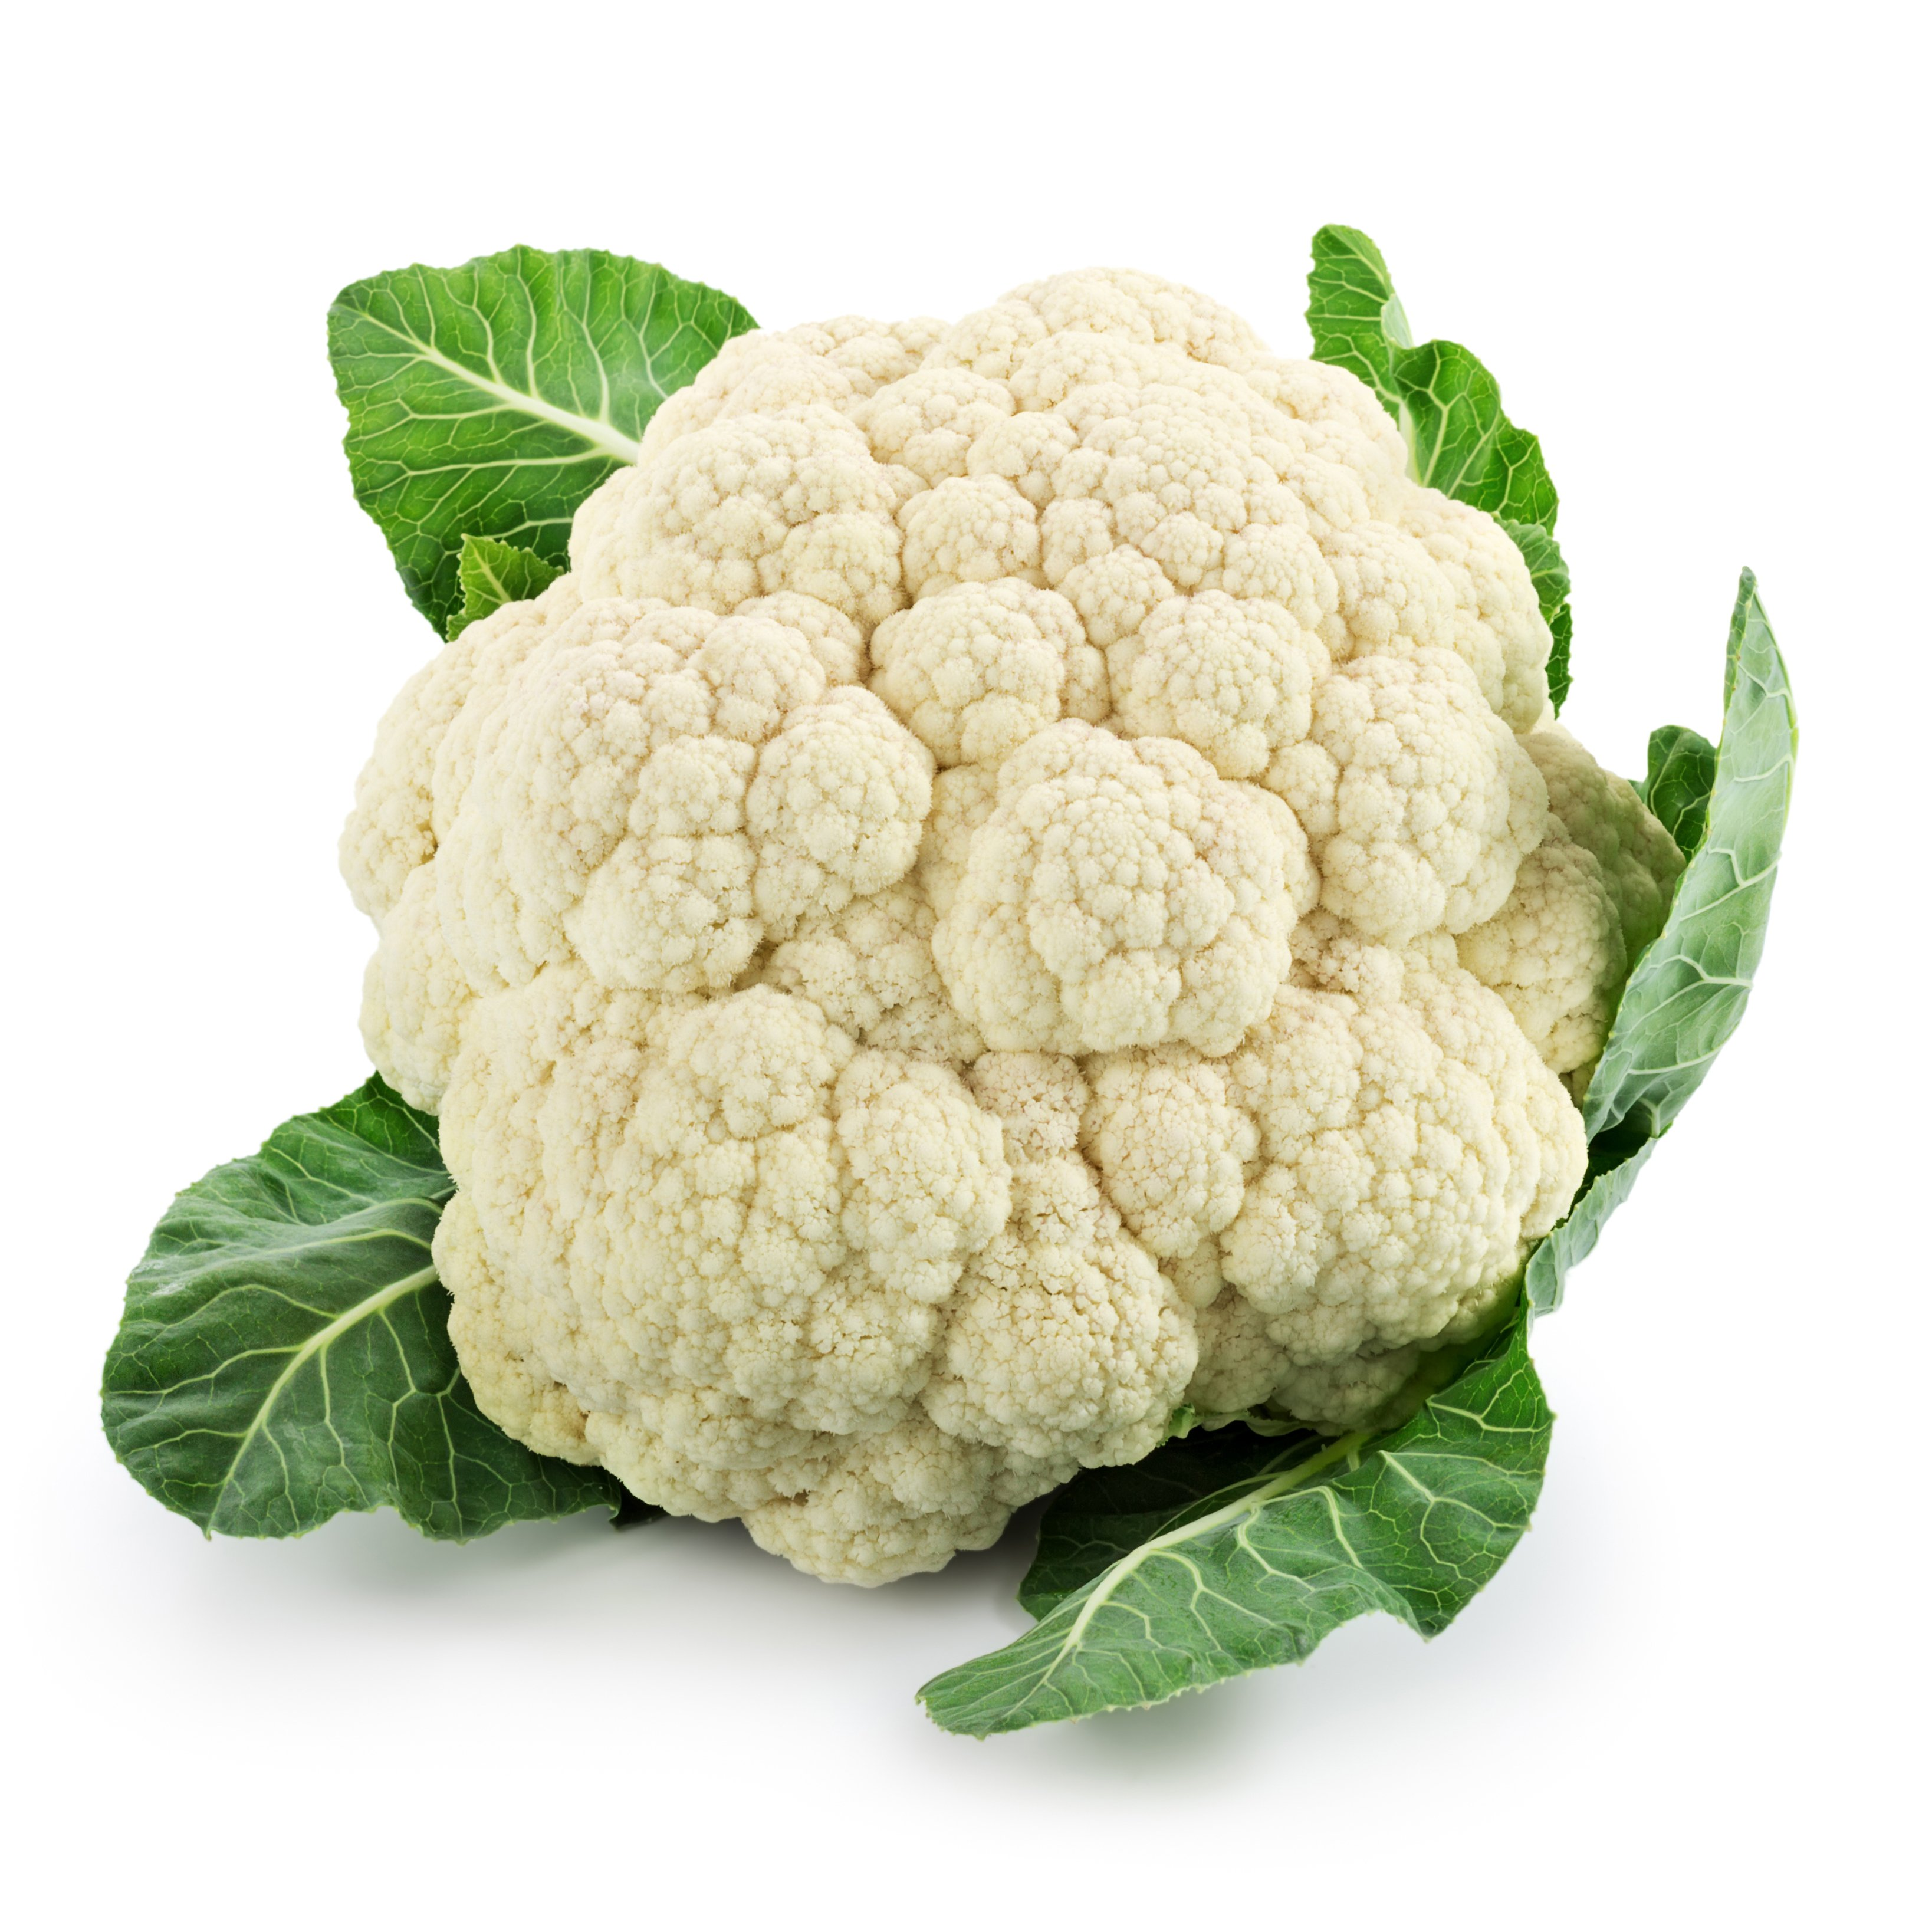
\includegraphics[width=7.5cm]{self-similarity/cauliflower.jpg}
			\caption{A cauliflower}
		\end{subfigure}
	%	\begin{subfigure}{.5\textwidth}
	%		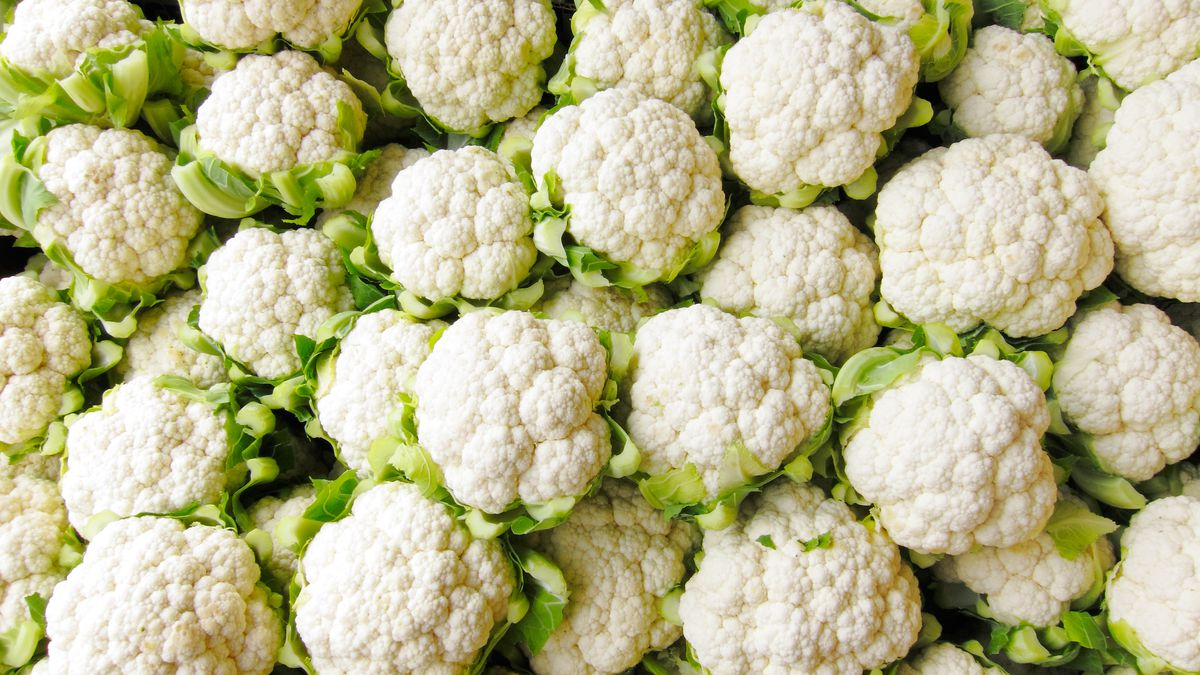
\includegraphics[width=.5\linewidth]{self-similarity/cauliflower_many.jpg}
	%		\caption{Many cauliflower}
	%	\end{subfigure}
		\begin{subfigure}[t]{.45\textwidth}
			\centering
			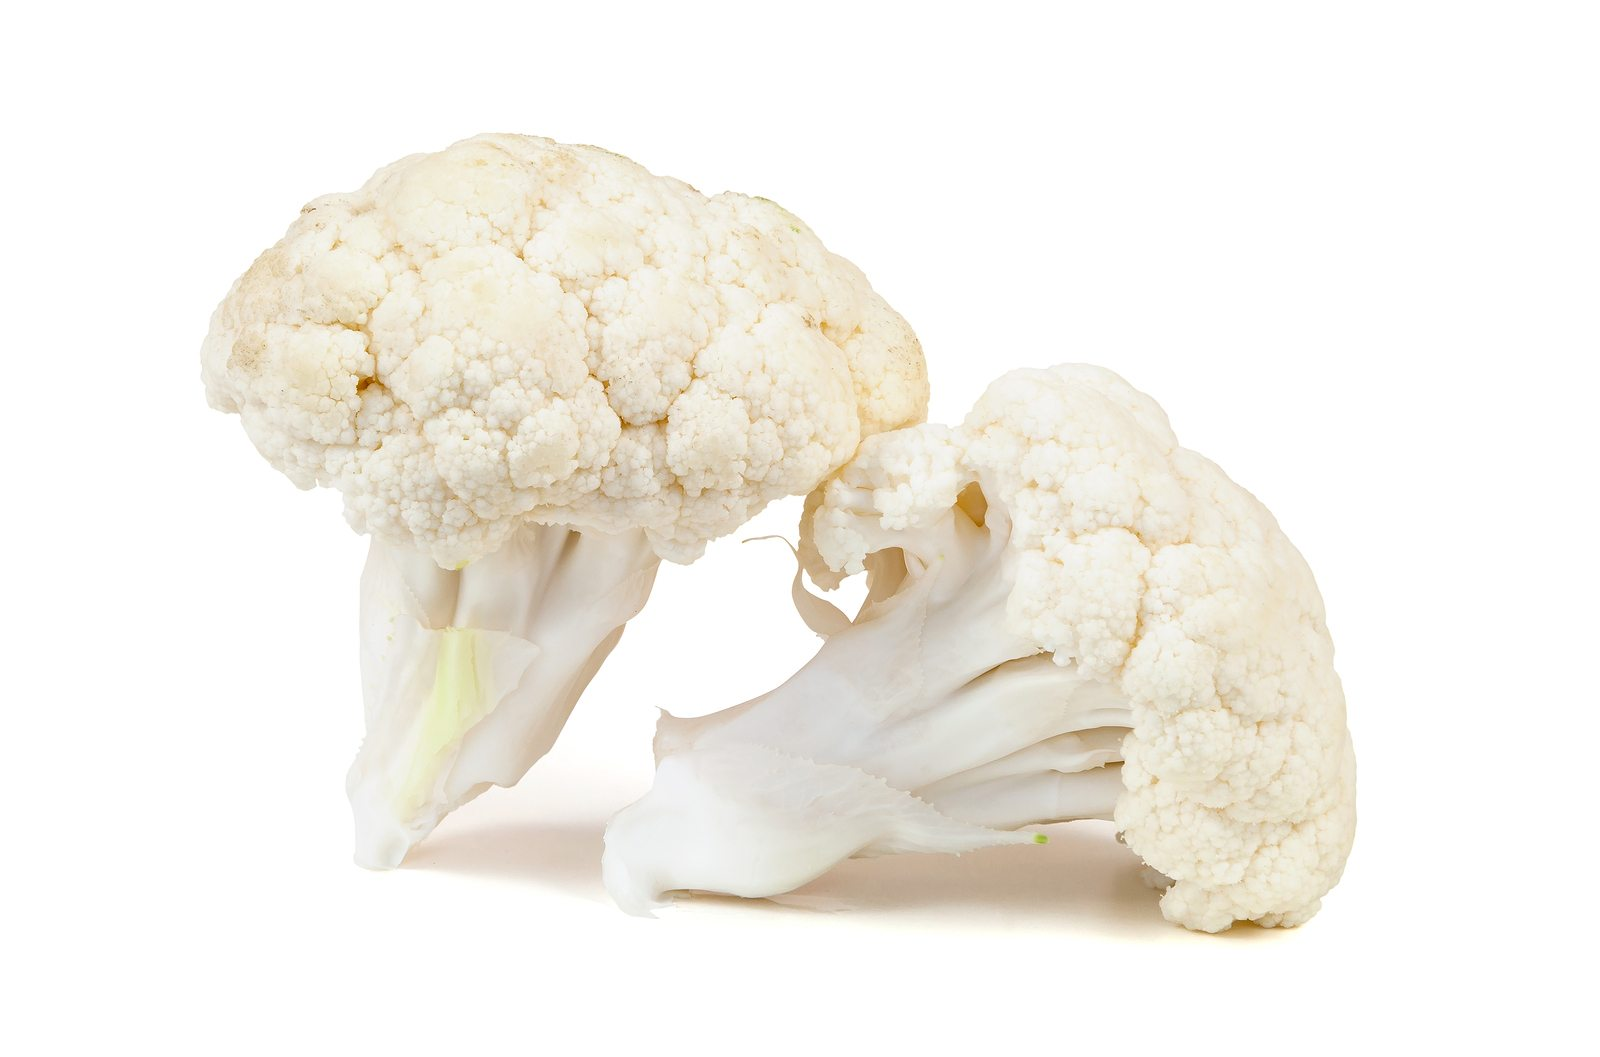
\includegraphics[width=7.5cm]{self-similarity/cauliflower_disected}
			\caption{Disection of cauliflower}
		\end{subfigure}
		\caption{Self-Similarity in Cauliflower}
		\label{fig:cauliflower-self-similarity}
	\end{figure}
	
	The cauliflower head contains branches or parts, which	when removed and compared with the whole found to be very much	the same except it is scaled down. These isolated branches can again	be decomposed into smaller parts, which again look very similar to the	whole as well as of the branches. Such self-similarity can easily be carried through for about three to four stages. After that the structures are	too small to go for further dissection. Of course, from the mathematical	point of view the property of self-similarity may be continued through	an infinite stages though in real world such property sustain only a few	stages \ref{fig:cauliflower-self-similarity}.
	
	\begin{figure}
		\centering
		\begin{tabular}{cc}
			% Requires \usepackage{graphicx}
			\begin{subfigure}{.6\textwidth}
				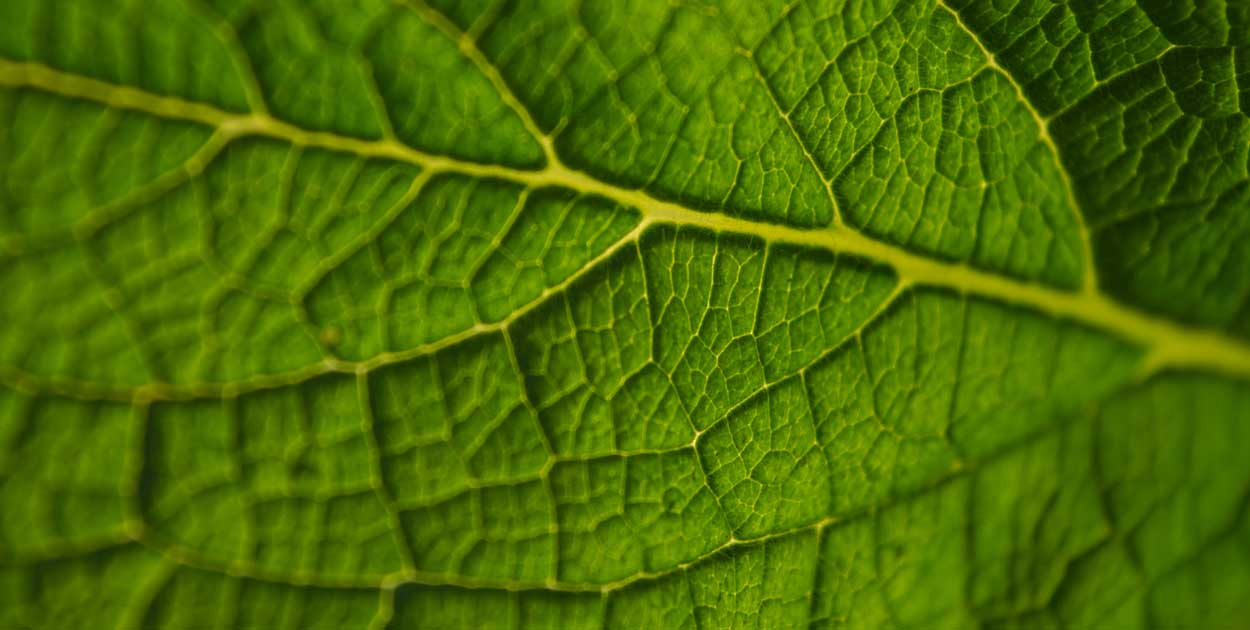
\includegraphics[width=60mm,height=50mm]{self-similarity/leaf.jpg}
				\caption{Leaf}		
			\end{subfigure}
			&
			\begin{subfigure}{.6\textwidth}
				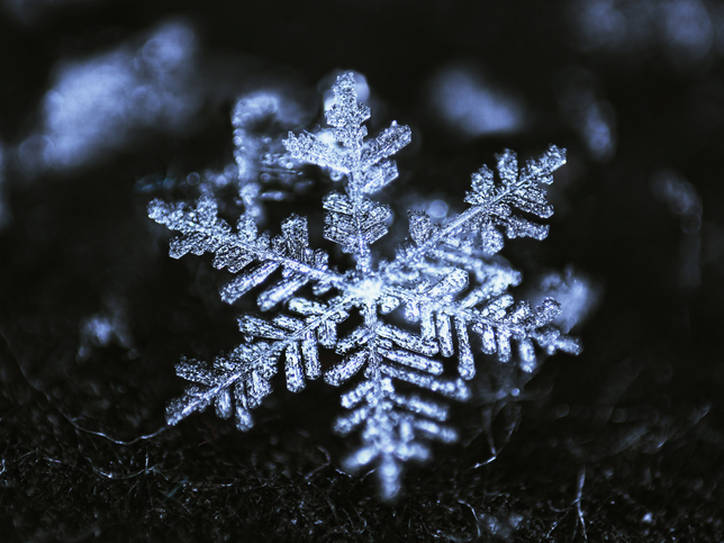
\includegraphics[width=60mm,height=50mm]{self-similarity/snowflake.jpg}
				\caption{Snowflake}		
			\end{subfigure}
			\\
			\begin{subfigure}{.6\textwidth}
				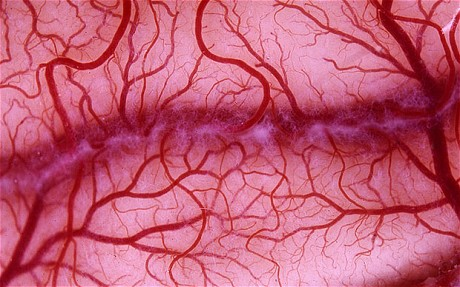
\includegraphics[width=60mm,height=50mm]{self-similarity/Blood_vessels.jpg}
				\caption{Blood vessel}		
			\end{subfigure}
			&
			\begin{subfigure}{.6\textwidth}
				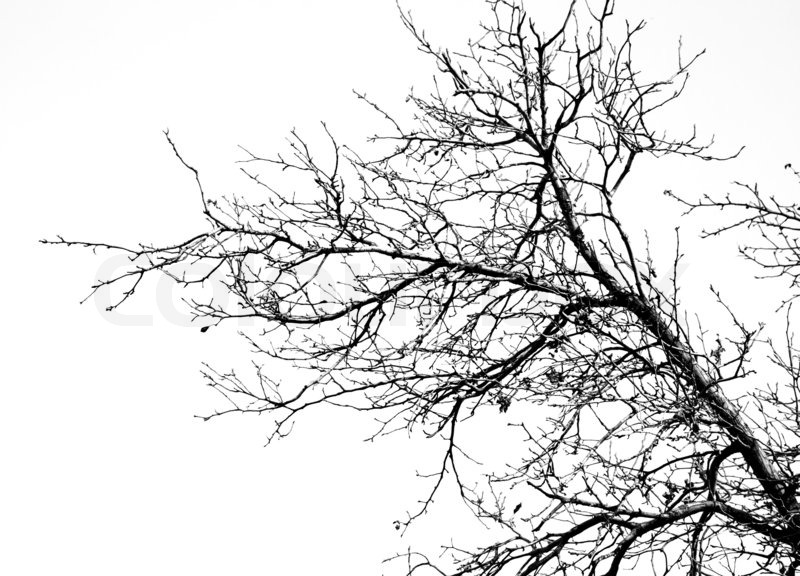
\includegraphics[width=60mm,height=50mm]{self-similarity/leafless-tree.jpg}
				\caption{Leafless Tree}		
			\end{subfigure}
			\\
		\end{tabular}
		
		\caption{Self-Similarity examples}
		\label{fig:example-self-similarity}
	\end{figure}


	There are plenty of other examples of self similarity in nature. Snowflakes exhibit self-similar branching patterns \ref{fig:example-self-similarity}. The growth in aggregating colloidal particles are statistically self-similar. A leafless tree branches \ref{fig:example-self-similarity} in a self-similar fashion, each length splitting into two or more branches. This branch pattern is repeated on smaller and smaller length scales till the tree top is reached. The veins of the leaves also branch in a self similar manner \ref{fig:example-self-similarity}. The decimal number system is a construct that uses the idea of self-similarity. If we look a meter stick, we shall see that a decimeter range with its marks looks like a meter range with its marks, only smaller by a factor of 10. This pattern of meter stick makes it very easy to note readings. The human brain is also a complex network of neurons which organize in self-similar patterns. From quantum particle paths, lightning bolts, blood vessels \ref{fig:example-self-similarity}, aggregation of bacteria all are example of self-similarity.
	
	One thing must be mentioned although it is understandable from the above discussion is that a system is to be called self-similar in the statistical sense even if it is not visible to the eye \cite{Mandelbrot1967}.
	
	
	
\section{Scaling Hypothesis}
	\subsection{Dynamic Scaling}
	Dynamic scaling (sometimes known as Family-Vicsek scaling \cite{Family1985, Vicsek1984}) is the litmus test of showing that an evolving system exhibits self-similarity.	A function $f(x,t)$ is said to obey dynamic scaling if one of the variable $t$ strictly denotes time and if it satisfies
	\begin{equation}
		f(x,t) \sim t^\theta \phi(x/t^z)
		\label{dynamic scaling definition}
	\end{equation}
	where $t$ is independent variable and $\theta$ and $z$ are fixed by the dimensional relation $\left[t^\theta\right] = \left[f\right]$ and $\left[t^z\right] = \left[x\right]$ respectively, while $\phi(\xi)$ is known as the scaling function. Sometimes it is also written in the following form
	\begin{equation}
	f(x,t) \sim x^\omega \phi(x/t^z)
	\label{dynamic scaling definition 2}
	\end{equation}
	where $x$ is consider independent variable.
	
	Buckingham $\pi$-theorem can provide a systematic processing procedure to obtain the dynamic scaling form and at the same time appreciate the fact that the second form is not mathematically sound. An interesting aspect of the structure of the dynamic scaling form given by equation \ref{dynamic scaling definition} is that the distribution function $f(x,t)$ at various moments of time can be obtained from one another by a similarity transformation
	\begin{align}
		x \rightarrow \lambda^z x \\
		t \rightarrow \lambda t \\
		f \rightarrow \lambda^\theta
	\end{align}
	revealing the self-similar nature of the function $f(x,t)$.\\
	
	To derive it one has to know first that one of the two governing parameters can be assumed to be independent. Let us assume that $t$ is	chosen to be an independent parameter and hence $x$ can be expressed	in terms of $t$
	\begin{equation}
	x \sim t^z
	\end{equation}
	It implies that we can choose $t^z$ as unit of measurement or yard-stick and quantify $x$ in terms of dimensionless quantity $\xi=x/t^z$. Here, the	quantity $\xi$ is a number that tells how many $t^z$ we need to measure $x$.	If $t$ is independent quantity then we can also express $f$ in units of $t^\theta$	to obtain yet another dimensionless quantity $\phi = f (x, t)/t^\theta$ where the	exponent $\theta$ is fixed by the dimensional requirement $\left[f\right] = \left[t^\theta\right]$. Since $\phi$ is a dimensionless quantity its numerical value can only depend on dimensionless quantity $\xi$ not on a dimensional quantity $t$. We	can then immediately obtain the scaling form given by Eq. \ref{dynamic scaling definition}. On	the other hand, had we choose $x$ to be independent parameter instead of	$t$ then following the same argument we would have the following scaling \ref{dynamic scaling definition 2}.
	
	
	\subsection{Finite Size Scaling}
	\label{subsect:FSS}
	Finite-size scaling, as formulated by Fisher and Barber \cite{Fisher1972}	concerns itself with the manner in which this rounding or crossover occurs. In a finite-size	system, there are in principle three length scales involved: $\xi, L$ and the microscopic length $a$	which governs the range of the interactions. Thermodynamic quantities thus may in principle	depend on the dimensionless ratios $\xi/a$ and $L/a$. The finite-size scaling hypothesis assumes	that, close to the critical point, the microscopic length drops out. Thus, if we consider a	quantity such as the ferromagnetic susceptibility $\chi$, which behaves like $ $ near the critical	point in the infinite system, then in the finite geometry characterized by a size $L$,
	\begin{equation}
		\chi = \chi^{\gamma/\nu} \phi(\xi/L)
	\end{equation}
	Equation of this sorts is used in any phase transition model.
	
	The finite-size scaling (FSS) \cite{Elsevier1988} has been extensively used as a very powerful tool for estimating finite size effects specially in the second order phase transition near the critical temperature $T$. The various response functions, typically the second derivative of the free energy $F$, in second order phase transition diverges. Such transitions are clasified by a set of critical exponents which characterize the critical point. The best known example of second order phase transition is the paramagnetic to ferromagnetic transition where
	\begin{align}
		M \sim (T-T_c)^\beta \\
		\chi_M \sim (T-T_c)^{-\gamma} \\
		C_V \sim (T-T_c)^{-\alpha} \\
		\xi \sim (T-T_c)^{-\nu}
	\end{align}
	where, $M, \chi_M, C_V, \xi$ are Magnetization, Susceptibility, Heat capacity, Correlation length respectively. These relations are only true in the thermodynamic limit in the sense that the system size is infinite. However, we can work in simulation and experiment with finite size $L^d$ where correlation length $\xi \sim L$. Finite size scaling thus provides a means of extrapolating various results for infinite systems.
	
	According to finite size scaling (FSS) hypothesis, a function $f(\epsilon, L)$ with $\epsilon = T-T_c$ is said to obey finite size scaling if it can be expressed as 
	\begin{equation}
		f(\epsilon, L) \sim L^{-\omega/nu} \phi(\epsilon L^{1/\nu})
		\label{fss 1}
	\end{equation}
	However, using the Buckingham $\pi$-theorem we not only obtain the correct scaling form but we also gain a deeper insight into the problem as it provides a systematic processing procedure. For instance, as we know that the correlation length $\xi$ in the limit $L \rightarrow \infty$ diverges like $\xi \sim \epsilon^\nu$ near the critical point and it bear the dimension of length. We therefore can either choose $L$ as an independent parameter and measure $\xi$,i.e., $T-T_c$, in unit of $L$. Consequently we can measure $L$ in unit of $T-T_c$ assuming it as an independent parameter. Choosing the later case we can define a dimensionless quantity
	\begin{equation}
		\pi = \frac{L}{\xi} = L(T-T_c)^\nu
	\end{equation}
	and the corresponding dimensionless governing parameter is 
	\begin{equation}
		\Pi = \frac{f(\epsilon, L)}{\xi^\omega} = \phi(\pi)
	\end{equation}
	Following the argument of the $\pi$-theorem we can immediately write that
	\begin{equation}
		f(\epsilon, L) \sim (T-T_c)^{-\nu \omega} \phi(L(T-T_c)^\nu)
	\end{equation}
	On the other hand had we chosen $L$ as an independent parameter then the similar treatment would yield
	\begin{equation}
		f(\epsilon, L)  \sim L^\theta \phi(\{L(T-T_c)^\nu\}^{-1})
	\end{equation}
	Till to date neither of the two scaling forms obtained following $\pi$ theorem are in use in their strict form. Instead, what is done traditionally are as follows. The important point is that if $\pi = L/\xi$ is dimensionless then so is 
	\begin{equation}
		\pi^{1/\nu} = (L/\xi^{1/\nu}) = (T-T_c) L^{1/\nu}
	\end{equation}
	It also means that we can choose $L$ as independent parameter and express $(T-T_c)$ in unit of $L^{-1/\nu}$ to make the dimensionless quantity coincide with $\pi^{1/\nu}$. Then $f$ too can be expressed in unit of $L^\theta$ which according to the prescription of $\pi$-theorem we have the following FSS scaling form
	\begin{equation}
		f(\epsilon, L) \sim L^\theta \phi((T-T_c)L^{1/\nu})
	\end{equation}
	which is the same as the traditional scaling form given by \ref{fss 1} if we find $\theta$ negative and it is related to the exponent $\nu$ via $\theta=-\omega/\nu$.\\
	A quantitative way of interpreting how the experimental data exhibits finite-size scaling is done by invoking the idea of data-collapse method - an idea that goes back to the original observation of Rushbrooke. That is, the values of $f(\epsilon,L)$ for different system size $L$ can be	made to collapse on a single curve if $f L^{\omega/\nu}$ is plotted against $\epsilon L ^{1/\nu}$ . It	implies that systems of different sizes are all similar that also include	system where $L \rightarrow \infty$. The method of data-collapse therefore comes as	a powerful means of establishing scaling. It is extensively used to analyze and extract exponents especially from numerical simulations. We	shall elucidate it further in the upcoming chapters.
	
	
	
\section{Homogeneous Functions and Scale-Invariance}
	\label{sect:homogenious-function}
	In mathematics, a homogeneous function is one with multiplicative scaling behaviour: if all its arguments are multiplied by a factor, then its value is multiplied by some power of this factor.
	
	For example, a homogeneous function of two variables $x$ and $y$ is a real-valued function that satisfies the condition
	\begin{equation}
		f(\lambda x, \lambda y) = \lambda^k f(x,y)
	\end{equation} 
	 for some constant $k$ and all real numbers $\lambda$ . The constant  $k$ is called the degree of homogeneity \cite{Kluwer1994}.
	
	
	\subsection{One variable function}
	A function is called scale-invariant or scale-free if it retains its form keeping all its characteristic features intact even if we change the measurement unit or scale. Mathematically, a function $f(r)$ is called scale-invariant or scale-free if it satisfies
	\begin{equation}
		f(\lambda x) = g(\lambda) f(x) \ \forall \lambda
		\label{scale free eqn}
	\end{equation}
	where $g(\lambda)$ is yet unspecified function. That is, one is interested in the shape of $f(\lambda x)$ for some scale factor $\lambda$ which can be taken to be a length or size rescaling. For instance dimensional functions of physical quantity are always scale-free since they obey power monomial law. It can be rigorously proved that the function that satisfies \ref{scale free eqn} should always have power law of the form $f(x) \sim x^{-\alpha}$.\\
	Let us first set $r=1$ to obtain $f(\lambda) = g(\lambda)f(1)$. Thus $g(\lambda)=f(\lambda)/f(1)$ and equation \ref{scale free eqn} can be written as
	\begin{equation}
		f(\lambda x) = \frac{f(\lambda) f(x)}{f(1)}
	\end{equation}
	The above equation is supposed to be true for any $\lambda$, we can therefore differentiate both sides with respect to $\lambda$ to yield
	\begin{equation}
		x f^\prime(\lambda x) = \frac{f^\prime(\lambda) f(x)}{f(1)}
	\end{equation}
	where $f^\prime$ indicates the derivative of $f$ with respect to its argument. Now we set $\lambda=1$ and get
	\begin{equation}
		x f^\prime(x) = \frac{f^\prime(1) f(x)}{f(1)}
	\end{equation}
	This is a first order differential equation which has a solution
	\begin{equation}
		f(x) = f(1) x^{-\alpha}
	\end{equation}
	where $\alpha = - f(1) / f^\prime (1)$. There it is proven that the power law is the only solution that can satisfy \ref{scale free eqn}. We can also prove that $g(\lambda)$ has a power law form as well.\\
	Power law distribution of the form $f(x) \sim x^{-\alpha}$ are said to be scale free since the ratio $\frac{f(\lambda r)}{f(x)}$ depends on $\lambda$ alone. Thus the distribution does not need a characteristic scale. If we change the unit of measurement of $x$ by a factor of $\lambda$, the numerical value of $f(x)$ will change by a factor of $g(\lambda)$, without affecting the shape of the function $f$. 
	
	
	
	\subsection{Generalized Homogeneous Function}
	A function $f(x,y)$ of two independent variables $x$ and $y$ is said to be a generalized homogeneous function if for all values of the parameter $\lambda$ the function $f(x,y)$ satisfies,
	\begin{equation}
		f(\lambda^a x, \lambda^b y) = \lambda f(x,y)
		\label{generalized homogeneous function}
	\end{equation}
	where $a,b$ are arbitrary numbers. In contrast to the homogeneous functions defined in the previous section \ref{label} generalized homogeneous functions can not be written as $f(\lambda x, \lambda y) = \lambda^p f(x,y)$, because \ref{generalized homogeneous function} can not be generalized any further to the following form,
	\begin{equation}
		f(\lambda^a x, \lambda^b y) = \lambda^p f(x,y)
	\end{equation}
	choosing $p=1$ in the above equation yields
	\begin{equation}
		f(\lambda^{a/p} x, \lambda^{b/p} y) = \lambda f(x,y)
	\end{equation}
	Similarly an statement converse is also valid and the equation above is no more general than the form in the equation \ref{generalized homogeneous function}. Another equivalent form of \ref{generalized homogeneous function}  is as follows,
	\begin{equation}
		f(\lambda x, \lambda^b y) = \lambda^p f(x,y)
	\end{equation}
	Similarly
	\begin{equation}
		f(\lambda^a x, \lambda y) = \lambda^p f(x,y)
	\end{equation}
	Note that there are at least two undetermined parameters $a$ and $b$ for a generalized homogeneous function. Now let use see what happens if we choose $\lambda^a = 1/x$ to set in equation \ref{generalized homogeneous function},
	\begin{align}
		f(1, \frac{y}{x^{b/a}}) &= x^{-\frac{p}{a}} \\
		f(x,y) &= x^{p/a} f(y/x^{b/a})
	\end{align}
	This combining and hence the simplification of two variables $x$ and $y$ into a single term has far reaching consequence in Widom scaling \cite{Kleinert2001, Huang1987, Sabbir}in the theory of phase transition and critical phenomena. 
	
	
	In Statistical Mechanics we have a hypothesis called widom scaling (names after Benjamin Widom)  regarding the free energy of a magnetic system near its critical point which leads to the critical exponents. And becomes no longer independent so that they can be parameterized in terms of two values. The hypothesis can be seen to arise as a natural consequence of the block-spin renormalization procedure, when the block size is chosen to be of the same size as the correlation length \cite{Stanley1987, Kleinert2001, Huang1987}.	Widom scaling is an example of universality.
% Uncomment this line, when you have siunitx package loaded.

%!TEX root = ../thesis.tex
%*******************************************************************************
%****************************** Third Chapter **********************************
%*******************************************************************************
\chapter{Phase Transition}
\label{chapter.phase-transition}

% **************************** Define Graphics Path **************************
\ifpdf
    \graphicspath{{Chapter3/Figs/thermodynamics/}{Chapter3/Figs/}{Chapter3/Figs/ising-model/}}
\else
    \graphicspath{{Chapter3/Figs/thermodynamics/}{Chapter3/Figs/}{Chapter3/Figs/ising-model/}}
\fi

The term phase transition is generally use to describe the transition between solid, liquid or gaseous states and in some cases the plasma state. It is one of the most studied problem in physics. Phase transition is a process where below a critical point the system behaves in one way whereas above that point the system behaves in a completely different way. There is a control parameter in phase transition. It can be temperature $T$ or magnetic field $H$. For example in ferromagnet to paramagnet transition temperature is the control parameter and for normal to superconductor transition both temperature and magnetic field are the control parameter.


\section{Classification}
	\subsection{Ehrenfest classification}
	Paul Ehrenfest classified phase transitions based on the behavior of the thermodynamic free energy as a function of other thermodynamic variables \cite{Jaeger1998}. Under this scheme, phase transitions were labeled by the lowest derivative of the free energy that is discontinuous at the transition. 
	
	First-order phase transitions exhibit a discontinuity in the first derivative of the free energy with respect to some thermodynamic variable \cite{Blundell2006}. The various solid/liquid/gas transitions are classified as first-order transitions because they involve a discontinuous change in density, which is the (inverse of the) first derivative of the free energy with respect to pressure. 
	
	Second-order phase transitions are continuous in the first derivative (the order parameter, which is the first derivative of the free energy with respect to the external field, is continuous across the transition) but exhibit discontinuity in a second derivative of the free energy \cite{Blundell2006}. These include the ferromagnetic phase transition in materials such as iron, where the magnetization, which is the first derivative of the free energy with respect to the applied magnetic field strength, increases continuously from zero as the temperature is lowered below the Curie temperature. The magnetic susceptibility, the second derivative of the free energy with the field, changes discontinuously. Under the Ehrenfest classification scheme, there could in principle be third, fourth, and higher-order phase transitions.
	
	Though useful, Ehrenfest's classification has been found to be an incomplete method of classifying phase transitions, for it does not take into account the case where a derivative of free energy diverges (which is only possible in the thermodynamic limit). For instance, in the ferromagnetic transition, the heat capacity diverges to infinity. The same phenomenon is also seen in superconducting phase transition.
	
	\subsection{Modern classifications}
	In the modern classification scheme, phase transitions are divided into two broad categories, named similarly to the Ehrenfest classes:\cite{Jaeger1998}
	
	First-order phase transitions are those that involve a latent heat. During such a transition, a system either absorbs or releases a fixed (and typically large) amount of energy per volume. During this process, the temperature of the system will stay constant as heat is added: the system is in a "mixed-phase regime" in which some parts of the system have completed the transition and others have not. Familiar examples are the melting of ice or the boiling of water (the water does not instantly turn into vapor, but forms a turbulent mixture of liquid water and vapor bubbles). 
	
	Second-order phase transitions are also called continuous phase transitions. They are characterized by a divergent susceptibility, an infinite correlation length, and a power-law decay of correlations near criticality. Examples of second-order phase transitions are the ferromagnetic transition, superconducting transition (for a Type-I superconductor the phase transition is second-order at zero external field and for a Type-II superconductor the phase transition is second-order for both normal-state—mixed-state and mixed-state—superconducting-state transitions) and the superfluid transition. In contrast to viscosity, thermal expansion and heat capacity of amorphous materials show a relatively sudden change at the glass transition temperature \cite{Ojovan2013} which enables accurate detection using differential scanning calorimetry measurements
	
	\subsection{Basic Properties of the classes}
	Some basic properties of the two classes of phase transition is listed below.
	\paragraph{First Order}
		\begin{enumerate}
			\item Latent heat of nucleation in growth
			\item Symmetry may or may not be broken
			\item Discontinuous change in entropy
		\end{enumerate}
	
	\paragraph{Second Order}
		\begin{enumerate}
			\item No Latent heat or meta-stable state
			\item Sysmmetry is always broken
			\item Continuous change in entropy
		\end{enumerate}
	At the event of critical point of phase transition there might exists a meta-stable state, where both phases exists simultaneously. At the meta-stable state the control parameter or temperature (in case of thermal phase transition, e.g., ice to water or water to vapor) does not change but there is a change (usually large) in heat which give rise to discontinuity of the first derivative of free energy, i.e., entropy (\ref{subsect:entropy-thermodynamics}, \ref{subsect:percolation-entropy}). And if the entropy is continuous then the latent heat is zero which is the signature of second order transition.

	
	
\section{Thermodynamic Quantities}
	The first explicit statement of the first law of thermodynamics, by \textit{Rudolf Clausius} in 1850, referred to cyclic thermodynamic processes.
	
	
	\textit{In all cases in which work is produced by the agency of heat, a quantity of heat is consumed which is proportional to the work done; and conversely, by the expenditure of an equal quantity of work an equal quantity of heat is produced.}
	
	\begin{align}
		\Delta E = Q + W
	\end{align}
	where, $Q$ is the net quantity of heat supplied to the system by its surroundings and $W$ is the net work done by the system.
	The IUPAC convention for the sign is as follows: All net energy transferred to the system is positive and net energy transferred from the system is negative.
	Clausius also stated the law in another form, referring to the existence of a function of state of the system, the internal energy, and expressed it in terms of a differential equation for the increments of a thermodynamic process.
	
	\textit{In a thermodynamic process involving a closed system, the increment in the internal energy is equal to the difference between the heat accumulated by the system and the work done by it.}
	
	For quasi-static process
	\begin{align}
		dU &= \delta Q - \delta W \label{def:enternal-energy}\\
		  &= dQ - P dV
	\end{align}
	$U$ is the internal energy.
	here $W = -P dV$
	since work done by the system on the environment if the product $P dV$ whereas the work done on the system is $-P dV$ for pressure $P$ and volume change $dV$.\\
	The term heat for $Q$ means "that  amount of energy added or removed by conduction of heat or by thermal radiation", rather than referring to a form of energy within the system. 
	The internal energy is a mathematical abstraction that keeps account of the exchanges of energy that befall the system.
	
	For quasi-static state we can write
	\begin{equation}
	dQ = T dS
	\label{eqn:def_enthalpy}
	\end{equation}
	where $S$ is the entropy of the system and $T$ is the temperature.
	Thus we can write for canonical ensemble
	\begin{equation}
	dU = TdS - PdV
	\label{def:internal-energy--entropy-volumn}
	\end{equation}
	such that $E=E(S,V)$  and 
	for grand canonical ensemble 
	\begin{equation}
	dU = TdS - pdV + \mu dN
	\end{equation}
	where $U=U(S,V,N)$.
	But a problem arises, since there is no device we currently posses that can measure entropy. So we use Legendre transformation to change variable dependency
	\begin{align}
		dU  	&= TdS - pdV  \nonumber \\ 
		&= TdS + SdT - SdT - PdV  \nonumber \\ 
		d(U-TS) &= -SdT - PdV  \nonumber \\
		dA 		&= -SdT - PdV \label{eqn:helmholtz_def}
	\end{align}
	where $A=A(T,V)$  is the Helmholtz free energy. We can perform another Legendre transformation in (\ref{eqn:helmholtz_def}) as follows
	\begin{align}
		dA 		&= -SdT - PdV -VdP + VdP \nonumber \\
		d(A+PV) &= -SdT + VdP \nonumber \\
		dG      &= -SdT + VdP \label{eqn:gibbs_def}
	\end{align}
	where $G=G(T,P)$ is the Gibbs free energy.
	
	
	\subsection{Entropy}
	\label{subsect:entropy-thermodynamics}
	One of the most important concept in Statistical Mechanics is entropy. The notion of entropy was first introduced in physics by a German scientist Rudolf Clausius who laid the foundation for the second law of thermodynamics in 1850 by examining the relation between heat transfer and work.
	The second law of thermodynamics states that the total entropy of an isolated system can never decrease over time. Therefore the direction toward which entropy increases monotonically is the direction of time. Monotonically means that it can increase or keep constant but never decrease.	The term entropy	is used in many other branches of science, sometimes distant from physics or mathematics (such	as sociology), where it no longer maintains its rigorous quantitative character. Usually, it roughly	means disorder, chaos, decay of diversity or tendency toward uniform distribution of kinds \cite{Downarowicz2009}.
	
	
	
	Entropy is considered as a quantity about the disorderness of a system. This kind of disorder is the number of states a system can take on. So what are the states of a system? Imagine a cube of volume $1cm^3$, filled with one particular gas. At a particular time if we can label all the molecules of the gas uniquely then at next moment most of the molecule will change their positions due to their random motion. Then we will not be able to identify each molecule with their previous label. This process of identifying the labels of the molecules are easier if it's a liquid and even more easier in it's solid form. Since temperature increases the random motion of the molecules, as the temprature rises it is more difficult to identify those molecules. Thus at high temperature a system has higher entropy. Another thing to mention about it's volume. If a larger volume is selected then obviously the number of possible states will increase therefore entropy will increase.
	
	
	\paragraph{Example}
	If we were ot compare the entropy of the moon and the sun, the above discussion tells us that the sun has higher entropy than the moon. The reason is that the sun is much much larger than the moon and has much higher temperature than the moon. Therefor the number of possible states will be larger for the sun than the moon.
	
	
	In Classical Physics, entropy is seen as a magnitude which in every time is proportional to	the quantity of energy that at that time cannot be transformed into mechanical work. Using the	above interpretation, entropy plays a central role in the formulation of the second law of thermodynamics which states that in an isolated physical system, any transformation leads to an increase	of its entropy. 
	
	In Probability Theory, the entropy of a random variable measures the uncertainty over the	values which can be reached by the variable.
	
	In Information Theory, the entropy of the compression of a message (for example, of a file	from a computer), quantifies the content of the information of the message to have the minimum	lost of information in the compression process previous to its transmission.
	
	In Abstract Theory of Dynamical Systems, the entropy measures the exponential complexity	of the system or the average flow of information per unit of time \cite{Balibrea2016}.
	
	So it is already explicit that the concept of entropy is not easy to grasp and frequently entropy is seen as very mysterious quantity and that’s why it received a very large number of interpretations,
	explications, applications. In order to understand how the complex concept of entropy emerged,
	in this chapter we will give a brief history and will review the works of Clausius, Boltzmann,
	Shannon and R\'{e}nyi.

	\subsubsection{Clausius Entropy}	
	As mentioned Earlier in this section The concept and name of entropy originated in the early 1850s in the work of Rudolf Julius Emmanuel Clausius $(1822-1888)$ and that work was at first	primarily concerned with the question of which cycle is best suited for the conversion of heat into	work and which substance is best used for the conversion \cite{Clausius1867}.
		
	Clausius based his argument on the plausible axiom that heat cannot pass by itself from a cold to a hot body. In order to exploit that axiom Clausius considered two competing Carnot cycles (see figure	(\ref{fig:carnot-engines})) working in the same temperature range, one as a heat engine and one as a refrigerator;	the refrigerator consumes the work the engine provides. By comparing the amounts of heat $Q$	passed from top to bottom and vice versa, he came to the conclusion that among all efficiencies	the efficiency of a Carnot cycle is maximum and universal.	'Maximum' means that no cycle in the same range of temperature has a bigger efficiency than a	Carnot cycle, and 'universal' means that all working substances provide the same efficiency in a	Carnot cycle \cite{Carnot1890}.	It is easy to calculate the efficiency of the Carnot engine of an ideal gas:
	\begin{figure}
		\centering
		\includegraphics[width=10cm]{{{carnot-cycle-heat-engine-refrigerator}}}
		\caption{Two competing Carnot engines, pressure (P) versus volume (V) - diagrams \cite{Greven2003}}
		\label{fig:carnot-engines}
	\end{figure}
	\begin{align}
		\eta &= \frac{W}{Q_{boiler}} \nonumber\\
 			 &= \frac{Q_{boiler} - Q_{cooler}}{Q_{boiler}} \nonumber\\
 			 &= 1 - \frac{Q_{cooler}}{Q_{boiler}} \\
 			 &= 1 - \frac{T_{cooler}}{T_{boiler}}
 	\label{eqn:efficiency-carnot}
	\end{align}
	where $T$ is the Kelvin temperature. And, since by Clausius’s result this efficiency is universal, it	holds not only for ideal gases but for all substances, be they water, mercury, sulphur, or steel.
	Nicolas L\'{e}onard Sadi Carnot anticipated Clausius by 30 years, but no one could understand	Carnot's reasoning. Carnot believed in the caloric theory of heat, by which the heat passing through	the cycle from boiler to cooler is unchanged in amount. This is quite wrong and it is a kind of miracle that Carnot, despite his erroneous concepts, obtained a correct result. Carnot's trouble was	that he did not know the balance of energy, or the first law of thermodynamics, which states that
	\begin{align}
		dU &= dQ - dW \\
  		   &= dQ - P dV
	\end{align}
	since
	\begin{equation}
		dW = P dV
	\end{equation}
	This equation holds, if the work is expended reversibly for the volume change. With that superior	knowledge Clausius showed that it is not the heat that passes through the cycle from boiler to	cooler unchanged in amount. He proved that from equation (\ref{eqn:efficiency-carnot})
	\begin{equation}
		\frac{Q}{T}\at[\Big]{\text{boiler}} =
		\frac{Q}{T}\at[\Big]{\text{heater}}
	\end{equation}
	nd decided to define the entropy change to be the ratio of heat flow to temperature: \cite{Sethna2006}
	\begin{equation}
		\Delta S_{\text{thermo}} = \frac{Q}{T}
	\end{equation}
	He also showed that in an arbitrary process, the change of entropy, satisfies the inequality
	\begin{equation}
		dS \geq \frac{dQ}{T}
		\label{eqn:2nd-law-of-themodynamics}
	\end{equation}
	This important relation is known as the second law of thermodynamics. We will now discuss the significance of this law.
	First, we stick to reversible process, where the equality holds in equation (\ref{eqn:2nd-law-of-themodynamics}). We may then eliminate $dQ$ between the first and second laws, we obtain the Gibbs equation
	\begin{equation}
		dS = \frac{1}{T} \left(dU + P dV\right)
	\end{equation}
	In an adiabatic irreversible process, $dQ = 0$ and equation (\ref{eqn:2nd-law-of-themodynamics}) one has the fundamental relation between entropy and irresponsibility. In words
	
	\textbf{In a closed system (adiabatic), the entropy cannot decrease, it remains constant or increase \cite{Benguigui2013}}
		
	But the irreversible increase of entropy is not a property of the microscopic laws of nature. Because the microscopic laws of nature are time-reversal invariant. For example the Maxwell's equations are time reversible or the laws governing the motion of electrons of atoms are also time reversible. Thus the direction of time cannot be determined from microscopic laws of nature. But since entropy always increase monotonically, the direction in which entropy increases (or remains constant) is the direction of time \cite{Sethna2006}.
	
	
	Also by differentiating equation (\ref{eqn:gibbs_def}) with respect to $T$ keeping $P$ constant we can get an expression for entropy in terms of the Gibbs free energy.
	\begin{equation}
		S = -\frac{dG}{dT}
	\end{equation}
	similar expression is obtained from (\ref{eqn:helmholtz_def}). Thus entropy is indeed the first derivative of free energy with respect to the control parameter $T$.
	
	
	%----------------------------------------------
		\subsubsection{Boltzmann Entropy}
		Another intuitive interpretation of entropy is as a measure of the disorder in a system.  Liquids have higher entropy	than crystals intuitively because their atomic positions are less orderly \cite{Sethna2006}. Ludwig Boltzmann	interpreted the entropy function as statistical entropy using probability theory.	Around 1900 there was a fierce debate going on between scientists whether atoms really existed	or not. Boltzmann was convinced that they existed and realized that models that relied on atoms	and molecules and their energy distribution and their speed and momentum, could be of great	help to understand physical phenomena. Because atoms where supposed to be very small, even	in relatively small systems, one faces already a tremendous number of atoms. For example: one
		mole of water contains about $6.023 \times 10^{23}$ molecules! Clearly it is impossible to track the energy	and velocity of each individual atom. Therefore, Boltzmann introduced a mathematical treatment	using statistical mechanical methods to describe the properties of a given physical system (for example the relationship between temperature, pressure and volume of one liter of air). 
		
		Boltzmann's	idea behind statistical mechanics was to describe the properties of matter from the mechanical	properties of atoms or molecules. In doing so, he was finally able to derive the Second Law of	Thermodynamics around 1890 and showed the relationship between the atomic properties and the	value of the entropy for a given system. It was Max Planck who formulated the expression of entropy of the ideal gas system based on Boltzmann’s results \cite{Schmitz2007}. The Boltzmann entropy formula	or Boltzmann-Planck entropy formula is
		\begin{equation}
			S = k_B \log\Omega
			\label{eqn:boltzmann-entropy}
		\end{equation}
	
		$S$ is called the Planck entropy or Boltzmann entropy. Here $k_B$ is the Boltzmann constant
		(ideal gas constant $R$ divided by Avogadro's number $N$) which equals to $1.4 \times 10^{-23}$ $J/K$), and $\Omega$, comes from the German \textit{Wahrscheinlichkeit}, meaning probability, which is often referred to as	disorder. In another way we can define it as the number of microstates (often modeled as quantum	states) with the given macrostate. Macrostate is any particular arrangement of atoms where we	look only on average quantities. Any individual arrangement defining the properties (e.g. positions	and velocities) of all the atoms for a given macrostate is a microstate. For a microstate it matters	what individual particles do, for the macrostate it does not.
		
		
		The logarithm is used because it simplifies the computations and reproduced the property of additivity of entropy, in the sense that the entropy of two systems sums instead of multiplies. In	equation (\ref{eqn:boltzmann-entropy}), the entropy $S$ increases when $\Omega$ increases. More microstates give raise to more disorder	hence higher entropy. Besides for only one possible microstate, entropy is zero. The notion of	disorder is an intuitive notion depending of the system to be considered. In the case of a gas, it	is considered it in a ordered state if its molecules have a distribution of energies or positions very	
		different of those random which means the Boltzmann distribution. The most disordered states are	the most probable and as consequence have the most entropy. Another consequence is that in the	universe the disorder tends to increase \cite{Balibrea2016}.
		
		
		From there, it is a short conceptual jump to the second Law (total entropy tends to increase, and	all spontaneous processes increase entropy). In summary, the thermodynamic definition of entropy provides the experimental definition of entropy, while the probabilistic definition of entropy	extends the concept, providing an explanation and a deeper understanding of its nature \cite{Alam2016}.
		
		These definitions of entropy is of no use in our model. However we can use the Boltzmann entropy with a few modification to get Shannon entropy \cite{Shannon1948}. This process of getting Shannon entropy from Boltzmann entropy and how does it help us is described in section (\ref{subsect:percolation-entropy}).

	
	\subsection{Specific Heat}
	Heat capacity is a physical quantity which is the ratio of the heat added to an object to the resulting temperature change \cite{Walker2013}. Note that removing heat is just like adding negative heat. The unit of heat capacity if joule per kelvin $j/K$. And it's dimensional form is $L^2MT^{-2}\Theta^-1$.	The specific heat is the amount of heat per unit mass ($1kg$) required to raise the temperature by one kelvin($1K$). 
	
	
	Heat capacity is an \textit{extensive} property of matter (it is proportional to the size of the system). When expressing the same phenomenon as an \textit{intensive} property, the heat capacity is divided by the amount of substance, mass, or volume, thus the quantity is independent of the size or extent of the sample. The molar heat capacity is the heat capacity per unit amount (SI unit: mole) of a pure substance, and the specific heat capacity, often called simply specific heat, is the heat capacity per unit mass of a material. In some engineering contexts, the volumetric heat capacity is used.
	
	Temperature represents the average randomized kinetic energy of constituent particles of matter relative to the centre of mass of the system, while heat is the transfer of energy across a system boundary into the body other than by work or matter transfer. Translation, rotation, and vibration of atoms represent the degrees of freedom of motion which classically contribute to the heat capacity of gases, while only vibrations are needed to describe the heat capacities of most solids, as shown by the Dulong–Petit law \cite{Kittel2004}.
	
	
	The internal energy of a closed system changes by adding heat to the system or by the system performing work.
	\begin{equation}
		\Delta E_{system} = E_{in} - E_{out}
	\end{equation}
	which is same expression as (\ref{def:enternal-energy}). If the heat is added at constant volume, then the second term of this relation vanishes to give
	\begin{equation}
		C_V = \left(\frac{\partial U}{\partial T}\right)_V = \left(\frac{\partial Q}{\partial T}\right)_V
	\end{equation}
	Another useful quantity is the heat capacity at constant pressure, $C_P$. This quantity refers to the change in the enthalpy of the system given by
	\begin{equation}
		H = U + PV
	\end{equation}
	Thus the change in enthalpy is 
	\begin{align}
		dH 
		&= dU + d(PV) \nonumber \\
		&= dQ + dW + PdV + VdP \nonumber \\
		&= dQ  + VdP
	\end{align}
	Therefore at constant pressure we have
	\begin{equation}
		C_P = \left(\frac{\partial H}{\partial T}\right)_P = \left(\frac{\partial Q}{\partial T}\right)_P
	\end{equation}
	In general we can write the relationship between heat and temperature change as
	\begin{equation}
		C = \frac{Q}{dT}
	\end{equation}
	 where $C$ is the specific heat.
	and we know
	\begin{equation}
		Q = T dS
	\end{equation}
	we immediately get
	\begin{equation}
		C = T \frac{dS}{dT}
		\label{def:specific-heat-thermodynamics}
	\end{equation}
	Specific heat is called the response function for a non-magnetic system.
		
		
	\subsection{Order Parameter}
	An order parameter is a measure of the degree of order across the boundaries in a phase transition system. It's numerical usually ranges between $[0,1]$. At the critical point, the order parameter susceptibility will usually diverge.
	
	An example of an order parameter is the net magnetization in a ferromagnetic system undergoing a phase transition. For liquid-gas transitions, the order parameter is the difference of the densities.
	
	Order parameter does have a theoretical perspective. It arise from symmetry breaking. When this happens, one needs to introduce one or more extra variables to describe the state of the system. For example, in the ferromagnetic phase, one must provide the net magnetization, whose direction was spontaneously chosen when the system cooled below the Curie point. Order parameter can be a function of more than one variable. In other words it can have more than one degree of freedom. It can also be defined for non-symmetry-breaking transitions. 

	
	\subsection{Susceptibility}
	The first law of thermodynamics for a non magnetic system is obtainable from (\ref{def:internal-energy--entropy-volumn}) using a conversion.	For a magnetic system $P \rightarrow h$ and $V \rightarrow -m$, where $h$ is the magnetic field and $m$ is the magnetization. The negative sign for the magnetization is because of the fact that the magnetization increases with the increase of the magnetic field whereas the volume decreases as the pressure increases. Since we relate pressure to the magnetic field, to relate volume to magnetization we need to put a minus sign with it. Thus we get
	\begin{align}
		dU &= TdS + hdm \\
		   &= TdS + SdT - SdT + h dm \\
		d(U - TS)  &= -SdT + h dm \\
		dA &= -SdT + h dm \label{eqn:helmholtz_mag_system} \\
		dA &= -SdT + h dm + m dh -m dh \\
		d(A - mh) &= -SdT - m dh\\
		dG &= -SdT -m dh \label{eqn:gibbs_mag_system}
	\end{align} 
	where $A=A(T,m)$ is the  Helmholtz free energy and $G=G(T,h)$ is the Gibbs free energy for the magnetic system. From the definition of free energy for a magnetic system (\ref{eqn:gibbs_mag_system}, \ref{eqn:helmholtz_mag_system}) we can find the expression for entropy and magnetization in terms of free energy.
	\begin{equation}
		S = -\left(\frac{\partial G}{\partial T}\right)_h = -\left(\frac{\partial A}{\partial T}\right)_m
	\end{equation}
	\begin{equation}
		m = -\left(\frac{\partial G}{\partial h}\right)_T
		\label{eqn:magnetization_def}
	\end{equation}
	\begin{equation}
		h = \left(\frac{\partial A}{\partial m}\right)_T
		\label{eqn:mag_field_def}
	\end{equation}	
	And since the susceptibility is defined as the derivative of the magnetization with respect to the magnetic field, we get
	\begin{equation}
		\chi = \left(\frac{\partial m}{\partial h}\right)_h = - \left(\frac{\partial^2G}{\partial h ^2}\right)_T
		\label{eqn:susceptibility_def}
	\end{equation}
	again we can write $\chi$ as
	\begin{align}
		\chi &= \frac{1}{\frac{\partial h}{\partial m}} \nonumber \\
			 &= \frac{1}{\frac{\partial^2 A}{\partial m ^2}} \label{eqn:susceptibility_def2}
	\end{align}
	Susceptibility is called the response function for a magnetic system.
	
	
	%-------------------------------------------------------------------------------------------
\section{Shapes of the Thermodynamic Quantities}
	\subsection{Calculus to determine the shapes}
	\label{sec:determine_shape_using_calculus}
	From the law of Calculus we can estimate the approximate shape of a function by it's first and second derivative.
	Say we have a function $f(x)$ and we want to estimate it's shape.
	If the first derivative of this function is negative (positive) the function is said to have decreasing (increasing) slope (\ref{fig:diff1_of_f}).
	\begin{figure}
		\centering
		\captionsetup[subfigure]{width=0.9\textwidth}
		\begin{subfigure}{0.329\textwidth}
			\centering
			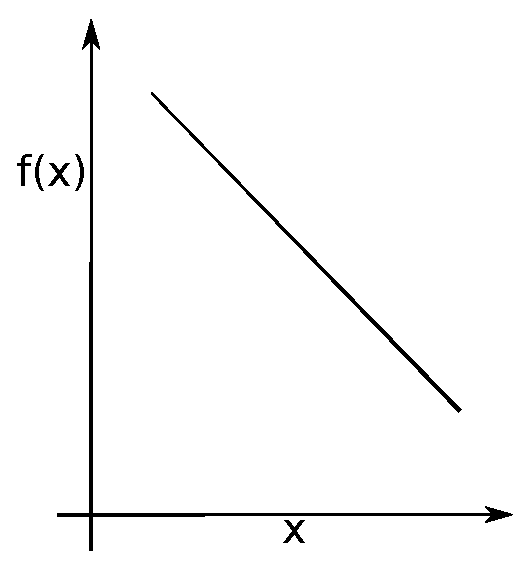
\includegraphics[width=\linewidth]{{{thermodynamics/decreasing}}}
			\caption{negative slope}
		\end{subfigure}
		\begin{subfigure}{0.329\textwidth}
			\centering
			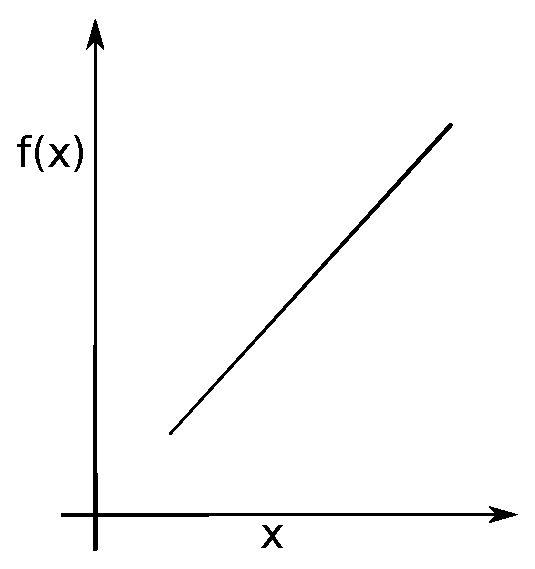
\includegraphics[width=\linewidth]{{{thermodynamics/increasing}}}
			\caption{positive slope}
		\end{subfigure}
		\caption{shape of $f(x)$ from $f^{\prime}(x)$}
		\label{fig:diff1_of_f}
	\end{figure}
	
	If the second derivative of this function is negative (positive) the function is said to have concave (convex) shape (\ref{fig:diff2_of_f}).
	\begin{figure}
		\centering
		\captionsetup[subfigure]{width=0.9\textwidth}
		\begin{subfigure}{0.329\textwidth}
			\centering
			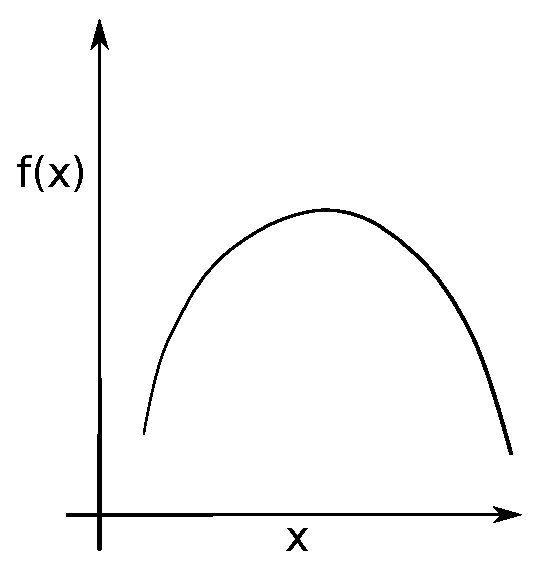
\includegraphics[width=\linewidth]{{{thermodynamics/concave}}}
			\caption{concave}
		\end{subfigure}
		\begin{subfigure}{0.329\textwidth}
			\centering
			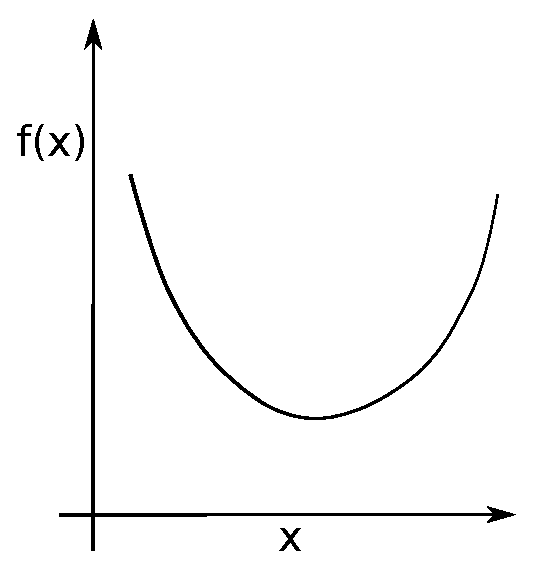
\includegraphics[width=\linewidth]{{{thermodynamics/convex}}}
			\caption{convex}
		\end{subfigure}
		\caption{shape of $f(x)$ from $f^{\prime\prime}(x)$}
		\label{fig:diff2_of_f}
	\end{figure}
	Thus if we know the sign of the first and second derivative we can approximate a shape of the function.
	
	
	\subsection{Free Energy}
	Now since we obtain from (\ref{eqn:gibbs_def}) that the entropy is the first derivative of the free energy (\ref{eqn:entropy_by_gibbs}) and from (\ref{eqn:def2_specific_heat}) specific heat is the second derivative of the free energy (\ref{eqn:specific_heat_by_gibbs}). Since the entropy is a positive quantity and specific heat is also a positive quantity we get that the first and second derivative of the free energy is negative which implies from the laws of calculus that the shape of the free energy should be a decreasing concave curve (\ref{fig:free_energy}) in other words concave shaped with negative slope.
	\begin{equation}
	S = - \frac{\partial G}{\partial T}
	\label{eqn:entropy_by_gibbs}
	\end{equation}
	\begin{equation}
	C = - \frac{\partial^2 G}{\partial T ^2}
	\label{eqn:specific_heat_by_gibbs}
	\end{equation}
	\begin{figure}
		\centering
		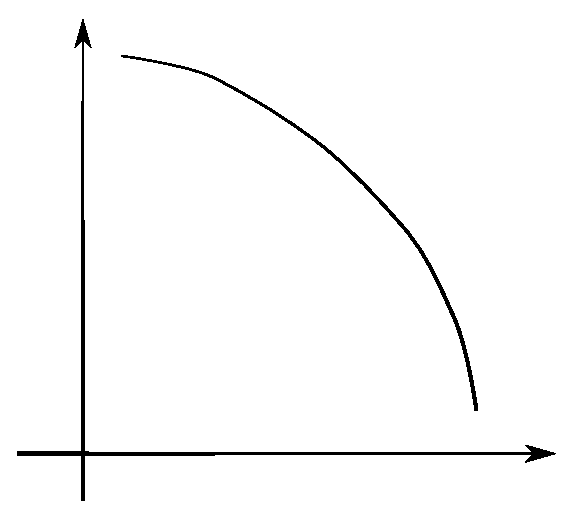
\includegraphics[width=0.3\columnwidth]{{{thermodynamics/free_energy}}}
		\caption{Shape of the free energy}
		\label{fig:free_energy}
	\end{figure}

	\subsection{Entropy and Specific Heat}	
	Now that we know the shapes of the free energy, the very next thing to do is to find the shape of the entropy. Since we can get entropy from differentiating the free energy with respect to temperature $T$ we get the following shape (\ref{fig:entropy_1_2}). From the definition of the transition order we know that the first order transition is discontinuous and the second order transition continuous. Since the first order transition requires latent heat at the critical point the discontinuity is inevitable. Note that, since entropy measures disorderedness of a system it should increase with increasing temperature. Because the temperature is nothing but the average kinetic energy of the particles in the system. As the kinetic energy of the system increases with temperature, the particles tend to vibrate more and get higher average velocity. Thus making the system disordered. Therefore in a physical system entropy always increases with the increasing of temperature. If we find something different, as if, the entropy is decreasing with the increasing of temperature, there must be a problem somewhere.
	\begin{figure}
		\centering
		\captionsetup[subfigure]{width=0.9\textwidth}
		\begin{subfigure}[t]{0.329\textwidth}
			\centering
			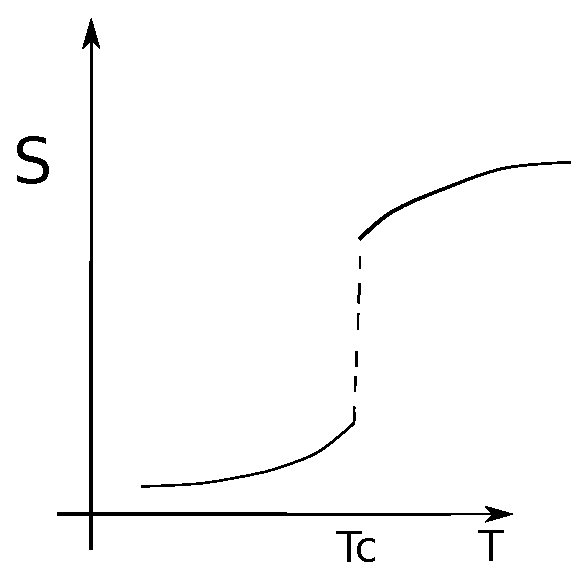
\includegraphics[width=\linewidth]{{{thermodynamics/entropy_1st}}}
			\caption{Entropy in first order transition}
		\end{subfigure}
		\begin{subfigure}[t]{0.329\textwidth}
			\centering
			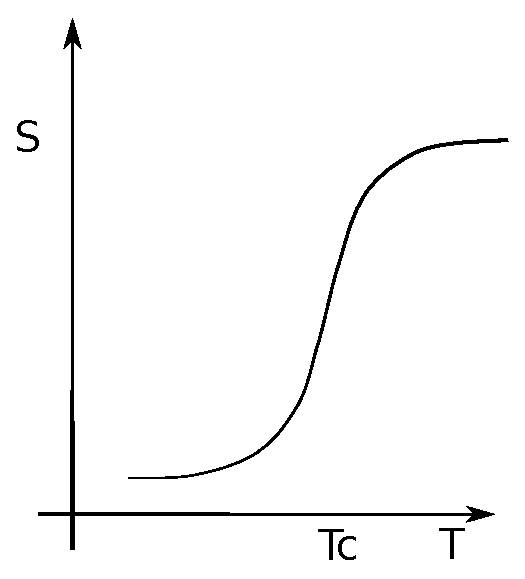
\includegraphics[width=\linewidth]{{{thermodynamics/entropy_2nd}}}
			\caption{Entropy in 2nd order transition}
		\end{subfigure}
		\caption{Shape of entropy}
		\label{fig:entropy_1_2}
	\end{figure}
	Just after knowing the shape of entropy one can anticipate the shape of specific heat, which is the derivative of the entropy with respect to temperature and is defined in (\ref{def:specific-heat-thermodynamics}). Using this and the shape of entropy we can get the shape of the specific heat immediately as in figure (\ref{fig:specific_heat-susceptibility})
	\begin{figure}
		\centering
		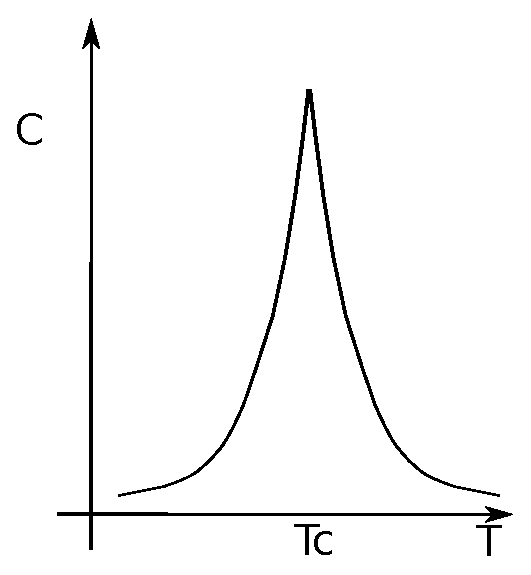
\includegraphics[width=8cm, height=8cm]{{{thermodynamics/specific_heat}}}
		\caption{Shape of Specific Heat and Susceptibility}
		\label{fig:specific_heat-susceptibility}
	\end{figure}
	\subsection{Order Parameter and Susceptibility}
	Since diamagnetic substances have negative susceptibilities $(\chi < 0)$; paramagnetic, and ferromagnetic substances have positive susceptibilities $(\chi > 0)$, and we are working for a phase transition model similar to paramagnet and ferromagnet transition, taking susceptibility to be positive is appropriate for our model. Now if susceptibility is positive then from (\ref{eqn:susceptibility_def}) we get $\left(\frac{\partial^2G}{\partial h ^2}\right) < 0$ which means that the shape of the free energy for this case is concave from the knowledge of (\ref{sec:determine_shape_using_calculus}). And from (\ref{eqn:magnetization_def}) and the fact that the magnetic field $h$ can be positive or negative, as it can change direction, the Gibbs free energy is negative, since it is the lowest binding energy. \\
	Also from (\ref{eqn:susceptibility_def2}) we can say $\frac{\partial^2 A}{\partial m ^2}$ is positive giving convex shape of the Helmholtz free energy. And (\ref{eqn:mag_field_def}) tells us that since $h$ can ve positive or negative, the Helmholtz free energy can have increasing or decreasing slope respectively.
	


%------------------------------------------------------------------------------------
\section{Critical Exponents}
	Near the critical point there is, in general, a function that describes the behavior of the system that is mostly interesting. For thermodynamical system the temperature is the control parameter , thus that function depends on the temperature. But since we want the information at the critical point, $(T-T_c)/T_c$, instead of $T$ is a better parameter to address. In equation
	\begin{equation}
		\epsilon = \frac{T-T_c}{T_c} = \frac{T}{T_c} - 1
	\end{equation}
	$\epsilon$ is considered a better parameter. Thus a function $f(\epsilon)$ is used instead of $f(T)$. Using the fact that in the vicinity of $T_c$ the function $f(\epsilon)$ exhibits power law
	\begin{equation}
		f(\epsilon) \sim \epsilon^\lambda
	\end{equation}
	The following figures shows some function that exhibit power law
	\begin{figure}
		\centering
		\captionsetup[subfigure]{width=0.9\textwidth}
		\begin{subfigure}[t]{0.4\textwidth}
			\centering
			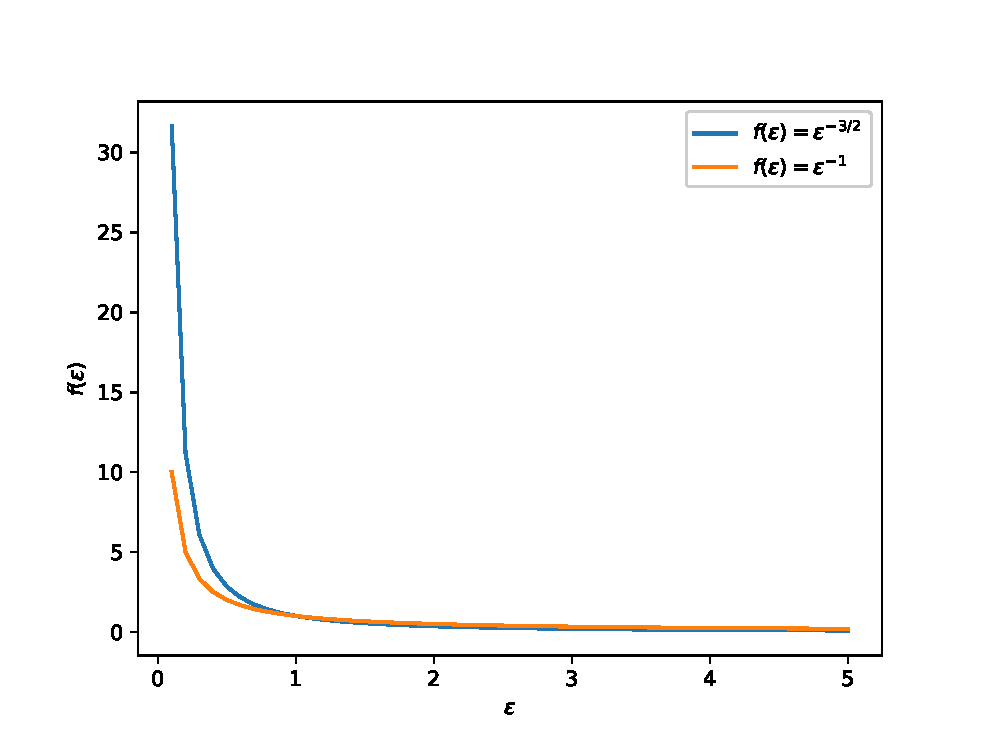
\includegraphics[width=\linewidth]{{{power_law_functions/fig1}}}
			\caption{$f(\epsilon) \sim \epsilon^\lambda$ where $\lambda=-1,-3/2$}
		\end{subfigure}
		\begin{subfigure}[t]{0.4\textwidth}
			\centering
			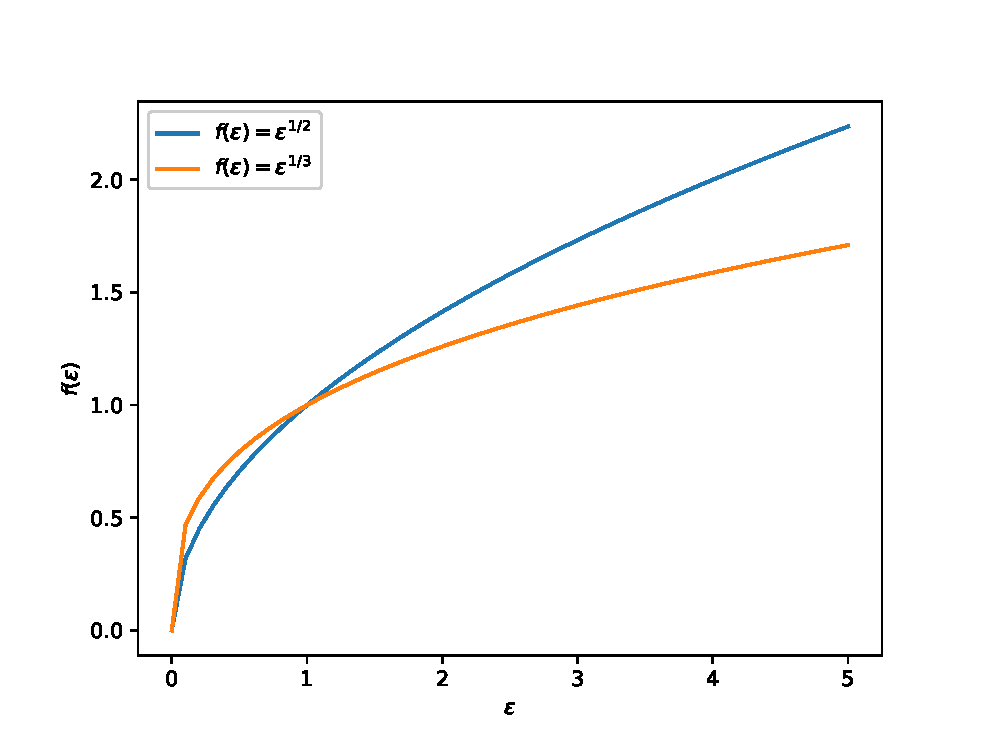
\includegraphics[width=\linewidth]{{{power_law_functions/fig2}}}
			\caption{$f(\epsilon) \sim \epsilon^\lambda$ where $\lambda=1/2,1/3$}
		\end{subfigure}
		\caption{Function showing power law}
	\end{figure}
	To see this more closely, we can expand any function $f(\epsilon)$ as a power series of $\epsilon$
	\begin{equation}
		f(\epsilon) = A \epsilon^\lambda ( 1 + B \epsilon^a + C \epsilon^b + ...)
	\end{equation}
	Near $T_c$ only the first term is dominating.
	We had the Gibbs free energy (for a magnetic system)
	\begin{equation}
		G = G(T,h) \equiv G(\epsilon, h)
	\end{equation}
	since $\epsilon$ is a better parameter. Assuming that $G$ is a generalized Homogeneous function. Therefore from the realization of section (\ref{sect:homogenious-function}) we can write
	\begin{equation}
		G(\lambda^{a_\epsilon} \epsilon, \lambda^{a_h} h) = \lambda G(\epsilon, h)
		\label{eqn:gibbs_homogenious}
	\end{equation}
	differentiating equation (\ref{eqn:gibbs_homogenious}) with respect to $h$
	\begin{align}
		\frac{\partial G(\lambda^{a_\epsilon} \epsilon, \lambda^{a_h} h)}{\partial h} &= \lambda \frac{\partial G(\epsilon, h)}{\partial h} \nonumber \\
		\frac{\partial G(\lambda^{a_\epsilon} \epsilon, \lambda^{a_h} h)}{\partial \lambda^{a_h} h} \lambda^{a_h} &= \lambda \frac{\partial G(\epsilon, h)}{\partial h} \nonumber \\
		\lambda^{a_h} G^\prime(\lambda^{a_\epsilon} \epsilon, \lambda^{a_h} h) &= \lambda G^\prime (\epsilon, h) \nonumber \\
		-\lambda^{a_h} m(\lambda^{a_\epsilon} \epsilon, \lambda^{a_h} h) &= -\lambda m(\epsilon, h) \nonumber \\
		m(\lambda^{a_\epsilon} \epsilon, \lambda^{a_h} h) &= \lambda^{1-a_h} m(\epsilon, h) \\
		\label{eqn:order_parameter_homogeneous}
	\end{align}
	Here $m$ is the magnetization or order parameter. The figure (\ref{fig:shape-order-parameter}) shows the general shape of the order parameter.
	\begin{figure}
		\centering
		\includegraphics[width=10cm, height=10cm]{{{order-parameter}}}
		\caption{General shape of Order Parameter}
		\label{fig:shape-order-parameter}
	\end{figure}

	Setting $h=0$ in equation (\ref{eqn:order_parameter_homogeneous})
	\begin{align}
		m(\lambda^{a_\epsilon} \epsilon)	 &= \lambda^{1-a_h} m(\epsilon) \nonumber \\
		m(1)	 &= \lambda^{1-a_h} m(\epsilon) \nonumber \\
		m(1)	 &= \epsilon^{-\frac{1-a_h}{a_\epsilon}} m(\epsilon) \nonumber \\
		m(\epsilon) &= \epsilon^\beta m(1) \label{eqn:order_parameter_and_beta}
	\end{align}
	where
	\begin{equation}
		\beta = \frac{1-a_h}{a_\epsilon}
		\label{eqn:beta}
	\end{equation}
	Note that, setting $\lambda^{a_\epsilon} \epsilon = 1$ gives $\lambda = \epsilon^{-1/a_\epsilon}$.\\
	Setting $\epsilon=0$ in equation (\ref{eqn:order_parameter_homogeneous})
	\begin{align}
		m(\lambda^{a_h} h) &= \lambda^{1-a_h} m(h) \nonumber \\
		m(1) &= h^{-\frac{1-a_h}{a_h}} m(h) \nonumber \\
		m(h) &= m(1) h^\delta \label{eqn:order_parameter_and_delta}
	\end{align}
	where
	\begin{equation}
		\delta = \frac{a_h}{1-a_h}
		\label{eqn:delta}
	\end{equation}
	Again, note that, setting $\lambda^{a_h} h = 1$ gives $\lambda = h^{-1/a_h}$\\
	Now, Since the response functions are the second derivative of the free energy (\ref{sect:response-functions}), by differentiating (\ref{eqn:gibbs_homogenious}) twice with respect to $\epsilon$ we get the Specific Heat
	\begin{align}
		\lambda^{2 a_\epsilon} G^{\prime\prime}(\lambda^{a_\epsilon} \epsilon, \lambda^{a_h} h) &= \lambda G^{\prime \prime}(\epsilon, h) \nonumber \\
		\lambda^{2 a_\epsilon} \frac{\partial G(\lambda^{a_\epsilon} \epsilon, \lambda^{a_h} h)}{\left(\frac{1}{T_c}\right)^2 \partial T^2} &= \lambda G^{\prime \prime}(\epsilon, h) \nonumber \\
		\lambda^{2 a_\epsilon} C(\lambda^{a_\epsilon} \epsilon, \lambda^{a_h} h) &= \lambda C(\epsilon, h)
		\label{eqn:specific_heat_homogeneous}
	\end{align}
	We have used $\epsilon = \frac{T}{T_c} -1$ and $d\epsilon = \frac{1}{T_c} dT$. Now setting $h=0$ we get from (\ref{eqn:specific_heat_homogeneous})
	\begin{align}
		\lambda^{2 a_\epsilon} C(\lambda^{a_\epsilon} \epsilon) &= \lambda C(\epsilon) \nonumber \\
		C(1) &= \lambda^{1- 2 a_\epsilon} C(\epsilon) \nonumber \\
			 &= \epsilon^{-\frac{1-2 a_\epsilon}{a_\epsilon}} C(\epsilon) \nonumber \\
		C(\epsilon) &= \epsilon^{-\alpha} C(1) \label{eqn:specific_heat_and_alpha}
	\end{align}
	We have used the value of $\lambda$ when we set $\epsilon \lambda^{a_\epsilon}=1$ and the exponent
	\begin{equation}
		\alpha = \frac{2 a_\epsilon - 1}{a_\epsilon}
		\label{eqn:alpha}
	\end{equation}
	
	Again by differentiating (\ref{eqn:gibbs_homogenious}) twice with respect to $h$ we get the susceptibility. Then we set $h=0$ to get only $\epsilon$ dependency.
	\begin{align}
		\lambda \frac{\partial^2 G(\epsilon,h)}{\partial h^2} &= \lambda^{2 a_h} \frac{\partial^2 G(\lambda^{a_\epsilon} \epsilon, \lambda^{a_h} h)}{\partial h^2} \nonumber \\
		\lambda \chi(\epsilon, h) &= \lambda^{2 a_h} \chi(\lambda^{a_\epsilon}\epsilon, \lambda^{a_h} h) \nonumber \\
		\chi(\epsilon) &= \lambda^{2 a_h - 1} \chi(\lambda ^{a_\epsilon} \epsilon) \nonumber \\
		\chi(\epsilon) &= \epsilon^{-\gamma} \chi(1) 
		\label{eqn:susceptibility_homogeneous}
	\end{align}
	Similar to previous case, We have used the value of $\lambda$ when we set $\epsilon \lambda^{a_\epsilon}=1$ and the exponent is
	\begin{equation}
		\gamma = \frac{2 a_h -1}{a_\epsilon}
		\label{eqn:gamma}
	\end{equation}
	\subsection{List of Thermodynamic Quantities that Follows Power Law}
	\label{subsect:list-of-exponents}
	
		The exponent that scales Specific heat is called $\alpha$ 
		\begin{equation}
			C \sim \epsilon^{-\alpha}
		\end{equation}
		The exponent that scales order-parameter is called $\beta$ 
		\begin{equation}
			m \sim \epsilon^{\beta}
		\end{equation}
		Another exponent that scales order-parameter is called $\delta$, but it relates the order parameter with the magnetic field, $h$
		\begin{equation}
			m \sim h^{\delta}
		\end{equation}
		The exponent that scales susceptibility is called $\gamma$ 
		\begin{equation}
			\chi \sim \epsilon^{-\gamma}
		\end{equation}
		Note that these quantities only follows power law near $T_c$.
	\subsection{Rushbrooke Inequality}
		\begin{equation}
			\alpha + 2 \beta + \gamma \ge 2
		\end{equation}
		but the equality is often obtain theoretically which is shown below in the present case 
		\begin{align}
			\alpha + 2\beta + \gamma &= \frac{2 a_\epsilon -1}{a_\epsilon} 
					+ \frac{2 (1 - a_h)}{a_\epsilon}
					+ \frac{2 a_h - 1}{a_\epsilon} \nonumber \\
					&= \frac{2 a\epsilon}{a\epsilon} \nonumber \\
					&= 2 \nonumber
		\end{align}
	Thus the Rushbrooke inequality is satisfied.
	\subsection{Griffiths Inequality}
	\begin{equation}
		\alpha + \beta (1+\delta)  = 2
	\end{equation}
	Let's do a quick check to see if this is also satisfied.
	\begin{align}
		\alpha + \beta (1+\delta) &= \frac{2 a_\epsilon - 1}{a_\epsilon} 
									+ \frac{1 - a_h}{a_\epsilon} \left(1 + \frac{a_h}{1 - a_h}\right) \nonumber \\
								  &= \frac{2 a_\epsilon - 1}{a_\epsilon}  + \frac{1}{a_\epsilon} \nonumber \\
								  &= \frac{2 a_\epsilon}{a_\epsilon} \nonumber \\
								  &= 2 \nonumber \\
	\end{align}
	So the Griffiths Inequality is also satisfied. 
	
	
	
\section{Ising Model}
	For a very long time scientists have been trying to understand phase transition in different aspects. And for this purpose many different models have been provided for decades. The first model was provided by physicist Ernst Ising as a mathematical model of ferromagnetism in statistical mechanics. 
	The Ising model was invented by the physicist Wilhelm Lenz (1920), who gave it as a problem to his student Ernst Ising. The one-dimensional Ising model has no phase transition and was solved by Ising (1925) himself in his 1924 thesis \cite{Ising1925}.
	But he provided a model in 1 dimension and proved that in 1 dimension phase transition is not possible and concluded that it is not possible in higher dimension as well. But it was proved later that in dimension $d \geq 2$ phase transition is possible \cite{Yang1952, Montroll1963} which proved Ising wrong about his conclusion but he certainly gave a good insight for phase transition and hence the naming.
	
	Consider a set $\Lambda$ of lattice sites, each with a set of adjacent sites forming a d-dimensional lattice. For each lattice site $k\in\Lambda$ there is a discrete variable $\sigma_k$ such that $\sigma_k \in \{+1, -1\}$, representing the site's spin. A spin configuration $\sigma = \left(\sigma_k\right)_{k\in\Lambda}$ is an assignment of spin value to each lattice site.
	
	For any two adjacent sites $i,j \in \Lambda$ there is an interaction $J_{ij}$. Also a site $j\in \Lambda$ has an external magnetic field $h_j$ interacting with it. The energy of a configuration $\sigma$ is given by the Hamiltonian
	\begin{equation}
		H(\sigma) = - \sum_{<i j>} J_{ij} \sigma_i \sigma_j - \mu \sum_{j} h_j \sigma_j
	\end{equation}
	Where the first sum is over pairs of adjacent spins counting every pair only once. And we use $<ij>$ to indicate that $i$ and $j$ are nearest neighbors. $\mu$ indicates the magnetic moment. The negative sign on the second term is there by convention \cite{Baierlein1999}. The configuration probability is given by the Boltzmann distribution with inverse temperature $\beta \geq 0$
	\begin{equation}
		P_\beta (\sigma) = \frac{e^{- \beta H(\sigma)}}{Z_\beta}
	\end{equation}
	where $\beta = \left(k_B T\right)^{-1}$ and the normalization constant
	\begin{equation}
		Z_\beta = \sum_\sigma e^{-\beta H(\sigma)}
	\end{equation}
	is the partition function. For a function $f$ of the spins, which is the observable here, we denote
	\begin{equation}
		<f>_{\beta} = \sum_{\sigma} f(\sigma) P_\beta(\sigma)
	\end{equation}
	the expectation value of $f$.
	The configuration probabilities $P_\beta(\sigma)$ represent the probability that the system in in a state with configuration $\sigma$ in equilibrium.
	
	
	The minus sign on each term of the Hamiltonian function $H(\sigma)$ is conventional. Using this sign convention, the Ising models can be classified according to the sign of the interaction: if, for all pairs $i,j$
	\begin{equation}
	J_{ij}
	\begin{cases}
		 > 0 \text{, ferromagnetic interaction }\\
		 < 0 \text{, anti-ferromagnetic interaction}\\
		 = 0 \text{, non-interacting spins}
	\end{cases}
	\end{equation}
	
	otherwise the system is called non-ferromagnetic.
	
	In a ferromagnetic Ising model, spins tend to be aligned, meaning, the configurations in which adjacent spins are of the same sign have higher probability. In an anti-ferromagnetic model, adjacent spins tend to have opposite signs.
	
	The sign convention of $H(\sigma)$ also explains how a spin site $j$ interacts with the external field. Namely, the spin site wants to line up with the external field.
	
	\begin{equation}
	h_j
	\begin{cases}
		 > 0 \text{,  the spin site $j$ desires to line up in the positive direction} \\
		 > 0 \text{,  the spin site $j$ desires to line up in the negative direction} \\
		 = 0 \text{,  no external influence on the spin site}
	\end{cases}
	\end{equation}



	Ising models are often examined without an external field interacting with the lattice, that is, $h = 0$ for all $j$ in the lattice $\Lambda$. Using this simplification, our Hamiltonian becomes:
	\begin{equation}
		H(\sigma) = - \sum_{<i j>} J_{i j} \sigma_i \sigma_j
	\end{equation}
	When the external field is everywhere zero, $h = 0$, the Ising model is symmetric under switching the value of the spin in all the lattice sites; a non zero field breaks this symmetry.
	
	Another common simplification is to assume that all of the nearest neighbors $<ij>$ have the same interaction strength. Then we can set $J_{ij} = J$ for all pairs $i,j$. In this case our Hamiltonian is further simplified to:
	
	\begin{equation}
		H(\sigma) = - J \sum_{<i j>} \sigma_i \sigma_j
	\end{equation}
	
	Ising himself had provided the theory of his model for $1$ dimensional case. He did not find any phase transition and concluded that phase transition is not possible in any dimension. 
	
	Consider an one dimensional lattice where all sites are in spin up state. Then according to Ising model their total energy $E$ and entropy $S$ is as follows
	\begin{align}
		E &= -N J \\
		S &= 0
	\end{align}
	Where $N$ is the number of sites on the lattice. Now if one of the sites is fliped then
	\begin{align}
		E &= - (N-2)J \\
		S &= \log N
	\end{align}
	Therefore the cost is $\Delta E = 2J$ and change in entropy is $\Delta S = \log N$ for flipping spin of one site. The figure (\ref{fig:1d-ising-model}) shows this.
	\begin{figure}
		\centering
		\begin{subfigure}[t]{0.4\textwidth}
			\centering
			\includegraphics[height=0.6cm]{{{ising-1d-0}}}
			\caption{all are in spin up state}
		\end{subfigure}
		\begin{subfigure}[t]{0.4\textwidth}
			\centering
			\includegraphics[height=0.6cm]{{{ising-1d-1}}}
			\caption{only one site is in spin down state}
		\end{subfigure}
		\caption{One dimensional Ising model}
		\label{fig:1d-ising-model}
	\end{figure}
	
	Therefore the change in free energy due to flipping one spin is,
	\begin{align}
		\Delta F &= \Delta E - T \Delta S \\
				 &= 2J - T \log N
	\end{align}
	In the thermodynamic limit $N \rightarrow \infty$ the second term always dominates except for $T=0$. Thus in one dimensional lattice there is phase transition at non zero temperature sice we cannot have $\Delta F=0$ (the transition point).
	
	
	Now interesting this happens in case of two dimensional lattice. Say we have a square lattice of size $N$ where there is an island of $L=3$ sites of different spins (\ref{fig:2d-ising-model}).
	\begin{figure}
		\centering
		\includegraphics[width=5cm]{{{ising-model-2d}}}
		\caption{Two dimensional Ising model with an island of 3 site with opposite spin state}
		\label{fig:2d-ising-model}
	\end{figure}
	\begin{align}
		\Delta E &= 2 L J \\
		\Omega &= 3^L N \\
		S &= K \log \Omega \\
		\Delta S &= S - 0 = S
	\end{align}
	Therefore the free energy is 
	\begin{align}
		\Delta F 
		&= \Delta E - T\Delta S \\
		&= 2JL - KT\log (3^L N) \\
		&= 2 J L - T L \log 3 - K T \log N
	\end{align}
	since at transition point $\Delta F = 0$ we get
	\begin{align}
		0 &= L(2J - T_c \log 3) \\
		T_c &= \frac{2J}{\log 3}
	\end{align}
	clearly $J\neq 0$ then $T_c \neq 0$.
	The exact solution is 
	\begin{equation}
		T_c = \frac{2J}{\log(1 + \sqrt{2})}
	\end{equation}
	Thus we can see that spontaneous magnetizaion (phase transition) is possible in 2D for a non zero $T$. And any higher dimensional lattice undergoes a transition for a non zero temperature.
	
	

%!TEX root = ../thesis.tex
%*******************************************************************************
%****************************** Fourth Chapter **********************************
%*******************************************************************************
\chapter{Percolation Theory}

% **************************** Define Graphics Path **************************
\ifpdf
    \graphicspath{{Chapter4/Figs/}{Chapter4/Figs/playground/}{Chapter4/Figs/entropy_cluster/}}
\else
    \graphicspath{{Chapter4/Figs/}{Chapter4/Figs/playground/}{Chapter4/Figs/entropy_cluster/}}
\fi

Percolation theory potentially has been of great interest as it can describe many phenomena \cite{Sahini1994}. New models and variants of existing model is always welcome due to its importance and of wide interdisciplinary interests. In recent decades there has been a surge of research activities in studying percolation thanks to the emergence of network which has been used as the skeleton for percolation which can mimic structure of many natural and man-made systems.\\

There are several reason to study percolation. First, it is easy to formulate and simple to implement as there is only one control parameter, called occupation probability $p$ \ref{subsect:occupation-probability}. Second, scientists use it as a theoretical model for phase transition, just like architects use geometric model before building large expensive structure, because of its simplicity. Third, it is well endowed with beautiful features and conjectures like finite-size scaling, universality just like its thermal counterpart. Fourth, besides being the paradigmatic model for phase transition, it has been found that the notion of percolation is omnipresent in a wide range of many seemingly disperate systems \ref{sect:application}.\\

To study percolation theoretically, the first thing that one need is to choose a skeleton or playground, namely an empty lattice (or a graph/network), consisting of sites (or nodes) and bonds (or links). The definition of the percolation model is then so simple that it merely needs a sentence to define it. Each site or bond of the chosen skeleton, depending on whether we want to study site or bond type percolation, is either occupied with probability p or remains empty with probability $1-p$ independent of the state of its neighbors. Recently, percolation has received a renewed attention due to widening scope for using complex networks as a skeleton and due to widening extent of using various variants as a rule. In percolation most observable quantities this way or another is connected to clusters, group of contiguous occupied sites form a cluster, or to their distribution function. As the occupation probability p is tuned starting from $p = 0$, one finds that at certain value of $p=p_c$ the observable quantities undergoes a sudden and sharp change which is always regarded as a sign of phase transition. Indeed, the value at which such change occurs is called threshold or critical value which is equivalent to critical temperature of its thermal counterpart. The phase transition that percolation describes
is purely geometrical in nature. It requires no consideration of quantum and many particle interaction effects and hence we can use it as a model for thermal Continuous Phase Transition (CPT) like artichect use model before constructing large and complicated structure

\section{Percolation Phenomena}
	The word 'Percolation' comes from the coffee percolator but it has nothing to do with	coffee brewing. The only connection might be in the concept that lies behind the name.	Let's start explaining the phenomena by example. Let's consider a square grid made of conductor of	size $L\times L$ containing $L^2$ sites (insulator).% and $2 L^2$ bonds.
    Now we set up an arrangement to put a potential difference across the square grid and measure the effective resistance of the grid as well	as the current. Suppose now we start taking of the sites one by one at a random and place a conductor there. We	define a parameter called Occupation Probability, $p$, which is the fraction of the  sites replaced as conductor to the total number of sites. We visit all the sites and generate a random number and only if $r <= p$ we replace the site with a conductor. We observe that the electric	conductance of the grid will be found to increase with increasing sites being replaced by conductors. As the sites are being turned into insulators, the value of $p$ changes. We see that at a	certain value of $p$ , the electricity starting flowing. This particular value is known as Percolation Threshold, $p_c$ . This vanishing resistance occurs when a particular amount of sites turns into conductors from insulators that causes the system to get the connection	between the two end across polarity. The exact value of $p_c$ has been found to be close to $0.5927$. One can never expect to get the	value each time they perform this experiment, infact, the chance of getting this exact	value at any experiment can be one in a million. So we do this same experiment a	number of times and then average over the value to get a better result. This example shows a simple way of understanding the phenomenon that we call
	percolation. The theory which simulates this kind of phenomenon is known as Percolation Theory. It provides a quantitative description of the nature of continuous pathways through space. The usual objective of research implementing this phenomenon	is to characterize some aspect of the critical phenomena of the phase transition between finite and infinite range connectivity. This is actually non-trivial when the space	is randomly disordered and the connected regions acquire fractal properties \cite{Zimm1949, Mandelbrot1983}.
	\begin{figure}
		\centering
		\captionsetup[subfigure]{width=0.9\textwidth}
		\begin{subfigure}[t]{.45\textwidth}
			\centering
			\includegraphics[width=0.8\linewidth]{{{square-lattice-spanning-cluster-0}}}
			\caption{One step away to flow current from top to bottom only if the gray site is next to be occupied.}
		\end{subfigure}
		\begin{subfigure}[t]{.45\textwidth}
			\centering
			\includegraphics[width=0.8\linewidth]{{{square-lattice-spanning-cluster-1}}}
			\caption{Current flows from top to bottom for the first time, i.e. $p=p_c$.}
		\end{subfigure}
		\caption{percolation phenomena in square structure. No current if $p<p_c$.}
	\end{figure}

\section{Historical Overview}
	In 1941, the idea of percolation was first conceived by Flory \cite{Flory1941} in the context of gelation transition. But as a mathematical model, it was formulated in the late fifties, to understand the motion of gas molecules through the maze of pores in carbon granules filling a gas mask. This seminal work was done by Simon Broadbent and John Hammersley \cite{Broadbent1957}, an engineer and a mathematician respectively. Later on, percolation problem was popularized in physics community by Cyril Domb, Michael Fisher, John Essam and M.F. Skyes \cite{Essam1980, Fisher1961}. Another remarkable work was the observation of percolation to be the limiting case of the general Potts model, which includes the Ising model and can be solved exactly which is done by Fortuin and Kasteleyn in 1969 \cite{Kasteleyn1969}. This work paved the way to many exact results in percolation, and also 	allowed the usage of powerful re-normalization group ideas \cite{Cardy1996}. Finding percolation threshold both exactly and by simulation has been an enduring subject of research in	this field \cite{Schrenk2013}, as well as the development of algorithms such as those by Hoshen and	Kopelman \cite{Hoshen1976}, by Leath \cite{Leath1976}, and by Newman and Ziff \cite{Newman2001} (which we have used in	our research). Finding rigorous proofs of exact thresholds and bounds has also been an enduring area of research for mathematicians (Kesten \cite{Kesten1987}, Wierman \cite{Wierman1984}, Bollobas	and Riordan \cite{Bollobs2010} etc.) Another infusion of interest in percolation came from the surgin	field of network theory which goes back to the study of random and complete graphs	by Erdos-Renyi(1959). In ER model, an observation of made of formation of a giant	component, this giant component is exactly analogous to the formation pattern in percolation \cite{Erdos1959, Erdos1964}. It was then revitalized by interest in the small world phenomenon and	Scale free networks. In 2000, Newman and Moore found the critical point for a random	graph in the limit of large size, in which case the system is effectively a Bethe lattice,	and this result connects to the early work of Flory, Fisher and Essam, but it was found
	with a general degree distribution \cite{Moore2000}. In the field of random networks, the model of	explosive percolation was first introduced by Achlioptas, D'Souza and Spencer \cite{Achlioptas2009},	and this has been another fascinating problem which has led to a wave of new interest	in percolation.

\section{Classifications and Playground}
	Any percolation problem have two major parts, one is the rule which states how and what to occupy and connect and another is a playground on which we apply the rules. The term spanning cluster is the cluster that connects the opposite boundary of a playground. If, however, the system has no boundary then it is measured in terms of largest cluster and is called Giant Connected Component or GCC and it only appears if the system has reached or passed the threshold. 
		
	\subsection{Types of Percolation}
		Since the first percolation model studied was Bernoulli percolation (In this model all bonds are independent. This model is called bond percolation by physicists) through time physicists have defined different types of percolation model in different types of skeleton or playground. Here we discuss some of the most used percolation types.
		
		\subsubsection{Bond Percolation}
			In bond (or edge, link) percolation we occupy the bonds with probability $p$ and we use sites to connect the bonds together. The cluster size is measured in terms of the number of sites in the cluster. If $p$ is below a critical value $p_c$ then there is no spanning cluster (or GCC) and if $p \geq p_c$ then we will have a spanning cluster or GCC.
			
			
		\subsubsection{Site Percolation}
			In site (or vertex, node) percolation we occupy the sites. According to the definition of site percolation we use sites to measure the cluster size. But in order to keep it consistent with the laws of thermodynamics we have changed the definition \cite{redefinition-of-site-percolation}. Now we use bonds to measure the cluster size while we occupy sites. This change of definition does not effect the exponent that describe the phase transition. Before the critical point where $p<p_c$ there is not spanning cluster and if $p=p_c$ the spanning cluster appears for the first time and it remains as the largest cluster of the system. All the property that describes the phase transition are present at $p=p_c$ and this is where we study them.


		\subsubsection{Explosive Percolation}
		% citation completed
		In 2009 Achlioptas et al. proposed a biased occupation rule, known as the Achlioptas process (AP), that encourages slower growth of the larger clusters and faster growth of the smaller clusters	instead of random occupation in classical percolation \cite{Achlioptas2009}. According to this rule a pair of links	or, bonds are first picked uniformly at random from all possible distinct links. However, of the		two, only the one that satisfies the pre-selected rule is finally chosen to occupy and the other one	is discarded. The preset rule is usually chosen so that it discourages the growth of the larger	clusters and encourages the growth of the smaller clusters. As a result, the percolation threshold is delayed and hence the corresponding $p_c$ is always higher than the case where only one bond is	always selected. Furthermore, it is natural to expect that close to $p_c$ nearly equal sized clusters, waiting to merge, are so great in number that occupation of a few bonds results in an abrupt global	connection and thus the name "Explosive Percolation" (EP). Investigation of Achlioptas processes on different types of substrate networks and with different choices of rules especially with the aim	of developing rules that do not use global information about a graph is an active area of research.


		\subsubsection{K-Core Percolation}
		% citation completed
		The $K$-core of an unweighted, undirected network is the maximal subset of nodes such that each node is connected to at least $K$ other nodes \cite{Seidman1983}. Determining $K$-cores computationally is fast and they are insightful in many situations \cite{Dorogovtsev2006,Csermely2013}. Every undirected, unweighted network has a $K$-core decomposition. $K$-shell of a network is defined as the set of all nodes that belong to the $K$-core but not to the $(K+1) $- core. $K$-core is given by the union of all $c$-shells for $c>=K$ and the $K$-core decomposition is the set of all of its $c$-shells. One can examine the $K$-core of a network as the limit of a dynamical pruning process. Starting with the initial network we delete all nodes with fewer than $k$ neighbors. After this pruning, the degree of some of the remaining nodes will have been reduced. Repeating this process to delete nodes will give a network which will have fewer than $K$ remaining neighbors. Iterating this process until no further pruning is possible leaves the $K$-core of the network \cite{Porter2016}.


		\subsubsection{Bootstrap Percolation}
		% citation completed
		Bootstrap percolation is an infection-like process in which nodes becomes infected if sufficiently many of their neighbors are infected \cite{Adler1991}. In bootstrap percolation, sites on an empty lattice are first randomly occupied and then all occupied sits with less than a given number $m$ of the occupied neighbors are successively removed until a stable configuration reached. On any lattice for sufficiently large $m$, the ensuing clusters can  only be infinite. On a Bethe lattice for $m\geq 3$, the fraction of the lattice occupied by infinite clusters discontinuously jumps from zero at the percolation threshold. From an analysis of stable and metastable ground state of the dilute Blume-Capel model \cite{Blume1966}, it is concluded that the effects like bootstrap percolation may occur in some real magnets \cite{Chalupa1979}.


		\subsubsection{Other}
		% citation completed
		Apart from the type of percolation process described briefly above there are numerous other types of percolation. In \textit{Limited Path Percolation}, one construes "connectivity" as implying that sufficiently short path still exists after some network components have been removed \cite{Lpez2007}. The percolation of $K$-cliques (completely connected sub-graphs of $K$ nodes) has been used to study the algorithmic detection of dense sets of nodes known as "communities" \cite{Palla2005}. Various percolation processes have also been studied in several different types of multi-layer networks (e.g. multiplex networks and interdependent networks) \cite{Boccaletti2014, Kivela2014}. Another class of models results if we remove the restriction of a lattice and allow particles to occupy positions which vary continuously in space. \textit{Continuum Percolation} \cite{Hall1985,Penrose1998,Bogu2009}, as it is called, suffers from the added complication that tricks which can sometimes be used on lattice models cannot be applied. A quite different process as \textit{Invasion Percolation} \cite{Furuberg1996,Mloy1992, Wilkinson1983}; its invention was prompted by attempts to understand flow in porous media. Random numbers are assigned to each site of a lattice. Choose a site, or sites, on one side of the lattice and draw a bond to the neighbor which has the lower random number assigned to it. (The growing cluster represents the invading fluid with the remainder of the sites representing the initial, or defending, fluid). This process continues until the cluster reaches the other side \cite{Lenormand1985}.



		\subsection{Types of Playground}
		Apart from the rules we need a playground to study percolation. Most used playground is described in the following.
		
		
		\subsubsection{Lattice}
		Percolation was mainly studied on different types of lattice. For example, Honeycomb lattice, Bethe lattice, Simple Cubic lattice, Body-Centered-Cubic lattice, Face-Centered-Cubic lattice. In $1998$ Christian D. Lorenz et al. did extensive Monte Carlo simulation to study bond percolation on the simple cubic, face-centered-cubic and body-centered-cubic lattices using epidemic approach. There simulations provide very precise values of the critical thresholds \cite{Lorenz1998}. They calculated Fisher exponent, $\tau$, the finite-size correction exponent, $\Omega$ and the scaling function exponent, $\sigma$ confirmed to be universal. They also did percolation on the HCP (hexagonal closed packed) lattice \cite{Lorenz2000}. Before that in $1981$ JC Wireman studied bond percolation on honeycomb and triangular lattices \cite{Wierman1981}.
		\begin{figure}
			\centering
			\includegraphics[width=\linewidth]{{{cubic}}}
			\caption{Different types of cubic lattice \cite{cubic-lattices}}
			\label{fig:cubic-lattice}
		\end{figure}

		\begin{figure}
			\centering
			\captionsetup[subfigure]{width=0.9\textwidth}
			\begin{subfigure}[t]{.45\textwidth}
				\centering
				\includegraphics[width=\linewidth]{{{triangular}}}
				\caption{Triangular Lattice \cite{cubic-lattices}}
			\end{subfigure}
			\begin{subfigure}[t]{.45\textwidth}
				\centering
				\includegraphics[width=\linewidth]{{{honeycomb}}}
				\caption{Honeycomb Lattice \cite{honeycomb-lattice}}
			\end{subfigure}

			\caption{Different types of cubic lattice}
			\label{fig:honeycomb-triangular-lattice}
		\end{figure}
		Furthermore, an exact solution on Bethe lattice for high density percolation was  done by G. R. Reich and P. L. Leath in 1978 \cite{Reich1978} and J. Chalupa et al. did bootstrap percolation on Bethe lattice in the following year \cite{Chalupa1979}.
		
		
		\subsubsection{Graph or Network}
		A new playground was added to the world of percolation in 1959 when two prominent	mathematicians of all time, Paul Erdos and Alfred Renyi introduced Random Graphs 	\cite{}. Before that, it was mostly popular among the mathematicians but not that		much fascinating for most of the physicists because of its abstraction. But with the advent of scale free networks \cite{Barabasi1999} which mimics the real life networks such as citation		network, social network, protein-protein interaction, in 1999, physicists became much		more interested in random networks. The difference in the terminology like graphs		and networks are just graphs are mostly used by mathematicians and computer scientists and networks is mainly referred by physicists to the same concept. Duncan S.		Callaway and his group did percolation study to find robustness and fragility \cite{Callaway2000}.	Clique percolation is also studied on random networks \cite{Dernyi2005}. A critical phenomenon		analysis on random networks for core percolation is done by Bauer \cite{Bauer2001}. In early 80’s,	before the birth of scale free networks, C McDiarmid did two significant works which	you can find in the references \cite{}.\\
		
		Reuvan Cohen et al. studied scale free networks close to the percolation threshold \cite{Cohen2002}. N. Schwartz et al. worked on percolation problem in directed scale free		networks \cite{Schwartz2002}. Filippo Radicchi and Santo Fortunato studied scale-free networks		constructed via a cooperative Achlioptas Growth Process \cite{Achlioptas2009}. They showed that	networks constructed via this biased procedure show a percolation transition which		strongly differes from the one observed in standard percolation, where links were introduced just randomly.
		\begin{figure}
			\centering
			\includegraphics[height=10cm]{{{scale-free-network}}}
			\caption{Scale Free Network \cite{scale-free-network}}
			\label{fig:scale-free-network}
		\end{figure}
	
	

\section{Basic Elements}
	In this section we discuss some of the basic elements of percolation. All the observable quantities depends on these elements.
	
	\subsection{Occupation Probability} \label{subsect:occupation-probability}
	The probability at which each site (bond) is occupied is called occupation probability in site (bond) percolation and it is denoted as $p$. In section \ref{sect:algorithm} we discuss who we determine $p$ in percolation. Simply saying, instead of fixing $p$ for one experiment we can find all quantity for each values of $p$ using the famous Ziff algorithm \cite{Newman2000, Newman2001}.
	
	\subsection{Cluster}
	Cluster is a collection of sites and bonds. In bond percolation we occupy bond and measure cluster size in terms of the number of sites in it. And following this idea we measure the cluster size in terms of the number of bonds in it. Which is the new definition of site percolation \cite{redefinition-of-site-percolation}. Measuring cluster size in terms of the number of bonds in it in site percolation reproduces all known results and it is consistent with laws of thermodynamics.
	\subsection{Spanning cluster}
	
\section{Observable Quantities}
	In percolation we study formation of clusters, their properties such as how they are distributed as a function of control parameter $p$. A cluster is a group of occupied bonds (sites) in site (bond) percolation \cite{redefinition-of-site-percolation} With no gap or unoccupied object between them. In a network cluster is defined as a group of nodes that connects the links. In this section we discuss some of the most used observable quantities in percolation.
	
	
	
	\subsection{Percolation Threshold, $p_c$}
	The idea of percolation threshold is a mathematical concept that deals with formation of long range connectivity in random systems. While there are no existence of a giant connected component that are talked about below the threshold, its existence is well present above it. As the occupation probability increases from $0$ toward $1$, average cluster size also increases and among all cluster one cluster pops up to be the spanning cluster at $p_c$. Hence $p_c$ is the percolation threshold or critical point. In the thermodynamic limit this cluster becomes infinitely large. Thus for $p<p_c$ there is no spanning cluster and for $p\geq p_c$ there is one. The spanning cluster is a special type of cluster which spans the entire lattice. In periodic case we call it wrapping cluster. A figure illustrating this process is given here \ref{fig:percolation-threshold}.
	\begin{figure}
		\centering
		\captionsetup[subfigure]{width=0.9\textwidth}
		\begin{subfigure}[t]{.45\textwidth}
			\centering
			\includegraphics[width=0.8\linewidth]{{{square-lattice-clusters2}}}
			\caption{One step away from threshold. Since the gray site is not occupied. The moment it gets occupied we reach percolation threshold}
		\end{subfigure}
		\begin{subfigure}[t]{.45\textwidth}
			\centering
			\includegraphics[width=0.8\linewidth]{{{square-lattice-clusters}}}
			\caption{The gray site gets occupied and a wrapping cluster appears for the first time. We have reached percolation threshold}
		\end{subfigure}

		\caption{A square lattice of length $L=10$. Demonstrating the appearance of the wrapping cluster}
		\label{fig:percolation-threshold}
	\end{figure}
	Percolation threshold has been determined for different types of lattices. The table \ref{tab:percolation-threshold} shows some of them.
	
	\begin{table}[h]
		\centering
		\begin{tabular}{|c|c|c|}
			\hline
			Lattice & $p_c$, site percolation & $p_c$, bond percolation \\ 		\hline
			Body Centered & 0.246 & 0.1803 \\ 		\hline
			Face Centered & 0.198 &  0.119 \\ 		\hline
			Simple Cubic & 0.3116 & 0.2488 \\ 		\hline
			Diamond & 0.43 & 0.388 \\ 		\hline
			Honeycomb & 0.6962 & 0.65271 \\ 		\hline
			Triangular & 0.50 & 0.34729 \\ 		\hline
			Square & 0.592746 & 0.50 \\ 		\hline
		\end{tabular}
		\caption{Percolation Threshold for Some Regular Lattices}
		\label{tab:percolation-threshold}
	\end{table}
	One simple way of obtaining $p_c$ is to perform $M$ number of independent experiment for a particular $L$ and them take the average 
	\begin{equation}
		p_{c_avg} = \lim_{M\rightarrow\infty}\frac{1}{M} \sum_{i} p_{c_i}
	\end{equation}
	But performing infinite number of experiment is not possible. So we use another approach which is described in section \ref{subsect:spanning-probability} and \ref{subsect:finding-pc}
	
	
	
	\subsection{Spanning Probability, $w(p,L)$}
	\label{subsect:spanning-probability}
	The best quantity for finding the critical exponent $\nu$	is the spanning probability $W(p,L)$. It describes the likelihood of finding a cluster that spans across the entire system of length $L$ either horizontally or vertically at a given occupation probability $p$. To find $W(p,L)$ we perform say $M$ independent realizations under the same identical conditions. In each realization for a given finite system size	we take record of the $p_c$ value at which there appears a	spanning cluster for the first time. If there is a spanning	cluster at $p=p_{c_i}$ then it means that there exists a spanning cluster for all $p_{c_i} \leq p \leq 1$. To find a regularity or a	pattern among all the $M$ numbers of $p_c$ values recorded,	one usually looks at the relative frequency of occurrence	within a class or width $\Delta p$. To find $W(p,L)$, we can process the data containing $M$ number of $p_c$ values to plot	histogram displaying normalized relative frequency as a	function of class of width $\Delta p$ chosen as per convenience	\cite{redefinition-of-site-percolation}. Figure \ref{fig:spanning-probability} shows spanning probability $w(p,L)$ as a function of $p$ and $L$. Clearly all curves meet at a specific point regardless of system length $L$. Thus we can say if $L \rightarrow \infty$ the curve would still go through that point and that's how we get the $p_c$ value. Then if we apply scaling on the $x$-axis by $(p-p_c)L^{1/\nu}$ we would get a perfect data collapse for a specific $1/nu$ that is our exponent. This process is discussed further in section \ref{subsect:finding-pc} and \ref{subsect:spanning-probability-and-one-by-nu}.



	\subsection{Entropy, $H(p,L)$} 
	\label{subsect:percolation-entropy}
	Entropy in one of the key feature of a phase transition model. But thermodynamic entropy, e.g. Boltzmann entropy or Clausius entropy, cannot be calculated for any model that depends on a probabilistic theory such as our percolation on a square lattice model. So we take our approach in another way. Information entropy or the \textit{Shanon entropy} is best suited for our model. The	concept of Shannon entropy in information theory describes how much information there is in	a signal or event. This concept of information entropy was introduced by Claude Shannon in his 1948 \cite{shanon_entropy}. The seminal work of Shannon based on papers by	Nyquist \cite{Nyquist1924, Nyquist2002} and Hartley \cite{Hartley1928}. He rationalized these early efforts into a coherent mathematical	theory of communication.
	
	The Defition of Shannon entropy is
	\begin{align}
		H = - \sum_{i} \mu_i \log \mu_i	
		\label{def:shannon-entropy-def}
	\end{align}
	where, $\mu_i$ is the probability of getting $i$-th element.\\
	As we have seen in section \ref{subsect:entropy-thermodynamics} that the entropy measures disorderness of a system. It is also easy to understand	order and disorder in solid to liquid transition. But it is not that easy in percolation since the idea of order and disorder in percolation is not yet clear. To understand	disorder, let us consider that at $p=0$ we have $12$ isolated	sites and each has different color to identify them visually, figure \ref{fig:system-of-12-sites}. Thus each color corresponds to one distinct cluster. Occupation of a bond means merging of two colors into	one. If one of the components is bigger in size than the	other then the newly merged cluster will take the color	of the bigger cluster and if they are equal then we choose	one at random. If we now continue to occupy all the	frozen bonds then we will finally have one cluster of one	color. Initially at $p = 0$ we have $12$ different colors and	hence it can easily be regarded as the most disordered	state. On the other hand, at the other extreme we will	have only one cluster represented by one color which can	be regarded as the ordered state. We can easily extend	the problem to a system that contains N number of sites	but colored with $12$ colors only such that $n_1, n_2, \ldots, n_{12}$ of them are red, orange, ..., violet respectively and hence	we can define $\mu_i = n_i /N$ . We now make $M$ number of	independent attempts to pick one site at each attempt	from $N$ sites at random with uniform probability. Say, that we found $n_1^\prime$ times red, $n_1^\prime$ times orange, and so on	such that $\sum_{i=1}^{m} n_i^\prime = M$. We assume that both $N$ and $M$ are sufficiently large and $M \approx N$ . The total number	of ways we could have $M$ outcomes are
	\begin{equation}
		\Omega = \frac{M!}{\left(M_{\mu_1}\right)! \left(M_{\mu_2}\right)!\ldots\left(M_{\mu_m}\right)!}
	\end{equation}
	since $n_i^\prime \approx M_{\mu_i}$. Taking log on both side of the above equation and using the String's approximation $\log (M!)  = M \log M - M$ for very large $M$ we get
	\begin{align}
		\log \Omega 
		&= \log M! - \log \left(\prod_{i} M_{\mu_i}\right) \nonumber \\
		&= M\log M - M - \sum_{i} \log \left(M_{\mu_i}!\right) \nonumber \\
		&= M\log M - M - \sum_{i} \left[M_{\mu_i}\log M_{\mu_i} - M_{\mu_i}\right] \nonumber \\
		&= M\log M - \sum_{i} M_{\mu_i}\log M_{\mu_i} \nonumber \\
		&=  M\log M - M \sum_{i} \frac{M_{\mu_i}}{M} \left[\log \left(\frac{M_{\mu_i}}{M}\right) + \log M \right] \nonumber \\
		&= M\log M - M \sum_{i} \mu_i  \log \mu_i + M \sum_{i} \frac{M_{\mu_i}}{M} \log M
	\end{align}
	Finally we have,
	\begin{equation}
		\log \Omega = -M \sum_{i=1}^{m} \mu_i \log \mu_i = M H(\mu)
	\end{equation}
	where $H(\mu)$ is nothing but the Shannon entropy $H(p)$ and clearly it is the degree of uncertainty per attempt. Total entropy	or information is therefore equal to $NH$ if we consider $M = N$. In the case when each site has distinct color	then each site will have the equal chance of being picked.	It means $\mu_i = 1/N \forall i$ and hence $H(\mu) = N \log(N )$	which is the average entropy or degree of disorder and	the total entropy is $N H(\mu)$. Now initially if we had $N$	distinct color then the system would have the maximum	entropy $S = N \log N$. On the other hand, if all the sites	had the same color then the system would have minimum	entropy $S = 0$. Thus percolation is indeed an order-disorder transition where disorder is equivalent to degree of confusion \cite{redefinition-of-site-percolation}.
	Now recall the definition of Boltzmann entropy in equation \ref{eqn:boltzmann-entropy}. If we consider $K_B=1$ then we get Shannon entropy to represent Boltzmann entropy.
	
	\begin{figure}
		\centering
		\captionsetup[subfigure]{width=0.9\textwidth}
		\begin{subfigure}{.3\textwidth}
			\centering
			\includegraphics[width=.4\linewidth]{{{12object-entropy-max}}}
			\caption{Entropy of this system is in minimum}
		\end{subfigure}
		\begin{subfigure}{.3\textwidth}
			\centering
			\includegraphics[width=.4\linewidth]{{{12object-entropy-mid}}}
			\caption{Entropy of this system is in between maximum and minimum}
		\end{subfigure}
		\begin{subfigure}{.3\textwidth}
			\centering
			\includegraphics[width=.4\linewidth]{{{12object-entropy-min}}}
			\caption{All distinct cluster. A system of maximum entropy}
		\end{subfigure}
		\caption{A system of $12$ cluster}
		\label{fig:system-of-12-sites}
	\end{figure}
	
	\subsubsection{worked out example}
	Say we have a coin with a head and a tail. If the coin is unbiased then the probability of getting the head or the tail is 50\% or 0.5. Now what's the entropy of this system? The Shanon entropy is the one that can be used here. For convenience $\log_{2}$ will be used for evaluating logarithms here, after all $\log_{2} = const. \log_{10} = const. \log_{e}$. Here, $\mu_i = 0.5$ and $\log_{2} (0.5) = -1$, Therefore we have
	\begin{align}
		H &= - (0.5 \log_{2} (0.5) + 0.5 \log_{2} (0.5)) \nonumber \\ 
		&= - (0.5 \times (-1) + 0.5 \times (-1)) \nonumber \\ 
		&= 1 \nonumber
	\end{align}
	so in this system entropy is $1$.\\
	Now take a new system where there is $4$ identical object. Since all objects are identical, each have probability $\mu_i = 1/4$ and $\log_{2} (1/4) = -2$. Then the total entropy of that system is $2$. So this is clear that the entropy increses with the increase of the system size. Here system size is determined by the number of particles in it. Now, let's take a non-uniform system, where there are total $8$ particles and there are $4$ cluster. Cluster $1$ has $4$ particles and cluster $2$ has $2$ particles and other $2$ cluster of $1$ particle each. Probability of getting cluster $1$ is $\mu_1 = 4/8$ and for cluster $2$ it is $\mu_2 = 2/8$ and for other clusters it is $\mu_3 = \mu_4 = 1/8$. Now the entropy of the system becomes,
	\begin{align}
		H &= - \sum_i \mu_i \log_2 \mu_i \nonumber \\
		&= - (4/8 \log_2 (4/8) + 2/8 \log_2 (2/8) + 1/8 \log_2(1/8) + 1/8 \log_2(1/8) \nonumber \\
		&= - (-1/2 -1/2 -3/8 -3/8) \nonumber \\
		&= 7/4 \nonumber
	\end{align}
	which is less then the entropy of a system where all $8$ particles are disconnected, i.e., $H=3$. So we can see that as the particles are joined together entropy reduces, which is in agreement with the experimental results. 
	\begin{figure}
		\begin{subfigure}{.5\textwidth}
			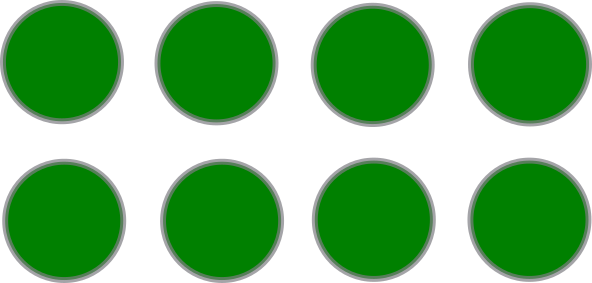
\includegraphics[width=.5\linewidth]{entropy_cluster/step1.png}
			\caption{Free particles. $H=3$}
		\end{subfigure}
		\begin{subfigure}{.5\textwidth}
			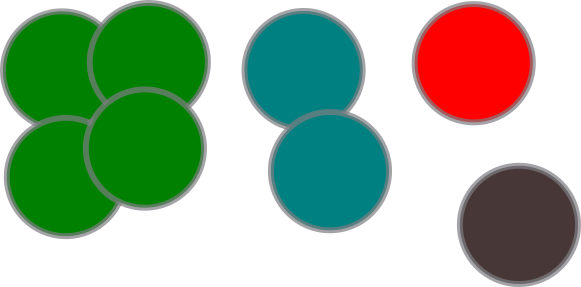
\includegraphics[width=.5\linewidth]{entropy_cluster/step2.png}
			\caption{Some Free and Some Bound Particles.\\ $0 < H < 3$}
		\end{subfigure}
		\begin{subfigure}{.5\textwidth}
			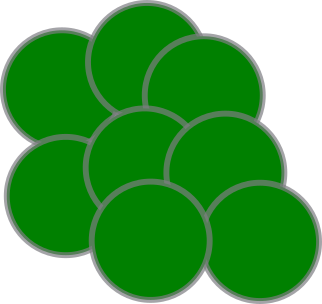
\includegraphics[width=.5\linewidth]{entropy_cluster/step3.png}
			\caption{Bount particles. $H=0$}
		\end{subfigure}
		\caption{entropy of a system of $8$ particles}
	\end{figure}
	

	\subsection{Specific Heat, $C(p,L)$}
	According to the definition of specific heat in thermodynamics \ref{def:specific-heat-thermodynamics}  we can find specific heat if we know the temperature and entropy. In percolation theory we measure the Shannon entropy, $H(p,L)$. And we use $(1-p)$ as the analogue of temperature which gives
	\begin{align}
		C &= (1-p) \frac{dH}{d(1-p)} \\
		  &= -(1-p) \frac{dH}{dp}
		  \label{def:specific-heat-percolation}
	\end{align}
	using this definition we can easily find the specific heat of the percolating system. And from specific heat we obtain the critical exponent $\alpha$.
	
	\subsection{Order Parameter, $P(p,L)$}
		From above discussion we can say that if $p\geq p_c$ the spanning cluster exists but we still cannot say if a randomly chosen site belongs to the spanning cluster. Therefore we need to quantify the strength of the spanning cluster. Percolation strength or $P$ is defined as the probability to find the site that belongs to the spanning cluster, meaning randomly pick a site and what is the probability that the selected site will belong to the spanning cluster. And this quantity should depend on occupation probability $p$ and system size $L$. We call it Percolation Strength or sometimes Order Parameter as it describes the measure of order in the system. Order means the likeliness of not getting confused. If all clusters of same size, i.e. identical, we will get confused which cluster we have chosen ($p=0$ case) but if there is only one cluster there is no chance of confusion ($p=1$ case).\\
		We define the percolation strength as
		\begin{equation}
			P = \frac{\text{number of sites in the spanning cluster}}{\text{total number of sites in the lattice}}
		\end{equation}
		But in a system where there are no boundary, e.g. a network or Bethe lattice, the idea of spanning cluster is not valid. Then we use the largest cluster to define the percolation strength
		\begin{equation}
			P = \frac{\text{number of nodes in the largest cluster}}{\text{total number of nodes in the network}}
		\end{equation}
		Both definition, though looks a bit different when plotted, gives the same critical exponent $\beta$. How to find this exponent is shown in section \ref{subsect:order-parameter}.
		
	    Mathematically
		\begin{align}
			P(p,L) &= \frac{K}{\sum_{i} k_i}
			\label{def:order-parameter}
		\end{align}
		where $K$ is the size of the spanning cluster and $k_i$ is the size of the $i-th$ cluster.
		Percolation strength is the Order parameter of the system which is the measure of Order of a system.
		Note that, with periodic boundary condition we have
		\begin{equation}
			\sum_{i} k_i = L^2
		\end{equation}
		and without periodic boundary condition
		\begin{equation}
			\sum_{i} k_i = L(L-1)
		\end{equation}
		
	
	\subsection{Susceptibility, $\chi(p,L)$}
	\subsection{Mean Cluster Size, S}
	\subsection{Cluster Size Distribution Function, $n_s$} \label{subsect:cluster-size-dist-func}
		\begin{equation}
			n_s(p_c)\sim s^{-\tau}
		\end{equation}
	\subsection{Correlation Function, $g(r)$}		
	\subsection{Correlation length, $\xi$}
	\subsection{Fractal Dimension, $d_f$} \label{subsect:fractal-dim}

\section{Exact Solutions}
	Percolation problem can be solved exactly in $1$ and $\infty$ dimension. In dimension $1 < d < \infty$ there is not analytical solution, it can only be solved approximately using simulations. Analytic solution in dimension greater than $1$ and less than $\infty$ is a still to be solved problem. Interestingly, many of the features found in one dimension seem to be valid for higher dimensions too. Thus using the insight of these exact solutions in $1$ and $\infty$ dimension we get a window into the world of phase transitions, scaling and critical exponents.
	\subsection{One Dimension}
		\subsubsection{Threshold}
		The simplest lattice one can think of is the one dimensional lattice. It consists of many sites arranged at an equidistant positions along a line. Each site of the lattice can either be occupied with probability $p$ or remain empty with probability $1-p$. Thus there are only two possible states of each site.
		\begin{figure}
			\includegraphics[width=\linewidth]{{{1d_lattice}}}
			\caption{One Dimensional Lattice. Empty ones are white and filled ones are black.}
			\label{fig:1d-lattice}
		\end{figure}
		A cluster is a group of neighboring occupied sites which contains no empty sites in between. A single empty sites splits a cluster into two clusters. If we find $n$ successive occupied sites, we say that it forms a cluster of size $n$. We want to find the probability at which an infinite cluster appears for the first time, i.e., the critical occupation probability.\\
		Let $\omega(p,L)$ is the probability that a linear chain of size $L$ has percolating cluster at probability $p$. Note that, if two sites form one cluster, the probability that we find such cluster is $p^2$. Similarly if we want a cluster containing $L$ sites the probability is $\omega(p,L) = p^L$, means $L$ successive sites are occupied independent of each other. 
		\begin{equation}
			\lim_{L \rightarrow \infty} omega(p,L) = 
			\begin{cases}
			  0 \text{ , } \forall p < 1
			  \\
			  1 \text{only if p = 1}
			\end{cases}
		\end{equation}
		For $p=1$ all sites of the lattice are occupied and a percolating cluster spans from $-\infty$ to $\infty$ so that each and every and every sites of the lattice belong to the percolating cluster.For $p<1$ we will have on the average $(1-p)^L$ empty sites. So if $L \rightarrow \infty$, we have $(1-p)^L \rightarrow const.$ revealing that there will be at least one, if not more, empty site somewhere in the chain. Which proves that as long as $p<1$ there is no spanning cluster. Thus the percolation threshold or the critical occupation probability in one dimension is
		\begin{equation}
			p_c = 1
		\end{equation}
		\subsubsection{Cluster Size}
		A cluster of size $s$,a.k.a. $s$-cluster, is formed when $s$ successive sites are occupied and they are surrounded by two empty sites. Probability of $s$ successive sites are being occupied is $p^s$ and $2$ sites are unoccupied is $(1-p)^2$. Thus the probability of picking a cluster at random that belongs to an $s$-cluster is
		\begin{equation}
			n_s = p^s (1-p)^s
			\label{eqn:n_s-1d}
		\end{equation}
		$n_s$ is also the number of $s$-clusters per lattice site. Note that the state of one particular site is independent of any other sites, that's why we multiply probabilities. Further manipulation of equation \ref{eqn:n_s-1d} gives
		\begin{equation}
			n_s = (1-p)^2 \exp (s \ln p) = (1-p)^2 \exp(-s/\xi)
		\end{equation}
		where $\xi$ is the correlation length and defined as
		\begin{equation}
			\xi = -\frac{1}{\ln p} = - \frac{1}{\ln(p_c - (p_c -p))} \sim (p-p_c)^{-1} = (p-p_c)^\nu
			\label{eqn:correlation-length-def}
		\end{equation}
		in the limit $p\rightarrow p_c$ and since $p_c=1$.
		\subsubsection{Mean Cluster Size}
		The probability that an arbitrary site is in $s$-cluster is larger by a factor of s. This site can be any of the sites in the $s$-cluster. The probability that an arbitrary chosen site belongs to a cluster of size $s$ is $n_s s$, since $n_s$ is known to be the number of $s$-clusters per lattice site. Every occupied site must belong to one cluster even if it is a cluster of only one site, i.e., a cluster of size unity.  The probability that an arbitrary site belongs to a cluster is therefore proportional to the probably
		$p$ that it is occupied.
		\begin{equation}
			\sum_{s=1}^{\infty} s n_s = \frac{number of total occupied sites}{number of total lattice sites} = p
			\label{eqn:occupation-probability-in-mean-cluster-size}
		\end{equation}
		A quick check of the validity of equation \ref{eqn:occupation-probability-in-mean-cluster-size} can be performed using equation \ref{eqn:n_s-1d}.
		\begin{align}
			\sum_{s=1}^{\infty}	s n_s \nonumber
			&=  \sum_{s} s (1-p)^2 p^s \nonumber \\
			&= (1-p)^2 \sum_{s} s p^s  \nonumber \\
			&= (1-p)^2 \sum_{s} p \frac{d(p^s)}{dp} \nonumber \\
			&= (1-p)^2 p \frac{d \sum_{s} p^s}{dp} \nonumber \\
			&= (1-p)^2 p \frac{d p(1-p)^{-1}}{dp} \nonumber \\
			&= (1-p)^2 p \left(\frac{1}{1-p} + \frac{p}{(1-p)^2}\right) \nonumber \\
			&= p 
		\end{align}
		Here we have used the series sum \ref{eqn:series-sum-1}.
		\begin{align}
			\sum_s p^s 
			&= p + p^2 + p^3 + \ldots \nonumber \\
			&= p( 1 + p + p^2 + \ldots) \nonumber \\
			&= p(1-p)^{-1}
			\label{eqn:series-sum-1}
		\end{align}
		An important question one can ask is that what is average size of the cluster that we are hitting. Since $n_s s$ is the probability that an arbitrary site belongs to an $s$-cluster and $\sum_{s} n_s s$ is the probability that it belongs to any cluster. Thus we define $w_s$ as
		\begin{equation}
			w_s = \frac{n_s s}{\sum_{s} n_s s}
			\label{eqn:arbitrary-cluster-exactly-s-sites}
		\end{equation}
		$w_s$ is the probability that the cluster to which an arbitrary occupied site belongs contain exactly $s$ sites. The average cluster size $S$ is therefore
		\begin{eqnarray}
			S = \sum_{s} w_s s
		\end{eqnarray}
		This equation is very much similar to
		\begin{equation}
			\bar{x} = \int x p(x) dx
		\end{equation}
		using equation \ref{eqn:arbitrary-cluster-exactly-s-sites} we get
		\begin{align}
			S 
			&= \frac{\sum_{s} n_s s^2}{\sum_{s} n_s s} \nonumber \\
			&= \sum_{s=1}^{\infty} \frac{s^2 n_s}{p} \nonumber\\
			&= \frac{(1-p)^2}{p} \sum_{s=1}^{\infty} s^2 p^s \nonumber \\
			&= \frac{(1-p)^2}{p} \left(p \frac{d}{dp}\right)^2 \left(\sum_{s=1}^{\infty} p^s\right) \nonumber \\
			&= \frac{(1-p)^2}{p} \left(p \frac{d}{dp}\right)^2 (p(1-p)^{-1}) \nonumber \\
			&= p(1-p)^2 \frac{d^2}{dp^2} (p(1-p)^{-1}) \nonumber \\
			&= p(1-p)^2 \frac{d}{dp}(1-p)^{-2} \nonumber \\
			&= p(1-p)^2 2 (1-p)^{-3} \nonumber \\
			&= \frac{2p}{1-p} \nonumber \\
			&= \frac{1 + p}{1 - p}
		\end{align}
		we can write
		\begin{equation}
			S(p) = \frac{1-p}{1 + p} = \frac{p_c + p}{p_c - p}
		\end{equation}
		using the fact that $p_c = 1$ in 1D lattice.
		This equation reveals that the mean cluster size diverges for $p\rightarrow p_c$ where the minus	sign signifies that we are approaching from below $p_c$. This is in sharp contrast with	higher dimensional ones where we can approach to $p_c$ from either end while in one	dimension we cannot have access to the state $p > p_c$ . We thus find the mean cluster	size diverges following power law as we have \cite{nesm-lecture-notes}
		\begin{equation}
			S(p) \sim (p_c - p)^{-1}
		\end{equation}
		We encounter the similar behaviour in the higher dimensions also.
		
		\subsubsection{Correlation Function and Correlation Length}
		The correlation function or pair connectivity $g(r)$ is the probability that a site at position $r$ from an occupied site belongs to the same finite cluster. We are not including the contribution of the infinite cluster. This is valid infinite cluster does not exists as long as $p<1$. Let $r=0$ then $g(r=0)=1$ since the site at $r=0$ is the selected occupied site by definition. For 1D case a site at $r$ to be occupied and belongs to the same finite cluster, we will need $r$ subsequent sites and the probability of getting this is $p^r$. Therefore
		\begin{equation}
			g(r) = p^r
		\end{equation}
		It can also be expressed in terms of correlation length $\xi$
		\begin{equation}
			g(r) = \exp (\ln(p^r)) = \exp(-r/\xi)
		\end{equation}
		where $\xi$ is the correlation length \ref{eqn:correlation-length-def}.\\
		Now that we have correlation function, we can define mean cluster size in terms of it
		\begin{equation}
			S = 1 + \sum_{r=1}^{\infty} g(r)
			\label{eqn:mean-cluster-size-correlation-function}
		\end{equation}
		At this point it is evident that the cutoff cluster size $s_\xi$ , mean cluster size $S(p)$, and correlation length $\xi$ diverges at the percolation threshold. The divergence has the form of a	simple power law of the distance from the critical occupation probability. In higher dimensional percolation problem this observation is also valid.
		
	\subsection{Infinite Dimension}
	Apart from one dimension percolation problem can be solved in infinite dimension. For this we need a suitable playground such as Bethe lattice. Bethe lattice lattice is a special type of lattice  where each site has $z$ neighbors and each branch gives rise to $(z-1)$ other branches. Figure \ref{fig:bethe-lattice} shows the Bethe lattice for $z=3$. Note that for $z=2$ we have nothing but the one dimensional lattice. \subsubsection{Properties of infinite dimensional object}
	For a 3D object the surface area is has dimension to $L^2$ and volume as dimension $L^3$. The same pattern is true of object in any dimension. If we denote area by $A$ and volume by $V$ for any dimension we have
	\begin{equation}
		A \propto V^{1-1/d}
	\end{equation}
	now as $d \rightarrow \infty$ we have
	\begin{equation}
		A \propto V
	\end{equation}
	Therefore if we find that the area of any object is proportional to its volume we can say it is an infinite dimensional object.
	\subsubsection{Bethe Lattice}
	In order to construct Bethe lattice for any $z$ we start with a central point which will be connected to $z$ sites. For example if $z=3$ then we will have a central site connected to $3$ sites by a branch and when we go to next layer each branch will be divided to $2$ more branches and this process will be continued up to $r$ layers \ref{fig:bethe-lattice}. Only at the surface of the lattice, where the branching is stopped, is only one bond or branch connecting the surface site to the interior. There is only open loops in this structure, which means	that if we never change direction always reach new site if we never go back.Number of sites in the Bethe lattice increases exponentially with the distance from the origin, whereas in any $d$-dimensional lattice structure it	would increase with distance $d$ . In the case of Bethe lattice with $z=3$, the origin is surrounded by a shell of three sites ("first generation"), in the second shell we have six sites followed by a third	generation of twelve sites, etc.
	\begin{figure}
		\centering
		\includegraphics[width=10cm]{{{bethe-lattice}}}
		\caption{Bethe Lattice for $z=3$}
		\label{fig:bethe-lattice}
	\end{figure}
	After $r$ generation the total number of sites in the Bethe lattice is
	\begin{equation}
		1+3\times(1 + 2 + \ldots + 2^{r-1}) = 3.2^r - 2
	\end{equation}
	The number $3\times 2^{r-1}$ is the number of sites at the surface.
	Here we have used the following finite series sum
	\begin{equation}
		1+2+2^2+2^3+\ldots+2^r = 2^{r+1} - 1
	\end{equation}
	And if we measure the surface to volume ratio we get
	\begin{equation}
		\frac{A}{V} = \frac{number of sites in the surface}{total number of sites} = \frac{3\times 2^{r-1}}{3\times2^r - 2}
	\end{equation}
	as $r\rightarrow\infty$ we get
	\begin{equation}
		\frac{A}{V} \sim \frac{3\times 2^{r-1}}{3\times2^r} = \frac{1}{2} = constant
	\end{equation}
	Therefore Bethe lattice is indeed an infinite dimensional lattice.
	\subsubsection{Percolation Threshold}
	Percolation threshold of Bethe lattice is the occupation probability at which an infinite cluster appears for the first time. To find it we start walking from the origin and after one step we have $z-1$ new bonds that is connected to $z-1$ new sites in those direction. On the average there will be $(z-1)p$ occupied sites. And for each site there will be another $z-1$ branch and those bonds are connected to $(z-1)p$ sites on the average and so on. After $r$ step we will have an infinite cluster at probability $((z-1)p)^r$. Since $r\rightarrow \infty$ we have $((z-1)p)^r = 0$ if $(z-1)p < 1$. Thus we choose $(z-1)p = 1$ so that we will get an infinite cluster. That lead us to the desired critical  occupation  probability
	\begin{align}
		(z-1)p_c &= 1 \nonumber \\
		p_c 	 &= \frac{1}{z-1}
	\end{align}
	For $z=3$ we have $p_c = 1/2$.
	\subsubsection{Percolation Strength}
	Percolation strength of an infinite cluster is the probability of any arbitrary site to be the part of the infinite cluster. For the sake of calculation, for $p>p_c$ in the Bethe lattice, we introduce a new quantity $Q$ as the probability that an arbitrary site is note connected to the infinite cluster through a fixed branch originating from this site. Restricting ourselves to the lattice with $z=3$ and using basic probability theory, the strength 
	\begin{equation}
		P(p) = p(1-Q^3)
	\end{equation}
	Here $p$ is the probability that the site is occupied and $(1-Q^3)$ is the probability that at least one branch is connected to infinity.\\
	The probability that the two subbranches which start at the neighbor are not both leading infinity is	$Q^2$. The quantity $pQ^2$ is the probability that this neighbor is occupied but not connected to infinity	by any of its two subbranches. This neighbor is empty with probability $(1-p)$, in which case even	well connected subbranches do not help it. This gives us,
	\begin{equation}
		Q = (1-p) + p Q^2
	\end{equation}
	This is the probability that this fixed branch does not lead to infinity, either because the connection	is already broken at the first neighbor, or because later something is missing in the subbranch. So the solution of this quadratic equation is
	\begin{equation}
		Q = 1, \frac{1-p}{p}
	\end{equation}
	For $z$ neighbors, in general we have
	\begin{equation}
		Q = 1, 1 - \frac{2p(z-1)-2}{p(z-1)(z-2)}
	\end{equation}
	for $p<p_c$, there are no infinite clusters, fo with probability $1$ there are no connection to infinity. Now we use Taylor expansion for $P(p)$ around $p=p_c=1/2$
	\begin{align}
		P(p) = 
		\begin{cases}
		0	&\text{ for } p < p_c \\
		p\left(1- \left(\frac{1-p}{p}\right)^3\right) &\text{ for } p \geq p_c
		\end{cases}
	\end{align}
	Let,
	\begin{equation}
		f(p) = \left(\frac{(1-p)}{p} \right)^3
	\end{equation}
	Then
	\begin{align}
		f^\prime(p) &= -3p^-4 (1-p)^3 - 3 p^-3 (1-p)^2 \nonumber \\
		&= -\frac{3}{p} \left(\frac{(1-p)}{p}\right)^3 -\frac{3}{p} \left(\frac{(1-p)}{p}\right)^2
	\end{align}
	\begin{align}
		P(p) &= P(p_c) + (p-p_c) P^\prime(p_c) + \ldots \\
		&= 0 + (p-p_c) \left(1-f(p_c) - p f^\prime(p_c)\right) + \ldots \\
		&= 6(p-p_c) + \ldots \\
	\end{align}
	Therefore we get
	\begin{equation}
		P(p) \propto (p-p_c) \ \text{for} p \rightarrow p_c^+
	\end{equation}
	the critical exponent $\beta$ is defined by
	\begin{equation}
	P(p) \propto (p-p_c)^\beta
	\end{equation}
	Thus in Bethe lattice $\beta = 1$.
	\subsubsection{Mean Cluster Size}
	In case of Bethe lattice the mean cluster size is defined as the average number of sites to which the origin belongs. Let $T$ be the mean cluster size for one branch, that is the average number of sites to which the origin is connected and which belongs to one branch. Again, subbranches have the same mean cluster $T$ as the branch itself. If the neighbor is empty the cluster size for this branch is zero. If the neighbor is occupied, it contributes its own mass to the cluster which is unity and adds the mass $T$ for each of its two subbranches. Thus,
	\begin{equation}
		T = (1-p) \times 0 + p(1+2T)
	\end{equation}
	Solving this we get
	\begin{equation}
		T = \frac{p}{1 - 2p}
	\end{equation}
	for $p<p_c$. \\
	The total cluster size is zero if the origin is empty and $(1+3T)$ if the origin is occupied. Therefore the mean cluster size $S(p)$ is
	\begin{align}
		S(p) &= 1 + 3 T \\
		     &= \frac{1+p}{1-2p} \nonumber\\
   		     &= \frac{1+p}{2(p_c-p} \nonumber \\
   		     &=\frac{1+p}{2} (p_c - p)^{-1}
	\end{align}
	Thus the critical exponent $\gamma = 1$ for Bethe lattice. This is the exact result for mean cluster size and we notice that it diverges for $p\rightarrow p_c$.
	\subsubsection{Correlation Function and Correlation Length}
	The radial correlation function $g(r)$ is the average number of occupied sites within the same cluster at a distance $r$ from an arbitrary occupied site. The probability that a site at distance $r$ from the origin is occupied and the sites in between are occupied too is equal to $p^r$. Now if we think about a shell of radius $r$ then the number of all the sites enclosed by this shell is $z(z-1)^{r-1}$. Thus
	\begin{align}
		g(r) &= z(z-1)^{r-1} p^r \\
			 &= \frac{z}{z-1} \left(p(z-1)\right)^r \\
			 &= \frac{z}{z-1} \exp \left[\log\left[p(z-1)\right]\right]
	\end{align}
	The value of percolation threshold for Bethe lattice can be found by analyzing the behaviour of the correlation function at large distances, i.e. at r $\rightarrow \infty$. For $p(z-1) < 1$, $g(r)$ decreases exponentially, on the other hand for $p(z-1)>1$, the correlation function diverges which signifies the existence of an infinite cluster. Mathematical treatment yields the correlation length from \ref{eqn:correlation-length-def}
	\begin{align}
		\xi &= \frac{-1}{\log[p(1-z)]} \nonumber \\
			&= \frac{-1}{\log(p/p_c)} \nonumber \\
			&= (p-p_c)^{-1}
	\end{align}
	as $p$ approaches $p_c$, that is $\nu = 1$. \\
	Clearly the 1D lattice and Bethe  lattice exhibits power law while we approach a critical value which suggests the same phenomena in other variants of such problems.

\section{Algorithm} \label{sect:algorithm}
In the classical Hosen-Kopelman algorithm for percolation model \cite{Hoshen1976}, one first choose an occupation probability $p$ and then generate a number $r$ for each site of the lattice. The site is occupied if $r \leq p$ and remain empty if $r > p$. One therefore create an entire new state of a given lattice size for every different value of $p$. Note that the number of occupied sites $n$ for a given $p$ may very in each realization. However, the expected or ensemble average over $M$ experiments will give $n = p M$ in the limit $M \rightarrow$. Thus the number of occupied bonds or sites is also a measure of $p$. Using this idea Ziff and Newman \cite{Newman2001} proposed an algorithm which generate states for each value of $n$ from zero up to some maximum value $n = L^2$ for site percolation on $L\times L$ square lattice for instance. In this way, one can save some effort by noticing the fact that a new state with $n + 1$ occupied sites or bonds can be created by adding one extra randomly chosen site or bond to the state containing n sites or bonds. The first step of their algorithm is to decide an order in which the bonds or sites are to be occupied. That is, every attempt to occupy a bond/site is successful.

\section{Relation of Phase Transition with Percolation}

\section{Application}\label{sect:application}
	Ever since the percolation phenomena was discovered it has been extensively used in wide range of science. Some of it is discussed here. Though limited, this discussion gives us the significance of percolation and enables us to appreciate it.
	\subsection{Epidemiology}
	Many diseases spread through human populations via close physical interactions. The interpersonal contact patterns that underlie disease transmission can naturally be thought to form a network, where links join individuals who interact with each other. During an outbreak, disease then spreads along these links. All epidemiological models make assumptions about the underlying	network of interactions, often without explicitly stating them.
	
	Percolation has long been an important tool in infectious disease epidemiology \cite{Bansal2007}. L Meyers gave a wonderful insight of contact	network epidemiology, a more powerful approach that applies bond percolation on random graphs	to model the spread of infectious disease through heterogeneous populations \cite{Meyers2006}.
	
	Before that	in 2000, Moore et al. studied some simple models of disease transmission on small-world networks \cite{Moore2000}. They showed that the resulting models display epidemic behavior when the infection	or transmission probability rises above the threshold for site or bond percolation on the network,	and they gave exact solutions for the position of this threshold in a variety of cases. 
	
	Alessandro	Vespignani and his team studied wifi networks and malware epidemiology. They developed an	epidemiological model that takes into consideration prevalent security flaws on these routers.They	simulated spread of such a contagion on real-world data for georeferenced wireless routers \cite{Hu2009}.
	
	Sander et al. considered a spatial model related to bond percolation for the spread of a disease that	includes variation in the susceptibility to infection. They worked on a lattice with random bond	strengths and showed that with strong heterogeneity, i.e. a wide range of variation of susceptibility, patchiness in the spread of the epidemic is very likely, and the criterion for epidemic outbreak	depends strongly on the heterogeneity. Their results were qualitatively different from those of standard models in epidemiology, but correspond to real effects \cite{Sander2002}.
	
	After the birth of scale free	network the study of epidemics has become even more popular among statistical physicists.
	
	
	\subsection{Neural Network and Cognitive Psychology}
	Percolation is used to understand the way activation and diffusion of neural activity occur within neural networks \cite{Friedenberg2011}. Iian Breskin's team in 2006 studied living neural networks by measuring the neurons' response to a global electrical stimulation. They showed through analysis that neural connectivity is lowered by reducing the synaptic strength, chemically blocking neurotransmitter receptors. They used a graph-theoretic approach to show that the connectivity undergoes a percolation transition. This occurs as the giant component disintegrates, characterized by a power law with an exponent $\beta \simeq 0.65$	 \cite{Breskin2006}.\\
	
	It is easiest to understand percolation theory by explaining its use in epidemiology \cite{Moore2000}. Individuals that are infected with a disease can spread it knowingly or unknowingly via social or physical interaction. It's easy to say that the more social a person is the more it is likely that he will spread more disease than the unsocial one. Therefore some factors, e.g., occupation, size of social circle etc, influence the rate of infection. \\
	
	
	Now, if one were to think of neurons as the individuals and synaptic connections as the social bonds between people, then one can determine how easily	messages between neurons will spread \cite{Friedenberg2011} When a neuron fires, the message is transmitted along	all synaptic connections to other neurons until it can no longer continue.
	
	 Synaptic connections are	considered either open or closed (like a social or unsocial person) and messages will flow along	any and all open connections until they can go no further. Just like occupation and sociability play	a key role in the spread of disease, so does the number of neurons, synaptic plasticity \cite{Hughes1958} and	long-term potentiation when talking about neural percolation. Percolating clusters are a single large	group of neurons that are all connected by open bonds and take up the majority of the network.	Any signals that originate at any point within the percolating cluster will have a great impact and	diffusion across the network than signals that original outside of the cluster.
	  This is much like	how a teacher is more likely to spread an infection to a whole community through contact with the	students and subsequently with the families than an isolated businessman that works from home.
	
	
	\subsection{Ferromagnetism}
	One of the most studied phase transition phenomena of physics is that para-magnetic to ferromagnetic transition. The magnetic spins of a magnetic material, e.g., nickel, interact with each other:	the energy is lower if the two spins on adjacent nickel atoms are parallel than if they are anti-parallel. This lower energy tends to cause the spins to be parallel and below a temperature called	the Curie temperature,$T_c$ , most of the spins in the nickel are parallel, their magnetic moments then	add up constructively and the piece of nickel has a net magnetic moment: it is a ferromagnetic.
	 Above the Curie temperature on average half the spins point in one direction and the other half in	the opposite direction. Then their magnetic moments cancels out, and the nickel has no net magnetic	moment. It is then a para-magnet. Thus at $T_c$ the nickel goes from having no magnetic moment to	having a magnetic moment. This is a sudden qualitative change and when this happens we say that	a phase transition has occurred. Here the phase transition occurs when the magnetic moment goes	from zero to non-zero. It is from the para-magnetic phase to the ferromagnetic phase.	So, this critical value $T_c$ of the temperature marking the borderline between the existence and	non-existence of so called spontaneous magnetization. A standard mathematical model for this	phenomenon is the Ising model \cite{Cipra1987}. It turns out that there are two parameters which specify	the conditional probabilities: the 'external magnetic field' $h$, and the strength $J$ of interaction	between neighbors. If $J = 0$, the states of different vertices are independent, and the process is	equivalent to site percolation \cite{Coniglio1976}. The relationship between the Ising model and bond percolation	is rather strong. It turns out that they are linked via a type of 'generalized percolation' called the other considerations \cite{Coleman1992, Seiden1990}. 
	 Studing the random-cluster model,
	 one can obtain conclusions valid simultaneously for percolation and the Ising model.
	 This discovery was made in 1970 by Fortuin and Kastelyn \cite{Fortuin1972a, Fortuin1972b, Fortuin1972c}, and it has
	 greatly influenced part of the current view of disordered physical systems
	 
	 
	\subsection{Cosmology}
	We know mass distribution and motions of the components of a galaxy are determined by gravity,	it has not been clear what is responsible for the striking morphology of a spiral galaxy such as	shown in the figure.
	\begin{figure}
		\centering
		\includegraphics[width=10cm]{{{galaxy}}}
		\caption{NGC $4414$, a typical spiral galaxy in the constellation Coma Berenices, is about $55,000$ light-years in diameter and approximately $60$ million light-years away from Earth.}
		\label{galaxy}
	\end{figure}
	 The spiral arms extend over 16,000 parsecs (1 parsecs equals 3.26 light-years), and the traditional view is that it is necessary to have a long-range interaction like gravity, which interacts with object that have mass,	to create such long-range order. However, in condensed matter physics it is well known that long-range order can be induced by a short-range interaction, and this is a characteristic feature of a	continuous phase transition [48].
	 
	The structural features of spiral galaxies arises from a percolation phase transition that underlies the phenomenon of propagating star formation. According to this	view, the appearance of spiral arms is a consequence of the differential rotation of the galaxy	and the characteristic divergence of correlation lengths for continuous phase transitions.
	
	 Other	structural properties of spiral galaxies, such as the distribution of the gaseous components and the	luminosity, arise directly from a feedback mechanism that pins the star formation rate close to the	critical point of the phase transition. At least for some galaxies, morphological and other features	are already fixed by general properties of phase transitions, irrespective of detailed dynamic or	other considerations \cite{Seiden1990, Coleman1992}.
	
	
	
Definitions of some quantities used in percolation.
Basic Algorithm
\subsection{Square Lattice}
		A square lattice is an ideal playground for percolation. If it has length $L$ then number of sites in the lattice is $L^2$ and number of bonds in the lattice is $2 L^2$. All sites are equally separated from each other at a certain distance. And all sites have exactly four neighbor. Since with the periodic boundary condition the sites in the left edge are connected with the sites in the right edge and same rule for sites in the top and bottom edges. If the sites are densely spaced the experiment will be accurate, meaning, the larger the size of the lattice the accurate the results will be. It implies that a lattice of infinite size should be used which is practically impossible. The simple solution to this problem is to use number of large lengths, (say $L = \{L_1, L_2, \ldots L_n \}$, where $n$ is a finite number and $L_1 < L_2 < \ldots < L_n$), and extrapolate the results for infinite lattice. The visual structure of the square lattice is as follows \ref{fig:sq_lattiec_empty}. This is and empty lattice structure. Filled circles are for occupied site and filled bonds are for occupied bonds \ref{fig:site_bond_symbol}.

	\begin{figure}[htbp]
		\centering
		\includegraphics{{{square_lattice_5}}}
		\caption{Square Lattie (empty) of length 6}
		\label{fig:sq_lattiec_empty}
	\end{figure}

	\begin{figure}
		\begin{subfigure}{.5\textwidth}
			\centering
			\includegraphics[width=.1\linewidth]{{{site_empty}}}
			\caption{Empty Site}
		\end{subfigure}
		\begin{subfigure}{.5\textwidth}
			\centering
			\includegraphics[width=0.1\linewidth]{{{site_occupied}}}
			\caption{Occupied Site}
		\end{subfigure}
		\begin{subfigure}{.5\textwidth}
			\centering
			\includegraphics[width=.1\linewidth]{{{bond_empty}}}
			\caption{Empty Bond}
		\end{subfigure}
		\begin{subfigure}{.5\textwidth}
			\centering
			\includegraphics[width=.1\linewidth]{{{bond_occupied}}}
			\caption{Occupied Bond}
		\end{subfigure}
		\caption{Site and Bond symbol (empty and occupied).}
		\label{fig:site_bond_symbol}
	\end{figure}

\subsection{Site Percolation}
	The algorithm for site percolation is as follows,
	\begin{enumerate}
		\item take a square lattice of length $L$.
		\item fill all $2 L^2$ bonds initially.
		\item occupy a randomly chosen site and it will join some clusters.
		\item each time a site is occupied, it will get connected to four neighboring bonds and will form a cluster of size $4$. Note that we define cluster size by number of bonds in it.
		\item if a site is occupied and right next to it there is another occupied site and a cluster of size $7$ will be formed.
		\item this process is repeated until all the sites are occupied and only one cluster remains
	\end{enumerate}
	The formation of cluster is visualized in the figure \ref{fig:cluster_growth_site_percolation}.

	\begin{figure}
		\begin{subfigure}{.5\textwidth}
			\centering
			\includegraphics[width=.8\linewidth]{{{sq_lattice_site_percolation_1_0}}}
			\caption{Initial state}
		\end{subfigure}
		\begin{subfigure}{.5\textwidth}
			\centering
			\includegraphics[width=.8\linewidth]{{{sq_lattice_site_percolation_1_1}}}
			\caption{Iteraion 1}
		\end{subfigure}
		\begin{subfigure}{.5\textwidth}
			\centering
			\includegraphics[width=.8\linewidth]{{{sq_lattice_site_percolation_1_2}}}
			\caption{Iteraion 2}
		\end{subfigure}
		\begin{subfigure}{.5\textwidth}
			\centering
			\includegraphics[width=.8\linewidth]{{{sq_lattice_site_percolation_1_3}}}
			\caption{Iteraion 3}
		\end{subfigure}
		
		\caption{Growth of a Cluster in Site Percolation on square Lattice}
		\label{fig:cluster_growth_site_percolation}
	\end{figure}
		
\subsection{Bond Percolation}
The algorithm for bond percolation is as follows,
\begin{enumerate}
	\item take a square lattice of length $L$.
	\item fill all $L^2$ the sites initially.
	\item occupy a randomly chosen bond and it will join some clusters.
	\item each time a bond is occupied, it will get connected to two neighboring sites and will form a cluster of size $2$. Here cluster size by number of sites in it.
	\item if a bond is occupied and right next to it there is another occupied bond and they are connected by a site and a cluster of size $3$ will be formed.
	\item this process is repeated until all the bonds are occupied and only one cluster remains
\end{enumerate}
The formation of cluster is visualized in the figure \ref{fig:cluster_growth_bond_percolation}.
	\begin{figure}
		\begin{subfigure}{.5\textwidth}
			\centering
			\includegraphics[width=.8\linewidth]{{{sq_lattice_bond_percolation_1_0}}}
			\caption{Initial state}
		\end{subfigure}
		\begin{subfigure}{.5\textwidth}
			\centering
			\includegraphics[width=.8\linewidth]{{{sq_lattice_bond_percolation_1_1}}}
			\caption{Iteraion 1}
		\end{subfigure}
		\begin{subfigure}{.5\textwidth}
			\centering
			\includegraphics[width=.8\linewidth]{{{sq_lattice_bond_percolation_1_2}}}
			\caption{Iteraion 2}
		\end{subfigure}
		\begin{subfigure}{.5\textwidth}
			\centering
			\includegraphics[width=.8\linewidth]{{{sq_lattice_bond_percolation_1_3}}}
			\caption{Iteraion 3}
		\end{subfigure}
		\caption{Growth of a Cluster in Bond Percolation on square Lattice}
		\label{fig:cluster_growth_bond_percolation}
	\end{figure}
		
	

	
%!TEX root = ../thesis.tex
%*******************************************************************************
%****************************** Fifth Chapter **********************************
%*******************************************************************************
\chapter{Ballistic Deposition on Square Lattice}
\label{chapter:ballistic-deposition}
% **************************** Define Graphics Path **************************
\ifpdf
    \graphicspath{{Chapter4/Figs/}{Chapter5/Figs/}{Chapter5/Figs/L0/}{Chapter5/Figs/L1/}{Chapter5/Figs/L2/}{Chapter5/Figs/traditional/}}
\else
    \graphicspath{{Chapter4/Figs/}{Chapter5/Figs/}{Chapter5/Figs/L0/}{Chapter5/Figs/L1/}{Chapter5/Figs/L2/}Chapter5/Figs/traditional/}
\fi


We investigate percolation by random sequential ballistic deposition (RSBD) on a square lattice with interaction range upto second nearest neighbors. The critical points $p_c$ and all the necessary critical exponents $\alpha$, $\beta$, $\gamma$, $\nu$ etc. are obtained numerically for  each range of interactions. Like  in its thermal counterpart, we find that the critical exponents of RSBD depend on the range of interactions and for a given range of interaction they obey the Rushbrooke inequality. Besides, we obtain the exponent $\tau$ which characterizes the cluster size distribution  function $n_s(p_c)\sim s^{-\tau}$ \ref{subsect:cluster-size-dist-func} and the fractal dimension $d_f$ that characterizes the spanning cluster at $p_c$ \ref{subsect:fractal-dim}. Our results suggest that the RSBD for each range of interaction belong to a new universality class which is in sharp contrast to earlier results of the only work that exhist on RSBD.
\\
Imagine a spherical shaped object, say marble, is thrown on top of a 2D square lattice structure. First possible scenario is that the marble will be deposited in the first encountered site in the lattice . Now if the first encountered site is not empty, the possible scenario is that the marble will go in any of the four direction, $+x$, $-x$, $+y$ or $-y$, assuming no other direction in between is allowed in the lattice.  Now if the first neighbor is not empty then the marble will continue to go on in the previously selected direction and choose the next neighbor. This is the main theme of this thesis.\\
In our experiment, we occupy a randomly chosen site if it is empty else we select one of its four neighbor to occupy if it is empty else select next neighbor in that direction and occupy that site if it is empty else ignore current iteration and choose another site randomly. This process is repeated until there is no empty site in the lattice. We call this process the ballistic deposition on the square lattice. We introduce 1st and 2nd nearest neighbor interaction in this way.



\section{Redefinition of Site Percolation}
	In site percolation we take a square lattice of length $L$ and we choose sites randomly and occupy them and measure cluster size with the number of site in a cluster. This is the traditional definition of site percolation.
	
	First let us discuss about two most important quantities of interests in the		theory of phase transition and critical phenomena are the		entropy $H$ and the order parameter $P$ since they are the		ones which define the order of transition. For instance,		in the first order transition there must be a jump or gap		in entropy at the critical point which is why first order 		transition requires latent heat. Similarly, the order parameter too must suffer a jump or discontinuity at the		critical point and that is the reason why in the first order transition new and old phase can coexist at the same		time. Besides, they are also used as a litmus test to		check whether the transition is accompanied by symmetry breaking or not. In the case of symmetry breaking,		the system undergoes a transition from the disordered		state, which is characterized by maximally high entropy,		to the ordered state, which is characterized by maximally		high order parameter. Such transition happens with an		abrupt or sudden change in $P$ and $H$ but without gap	or discontinuity at $p_c$.	
	\subsection{The problem with the old definition}
		If we use the traditional definition of site percolation we encounter some serious problem. Firstly, it violates the second law of thermodynamics which states entropy cannot decrease in a closed system \cite{Benguigui2013} which is discussed in section \ref{subsect:entropy-thermodynamics}. But the traditional definition gives a graph of entropy where entropy is zero at $p=0$ then entropy increases to a maximum value and again decreases to zero at $p=1$. Figure \ref{fig:entropy-traditional} show the graph of entropy using the traditional definition of site percolation. Although ignoring the part where $p \sim 0$ gives us the correct exponent from the derivative of entropy (specific heat) but it surely violates one of the fundamental laws of physics.
		\begin{figure}
			\captionsetup[subfigure]{width=0.9\textwidth}
			\begin{subfigure}{0.5\textwidth}
			\centering
			\includegraphics[width=7cm]{{{sq_lattice_site_percolation_periodic__entropy_by_site_-entropy}}}
			\caption{Entropy from the traditional definition of site percolation}
			\label{fig:entropy-traditional}				
			\end{subfigure}
			\begin{subfigure}{0.5\textwidth}
			\centering
			\includegraphics[width=7cm]{{{sq_lattice_site_percolation_periodic__entropy_by_site-entropy-order_parameter-traditional2-L400}}}
			\caption{Entropy from the traditional definition of site percolation}
			\label{fig:order-disorder-transition}
			\end{subfigure}
			\caption{Effect of traditional definition of site percolation}
		\end{figure}
		
		Secondly, it give raise to ambiguity at $p=0$. 		 We know phase transition is an order-disorder transition and system goes from ordered state to disordered state or vice versa. Therefore a system cannot be in both ordered state and disordered state at the same time. But the traditional definition of site percolation does not agree with this. We can see this in figure \ref{fig:order-disorder-transition} where normalized entropy and order parameter is plotted together. We can see that at $p=0$entropy, which represents disorder, is minimum  and order parameter, which represents order, is also zero. Thus the system is in both ordered and disordered state at  the same time. Which is a serious problem with the traditional definition of site percolation.
		
	\subsection{Solution to the problem}
		Our problem will be resolved if the entropy is maximum at $p=0$ and gradually decrease to minimum and order parameter is minimum at $p=0$ and gradually increase to maximum. Since bond percolation does not raise this problem, a closer look at it and comparing it with site percolation is the first thing to do.
		\subsubsection{Bond Percolation}
		 In bond percolation we occupy bond and measure occupation probability by the fraction of the occupied bond with respect to total number of bonds. And we measure cluster size with the number of sites in it. Here, in the initial state, there is no bond present but all the sites are. We simply occupy bonds to connect sites to form clusters. Thus initially all the clusters are of size $1$ (contains exactly one site) giving maximum entropy and minimum order parameter. 
		
		 The algorithm for bond percolation is as follows,
		 \begin{enumerate}
		 	\item take a square lattice of length $L$.
		 	\item fill all $L^2$ the sites initially.
		 	\item occupy a randomly chosen bond and it will join some clusters.
		 	\item each time a bond is occupied, it will get connected to two neighboring sites and will form a cluster of size $2$. Here cluster size by number of sites in it.
		 	\item if a bond is occupied and right next to it there is another occupied bond and they are connected by a site and a cluster of size $3$ will be formed.
		 	\item this process is repeated until all the bonds are occupied and only one cluster remains
		 \end{enumerate}
		 The formation of cluster is visualized in the figure \ref{fig:cluster_growth_bond_percolation}.
		 \begin{figure}
		 	\begin{subfigure}{.5\textwidth}
		 		\centering
		 		\includegraphics[width=.8\linewidth]{{{sq_lattice_bond_percolation_1_0}}}
		 		\caption{Initial state}
		 	\end{subfigure}
		 	\begin{subfigure}{.5\textwidth}
		 		\centering
		 		\includegraphics[width=.8\linewidth]{{{sq_lattice_bond_percolation_1_1}}}
		 		\caption{Iteraion 1}
		 	\end{subfigure}
		 	\begin{subfigure}{.5\textwidth}
		 		\centering
		 		\includegraphics[width=.8\linewidth]{{{sq_lattice_bond_percolation_1_2}}}
		 		\caption{Iteraion 2}
		 	\end{subfigure}
		 	\begin{subfigure}{.5\textwidth}
		 		\centering
		 		\includegraphics[width=.8\linewidth]{{{sq_lattice_bond_percolation_1_3}}}
		 		\caption{Iteraion 3}
		 	\end{subfigure}
		 	\caption{Growth of a Cluster in Bond Percolation on square Lattice}
		 	\label{fig:cluster_growth_bond_percolation}
		 \end{figure}
		
		
		Keeping this in mind one might guess the possible rule for site percolation. We should have a lattice of $2 L^2$ bonds and no sites and we should occupy site and connect bonds with sites to form clusters. As usual the occupation probability will be measured by $n/L^2$ where $n$ is the number of occupied sites. In this way we have maximum entropy and minimum order parameter at $p=0$ see figure \ref{fig:ordered-disordered-transition}.
		
		\subsubsection{Site Percolation}
		The algorithm for site percolation is as follows,
		\begin{enumerate}
			\item take a square lattice of length $L$.
			\item fill all $2 L^2$ bonds initially.
			\item occupy a randomly chosen site and it will join some clusters.
			\item each time a site is occupied, it will get connected to four neighboring bonds and will form a cluster of size $4$. Note that we define cluster size by number of bonds in it.
			\item if a site is occupied and right next to it there is another occupied site and a cluster of size $7$ will be formed.
			\item this process is repeated until all the sites are occupied and only one cluster remains
		\end{enumerate}
		The formation of cluster is visualized in the figure \ref{fig:cluster_growth_site_percolation}.
		
		\begin{figure}
			\begin{subfigure}{.5\textwidth}
				\centering
				\includegraphics[width=.8\linewidth]{{{sq_lattice_site_percolation_1_0}}}
				\caption{Initial state}
			\end{subfigure}
			\begin{subfigure}{.5\textwidth}
				\centering
				\includegraphics[width=.8\linewidth]{{{sq_lattice_site_percolation_1_1}}}
				\caption{Iteraion 1}
			\end{subfigure}
			\begin{subfigure}{.5\textwidth}
				\centering
				\includegraphics[width=.8\linewidth]{{{sq_lattice_site_percolation_1_2}}}
				\caption{Iteraion 2}
			\end{subfigure}
			\begin{subfigure}{.5\textwidth}
				\centering
				\includegraphics[width=.8\linewidth]{{{sq_lattice_site_percolation_1_3}}}
				\caption{Iteraion 3}
			\end{subfigure}
			
			\caption{Growth of a Cluster in Site Percolation on square Lattice}
			\label{fig:cluster_growth_site_percolation}
		\end{figure}
	
	
	
		 Thus we can give the definition of site(bond) percolation. Take a square lattice of length $L$ with $L^2$ sites and $2L^2$ bonds. In site(bond) percolation all the bonds(sites) are present initially and occupy sites(bonds) to connect bonds(sites) in order to form cluster. Measure occupation probability as a fraction of sites(bonds) with respect to total sites(bonds) \cite{redefinition-of-site-percolation}.
		 
	\subsection{Impact of the new definition}
		The new definition resolves the problems of the traditional definition of site percolation. It does not violet the second law of thermodynamics. Which means that initially at $p=0$ the entropy is maximum and the order parameter is minimum. As we occupy sites and form clusters the entropy decreases. At the critical point the rate of decreasing entropy is maximum. At $p=1$, when all the sites are occupied, there exists only one cluster giving minimum entropy and maximum order parameter \ref{fig:entropy}.		Thus ambiguity of being in ordered and disordered state at the same time is resolved \ref{fig:order-disorder-transition}. Also the critical exponents are unchanged by the new definition. Thus site and bond percolation belong to a universality class \cite{Hassan2015, Hassan2016}.


\section{Structure and Algorithm}
Random percolation (RP) model can also be seen as a random sequential adsorption (RSA) process of particles on a given substrate to form monolayers of clusters of complex shape and structures. In RSA, a site is first picked at random and it is occupied if it is empty and the trial attempt is rejected if it is already occupied. We shall first show that this process too reproduce all the existing results of the CRP including the $p_c$ value. We can modify the rejection criterion. First, we assume that the adsorbing particles are hard sphere and impenetrable. Then we assume that if a particle fall onto an already adsorbed particle it is not straightaway rejected. Instead, it is allowed to roll down over the already deposited particle to one of its nearest neighbours at random following the steepest descent path. The particle is then adsorbed permanently if the nearest neighbour is empty else the trial attempt is rejected. This is known as the ballistic deposition (BD) model for $l = 1$. We also consider the case that if the nearest neighbour is occupied then the incoming particle attempt to push the neighbour to its next neighour site along the same line to make room for itself. However, the trial attempt of pushing the neighbour is successful if the next neibhouring site along the same line is empty else the trial attempt is discarded. We regard it as BD model for $l = 2$ while the classical percolation correspond to BD model with $l = 0$. Our primery goal is to prove that the critical exponents of percolation changes as changes as we increase the range of interaction like we find in its thermal counterpart. We numerically find the various necessary critical exponents and find that BD for each different range of interaction belong to different universality class and each universality class
obeys the Rusbrooke inequality.\\

Percolation is all about configuration of clusters of deposited particles and the investigation of the emergence of a large-scale connected path created by clusters formed by contiguous diposoted particles. We use extensive Monte Carlo simulation on a square lattice with the usual periodic boundary condition to study site percolation according to RSBD rule.\\

The algorithm of the percolation by RSBD can be described as follows. We first label all the sites
row by row from left to right starting from the top left corner. That is, we first label the first row from
left to right as $i=1,2,...,L$, the second row again from left to right as $i=L+1,L+2,....,2L$
and we continue this till we reach the bottom row which we label as $i=(L-1)L+1,...,L^2$. 
Then at each step we pick a discrete random number $R$ from $1,2,...,L^2-1,L^2$ using uniform random number
generator and check if the site it represents is already occupied or not. If it is
empty we occupy it straightaway and move on to the next step. Else we pick one of its neighbours at random. 
The second attempt in the same step, that mimic the roll over mechanism, is successul if the neighbour
it picks is empty and if not the trial attempt to deposit is rejected permanently and we move on to the next 
step anyway. This process is
repeated over and over again till we want it to stop. We call it RSBD of degree one. We also consider
the case of RSBS of degree two where the trial attempt is made to occupy the second nearest neighbour too.
In this case if the incoming particle that fall onto an already occupied site and find its 
neighbour is ocupied too but the next nearest neighbour site is empty then the neighbour move to the empty
site to make space for the incoming perticle to be deposited there. 
\begin{enumerate}
	\item take a square lattice of length $L$.
	\item choose a site randomly
	\item if the chosen site is empty then occupy it else choose one of the four neighbor randomly
	\item if the chosen neighbor is empty then occupy it else choose second nearest neighbor in that direction
	\item if the second nearest neighbor is empty then occupy the site else ignore this step
\end{enumerate}


\section{Finding Numerical Values} 
\label{sect:finding-numerical-values}
	\subsection{Critical occupation probability, $p_c$} 
	\label{subsect:finding-pc}
	When we occupy sites of the square lattice, initially, there are only cluster of size $1$. As we keep occupying different size of clusters starts to appear. At a certain point a special cluster appears which spans the entire lattice. We call this cluster the \textit{Spanning Cluster}. It should be noted that the spanning cluster is a special property of the lattice and the appearance of the spanning cluster is the result of phase transition. At the point where the spanning cluster first appears is called the critical point and denoted by $p_c$, meaning the occupation probability at the critical point. The figure \ref{fig:spanning-probability} shows the graph of the spanning probability, $w(p,L)$, versus the occupation probability $p$ for different interactions ($L0, L1, L2$) for different lengths. We have found that $p_c$ is $0.5927, 0.5782, 0.5701$ for $L0, L1, L2$ respectively.Thus for long range interaction $p_c$ is smaller than for short range interaction. 
		\begin{figure}
			\begin{subfigure}{0.329\textwidth}
				\centering
				\includegraphics[width=\linewidth]{{{sq_lattice_site_percolation_periodic_-occupation_probability-pc0.5927}}}
				\caption{L0}
			\end{subfigure}
			\begin{subfigure}{0.329\textwidth}
				\centering
				\includegraphics[width=\linewidth]{{{sq_lattice_site_percolation_ballistic_deposition_L1_periodic_-occupation_probability-pc0.5782}}}
				\caption{L1}
			\end{subfigure}
			\begin{subfigure}{0.329\textwidth}
				\centering
				\includegraphics[width=\linewidth]{{{sq_lattice_site_percolation_ballistic_deposition_L2_periodic_-occupation_probability-pc0.5701}}}
			\caption{L2}
			\end{subfigure}
			\caption{Spanning Probability, $w(p,L)$ vs Occupation Probability, $p$}
			\label{fig:spanning-probability}
		\end{figure}
	The quantity $w(p, L)$ is called the spanning probability in a non periodic case and wrapping probability in a periodic case.
	The question is how do we find the wrapping probability, given that we have a list of $p_c$ for different length. Note that for a certain length $L$, in each realization the $p_c$ is not exact value, instead it is a range of values that contains the $p_c$. For example, say we have a lattice of length $200$ and for that we will have different $p_c$ at each realization. After an infinite number of experimentation we will have to take an average and that will give the exact value of $p_c$. But since it is practically impossible, we can find $p_{c_{avg}}$ for different lattice size then from the graph we can extrapolate the exact value of $p_c$ for infinite lattice. Here $p_{c_{avg}}$ is calculated from a finite set of $p_c$ for a certain length. This process is not good enough. Since it requires  $p_{c_{avg}}$'s for a number of lattice size which is very costly to obtain. But from the data, list of $p_c$'s for different length, we can find the cumulative frequency distribution. It is astonishing  that for all length the wrapping probability coincide at a specific point. This implies that if we could have an infinite system, the wrapping probability for that system would have gone through this same point. This means we got our critical point, $p_c$, as the intersection of the $w(p,L)$ for different lengths.
	\subsection{Spanning Probability and finding $1/\nu$} \label{subsect:spanning-probability-and-one-by-nu}
	From the figure \ref{fig:spanning-probability} we can see that, as we increase the length of the lattice the wrapping probability $w(p,L)$ moves closer and closer to the critical point. And if we draw a horizontal line at a certain height, say $y=0.1$, and find the intersection of this line with $w(p,L)$ for each length  and note the $p$ and if we plot $\log(L)$ vs $\log(p-p_c)$ we get the slope $1/\nu$. If we now use the finite size scaling (FSS) hypothesis
	\begin{equation}
		w = (p-p_c) L^{1/\nu}
	\end{equation}
	we get a very good data collapse for $L0,L1,L2$ and got $1/\nu$ as $0.75, 0.736, 0.721$ respectively which is shown in figure \ref{spanning-probability-data-collapse}. That is they are self-similar \ref{label}.
		\begin{figure}
			\begin{subfigure}{0.329\textwidth}
				\centering
				\includegraphics[width=\linewidth]{{{L0/sq_lattice_site_percolation_periodic_-occupation_probability-data_collapse-pc0.5927-ex0.7500}}}
				\caption{L0}
			\end{subfigure}
			\begin{subfigure}{0.329\textwidth}
				\centering
				\includegraphics[width=\linewidth]{{{L1/sq_lattice_site_percolation_ballistic_deposition_L1_periodic_-occupation_probability-data_collapse-pc0.5782-ex0.7360}}}
				\caption{L1}
			\end{subfigure}
			\begin{subfigure}{0.329\textwidth}
				\centering
				\includegraphics[width=\linewidth]{{{L2/sq_lattice_site_percolation_ballistic_deposition_L2_periodic_-occupation_probability-data_collapse-pc0.5701-ex0.7210}}}
				\caption{L2}
			\end{subfigure}
			\caption{$w(p,L)$ vs $(p-p_c) L^{1/\nu}$}
			\label{spanning-probability-data-collapse}
		\end{figure}
	
	\subsection{Entropy, Specific Heat and finding $\alpha$}
	\label{subsect:entropy-specific-heat}
		For any phase transition model the entropy is crucial. In percolation theory we use Shannon Entropy \cite{Shannon1948}. Using the definition \ref{label} we get the figure \ref{fig:entropy}
		\begin{figure}
			\begin{subfigure}{0.329\textwidth}
				\centering
				\includegraphics[width=\linewidth]{{{L0/sq_lattice_site_percolation_periodic_-entropy}}}
				\caption{L0}
			\end{subfigure}
			\begin{subfigure}{0.329\textwidth}
				\centering
				\includegraphics[width=\linewidth]{{{L1/sq_lattice_site_percolation_ballistic_deposition_L1_periodic_-entropy}}}
				\caption{L1}
			\end{subfigure}
			\begin{subfigure}{0.329\textwidth}
				\centering
				\includegraphics[width=\linewidth]{{{L2/sq_lattice_site_percolation_ballistic_deposition_L2_periodic_-entropy}}}
				\caption{L2}
			\end{subfigure}
			\caption{Entropy, $H(p,L)$ vs Occupation Probability, $p$}
			\label{fig:entropy}
		\end{figure}
	And since the specific heat $C(p,L)$ is nothing but the derivative of entropy, by simply differentiating entropy we get the specific heat (although we need to perform convolution\ref{} in order to get a smooth curve) shown in figure \ref{fig:specific-heat-graph}.
		\begin{figure}
			\begin{subfigure}{0.329\textwidth}
				\centering
				\includegraphics[width=\linewidth]{{{L0/sq_lattice_site_percolation_periodic__specific_heat-pc0.5927}}}
				\caption{L0}
			\end{subfigure}
			\begin{subfigure}{0.329\textwidth}
				\centering
				\includegraphics[width=\linewidth]{{{L1/sq_lattice_site_percolation_ballistic_deposition_L1_periodic__specific_heat-pc0.5782}}}
				\caption{L1}
			\end{subfigure}
			\begin{subfigure}{0.329\textwidth}
				\centering
				\includegraphics[width=\linewidth]{{{L2/sq_lattice_site_percolation_ballistic_deposition_L2_periodic__specific_heat-pc0.5701}}}
				\caption{L2}
			\end{subfigure}
			\caption{Specific Heat, $C(p,L)$ vs Occupation Probability, $p$}
			\label{fig:specific-heat-graph}
		\end{figure}
		From specific heat we can find the exponent $\alpha$. To do this first we need to scale the $x$-values of the specific heat data using the exponent $1/\nu$ obtained from \ref{subsect:spanning-probability-and-one-by-nu} and get the graph as in figure \ref{fig:specific-heat-x-scaled-graph}. From this graph we will not the height of each line and call it $C_h$. Since each line corresponds to a specific length $L$ we can plot $\log(C_h)$ versus $\log(L)$ and the absolute value of the graph will give $\alpha/\nu$ and from that we can find the exponent $\alpha$ simply by dividing $\alpha/\nu$ by $1/\nu$. We get $\alpha$ values $0.906,0.911,0.919$ for $L0,L1,L2$ correspondingly. and using this value we can apply FSS hypothesis to get data collapse.
		\begin{figure}
			\begin{subfigure}{0.329\textwidth}
				\centering
				\includegraphics[width=\linewidth]{{{sq_lattice_site_percolation_periodic__specific_heat-x-scaled-pc0.5927_alpha_0.6799_nu_0.750}}}
				\caption{L0}
			\end{subfigure}
			\begin{subfigure}{0.329\textwidth}
				\centering
				\includegraphics[width=\linewidth]{{{sq_lattice_site_percolation_ballistic_deposition_L1_periodic__specific_heat-x-scaled-pc0.5782_alpha_0.6712_nu_0.736}}}
				\caption{L1}
			\end{subfigure}
			\begin{subfigure}{0.329\textwidth}
				\centering
				\includegraphics[width=\linewidth]{{{sq_lattice_site_percolation_ballistic_deposition_L2_periodic__specific_heat-x-scaled-pc0.5701_alpha_0.6631_nu_0.721}}}
				\caption{L2}
			\end{subfigure}
			\label{fig:specific-heat-x-scaled-graph}
			\caption{$C(p,L)$ vs $(p-p_c) L^{1/\nu}$}
		\end{figure}
	If we plot $C L^{-\alpha/\nu}$ vs $(p-p_c)L^{1/\nu}$ we get perfect data collapse for $L0,L1,L2$ and it is shown in figure \ref{fig:specific-heat-data-collapse-graph}
		\begin{figure}
			\begin{subfigure}{0.329\textwidth}
				\centering
				\includegraphics[width=\linewidth]{{{L0/sq_lattice_site_percolation_periodic__specific_heat-data_collapse-pc0.5927_alpha_0.6799_nu_0.750}}}
				\caption{L0}
			\end{subfigure}
			\begin{subfigure}{0.329\textwidth}
				\centering
				\includegraphics[width=\linewidth]{{{sq_lattice_site_percolation_ballistic_deposition_L1_periodic__specific_heat-data_collapse-pc0.5782_alpha_0.6712_nu_0.736-with}}}
				\caption{L1}
			\end{subfigure}
			\begin{subfigure}{0.329\textwidth}
				\centering
				\includegraphics[width=\linewidth]{{{sq_lattice_site_percolation_ballistic_deposition_L2_periodic__specific_heat-data_collapse-pc0.5701_alpha_0.6712_nu_0.721-with}}}
				\caption{L2}
			\end{subfigure}
			\caption{$C L^{-\alpha/\nu}$ vs $(p-p_c) L^{1/\nu}$}
			\label{fig:specific-heat-data-collapse-graph}
		\end{figure}
	\subsection{Order Parameter and finding $\beta$}
	\label{subsect:order-parameter}
		Order parameter, also knows as the percolation strength, is ,along with entropy, an important quantity in the study of phase transition. It is denoted as $P(p,L)$. Using the definition \ref{def:order-parameter-2} we obtain the order parameter for our system and it is shown in the figure \ref{fig:order-parameter}. Since using spanning cluster and the largest cluster gives the same exponent, it really does not matter which one we use. But in our case there is a boundary of the system, which we define as periodic. Hence using spanning cluster is appropriate.
		\begin{figure}
			\begin{subfigure}{0.329\textwidth}
				\centering
				\includegraphics[width=\linewidth]{{{L0/sq_lattice_site_percolation_periodic_-spanning-_order_parameter-pc0.5927}}}
				\caption{L0}
			\end{subfigure}
			\begin{subfigure}{0.329\textwidth}
				\centering
				\includegraphics[width=\linewidth]{{{sq_lattice_site_percolation_ballistic_deposition_L1_periodic_-spanning-_order_parameter-pc0.5782}}}
				\caption{L1}
			\end{subfigure}
			\begin{subfigure}{0.329\textwidth}
				\centering
				\includegraphics[width=\linewidth]{{{sq_lattice_site_percolation_ballistic_deposition_L2_periodic_-spanning-_order_parameter-pc0.5701}}}
				\caption{L2}
			\end{subfigure}
			\caption{Order Parameter, $P(p,L)$ vs Occupation Probability, $p$}
			\label{fig:order-parameter}
		\end{figure}
		Using the exponent $1/\nu$ obtained in section \ref{subsect:spanning-probability-and-one-by-nu} we scale the $x$-values as $(p-p_c)L^{1/\nu}$ and get the following figure \ref{fig:order-parameter-x-scaled}.
		\begin{figure}
			\begin{subfigure}{0.329\textwidth}
				\centering
				\includegraphics[width=\linewidth]{{{sq_lattice_site_percolation_periodic_-spanning-_order_parameter-x-scaled-pc0.5927}}}
				\caption{L0}
			\end{subfigure}
			\begin{subfigure}{0.329\textwidth}
				\centering
				\includegraphics[width=\linewidth]{{{sq_lattice_site_percolation_ballistic_deposition_L1_periodic_-spanning-_order_parameter-x-scaled-pc0.5782}}}
				\caption{L1}
			\end{subfigure}
			\begin{subfigure}{0.329\textwidth}
				\centering
				\includegraphics[width=\linewidth]{{{sq_lattice_site_percolation_ballistic_deposition_L2_periodic_-spanning-_order_parameter-x-scaled-pc0.5701}}}
				\caption{L2}
			\end{subfigure}
			\caption{Order Parameter, $P(p,L)$ vs Occupation Probability, $p$}
			\label{fig:order-parameter-x-scaled}
			\caption{$P(p,L)$ vs $(p-p_c) L ^{1/\nu}$}
		\end{figure}
 	    Then in figure \ref{fig:order-parameter-x-scaled} we draw a vertical line where there are several horizontal lines. We measure the height of the lines and call it $P_h$ and after plotting $\log(P_h)$ vs $\log(L)$ (inset of figure \ref{fig:order-parameter-data-collapse})we get the exponent $\beta/\nu$ from it's slope and obtain exponent $\beta$ by dividing $\beta/\nu$ by $1/\nu$.
 	    Using the FSS hypothesis \ref{subsect:FSS} we plot $PL^{\beta/\nu}$ versus $(p-p_c)L^1/\nu$ and get a good data collapse which is shown in figure \ref{fig:order-parameter-data-collapse}.
		\begin{figure}
			\begin{subfigure}{0.329\textwidth}
				\centering
				\includegraphics[width=\linewidth]{{{L0/sq_lattice_site_percolation_periodic_-spanning-_order_parameter-data_collapse-pc0.5927_beta_0.103_nu_0.750}}}
				\caption{L0}
			\end{subfigure}
			\begin{subfigure}{0.329\textwidth}
				\centering
				\includegraphics[width=\linewidth]{{{sq_lattice_site_percolation_ballistic_deposition_L1_periodic_-spanning-_order_parameter-data_collapse-pc0.5782_beta_0.103_nu_0.736}}}
				\caption{L1}
			\end{subfigure}
			\begin{subfigure}{0.329\textwidth}
				\centering
				\includegraphics[width=\linewidth]{{{sq_lattice_site_percolation_ballistic_deposition_L2_periodic_-spanning-_order_parameter-data_collapse-pc0.5701_beta_0.098_nu_0.721}}}
				\caption{L2}
			\end{subfigure}
			\caption{$P L^{\beta/\nu}$ vs $(p-p_c) L ^{1/\nu}$}
			\label{fig:order-parameter-data-collapse}
		\end{figure}
	\subsection{Susceptibility and finding $\gamma$}
	Susceptibility is defined as the derivative of the order parameter $P(p,L)$ with respect to the control parameter $p$,i.e., $\chi = \frac{dP}{dp}$. Using this definition we obtain the graph of susceptibility \ref{fig:susceptibility}. And if we scale the $x$ values and plot $\chi$ vs $(p-p_c)L^{1/\nu}$ we get all the peak point aligned (figure \ref{fig:susceptibility-x-scaled}). Note that the value of $1/\nu$ is known from section \ref{subsect:spanning-probability-and-one-by-nu}. Then we take the reading of the height of each line and call it $\chi_h$. Since each line represents a different lattice size, plotting $\log(\chi_h)$ vs $\log(L)$ gives the slope $\gamma/\nu$. And using the FSS hypothesis we plot $\chi L^{-\gamma/\nu}$ vs $(p-p_c)L^{1/\nu}$ and obtain a perfect data collapse. It is shown in figure \ref{fig:susceptibility-data-collapse}. We obtain the values of $\gamma$ to be $0.8543,0.8542,0.882$.
		\begin{figure}
			\begin{subfigure}{0.329\textwidth}
				\centering
				\includegraphics[width=\linewidth]{{{L0/sq_lattice_site_percolation_periodic__susceptibility-pc0.5927}}}
				\caption{L0}
			\end{subfigure}
			\begin{subfigure}{0.329\textwidth}
				\centering
				\includegraphics[width=\linewidth]{{{L1/sq_lattice_site_percolation_ballistic_deposition_L1_periodic__susceptibility-pc0.5782}}}
				\caption{L1}
			\end{subfigure}
			\begin{subfigure}{0.329\textwidth}
				\centering
				\includegraphics[width=\linewidth]{{{L2/sq_lattice_site_percolation_ballistic_deposition_L2_periodic__susceptibility-pc0.5701}}}
				\caption{L2}
			\end{subfigure}
			\caption{Susceptibility, $\chi(p,L)$ vs Occupation Probability, $p$}
			\label{fig:susceptibility}
		\end{figure}
		\begin{figure}
				\begin{subfigure}{0.329\textwidth}
				\centering
				\includegraphics[width=\linewidth]{{{sq_lattice_site_percolation_periodic__susceptibility-x-scaled-pc0.5927_gamma_0.6407_nu_0.750}}}
				\caption{L0}
			\end{subfigure}
			\begin{subfigure}{0.329\textwidth}
				\centering
				\includegraphics[width=\linewidth]{{{sq_lattice_site_percolation_ballistic_deposition_L1_periodic__susceptibility-x-scaled-pc0.5782_gamma_0.6287_nu_0.736}}}
				\caption{L1}
			\end{subfigure}
			\begin{subfigure}{0.329\textwidth}
				\centering
				\includegraphics[width=\linewidth]{{{sq_lattice_site_percolation_ballistic_deposition_L2_periodic__susceptibility-x-scaled-pc0.5701_gamma_0.6362_nu_0.721}}}
				\caption{L2}
			\end{subfigure}
			\caption{$\chi(p,L)$ vs $(p-p_c) L ^{1/\nu}$}
			\label{fig:susceptibility-x-scaled}
		\end{figure}
		\begin{figure}
			\begin{subfigure}{0.329\textwidth}
				\centering
				\includegraphics[width=\linewidth]{{{sq_lattice_site_percolation_periodic__susceptibility-data_collapse-pc0.5927_gamma_0.6407_nu_0.750}}}
				\caption{L0}
			\end{subfigure}
			\begin{subfigure}{0.329\textwidth}
				\centering
				\includegraphics[width=\linewidth]{{{sq_lattice_site_percolation_ballistic_deposition_L1_periodic__susceptibility-data_collapse-pc0.5782_gamma_0.6287_nu_0.736}}}
				\caption{L1}
			\end{subfigure}
			\begin{subfigure}{0.329\textwidth}
				\centering
				\includegraphics[width=\linewidth]{{{sq_lattice_site_percolation_ballistic_deposition_L2_periodic__susceptibility-data_collapse-pc0.5701_gamma_0.6362_nu_0.721}}}
				\caption{L2}
			\end{subfigure}
			\caption{$\chi L^{\gamma/\nu}$ vs $(p-p_c) L ^{1/\nu}$}
			\label{fig:susceptibility-data-collapse}
		\end{figure}
	
	
	
	\subsection{Cluster Size Distribution}
		Cluster size $S$ is related to $n_S$ by the relation
		\begin{equation}
			n_S \sim S^{-\tau}
		\end{equation}
		taking log on both sides gives us
		\begin{equation}
			\log n_S = -\tau \log S
		\end{equation}
		Thus the exponent $\tau$ gives us the information of the average cluster size. At the critical point all the cluster (apart from the largest ones and smallest ones) follows a pattern. Their size is related to the number times of they appear.
		\begin{figure}
			\caption{Number of cluster of size $s$, $n_s$ vs size of the cluster $s$}
		\end{figure}
		\begin{figure}
			\begin{subfigure}{0.329\textwidth}
			\centering
			\includegraphics[width=\linewidth]{{{sq_lattice_site_percolation_periodic_cluster-size-distribution_cluster_by_bond}}}
			\caption{L0}
			\end{subfigure}
			\begin{subfigure}{0.329\textwidth}
			\centering
			\includegraphics[width=\linewidth]{{{sq_lattice_site_percolation_ballistic_deposition_L1_periodic__cluster_by_bond_cluster-size-distribution-log-log_cluster_by_bond}}}
			\caption{L1}
			\end{subfigure}
			\begin{subfigure}{0.329\textwidth}
			\centering
			\includegraphics[width=\linewidth]{{{sq_lattice_site_percolation_ballistic_deposition_L2_periodic__cluster_by_bond_cluster-size-distribution-log-log_cluster_by_bond}}}
			\caption{L2}
			\end{subfigure}
			\caption{$\log(n_s)$ vs $\log(s)$}
		\end{figure}
	$n_s$ vs $s$ graph



	\subsection{Order-Disorder Transition}
	    Phase transition is an order-disorder transition. There is a critical point which separates the two regions. Before the critical point the system is in disordered phase and after it is in ordered phase when we increase temperature in thermodynamics. Behavior of two phases are completely different. It's astonishing how the behavior changes. In percolation theory, this order disorder transition is different than in thermodynamics. Here disordered means uncertainty, since we are dealing with a system where probability is the control parameter (the occupation probability $p$). When $p$ is minimum all clusters are disconnected and have size of unity. This means that we can to pick a cluster with probability $\frac{1}{2L^2}$, where $L$ is the lattice size and $2L^2$ is the number of bonds in the lattice. That's why entropy is maximum and order parameter is minimum in this region. Now as we keep occupying the lattice clusters of different size arises, and at some point a miracle happens. It is the critical point where the transition occurs. A cluster appears for the first time which spans the entire lattice either horizontally or vertically. And in case of periodic condition the cluster wraps the lattice all the way around it. This cluster is called the spanning (wrapping) cluster in non-periodic (periodic) condition. The probability of picking this cluster at random is always larger than picking any other clusters. Thus system goes to the ordered state. And if we keep occupying the lattice at some point all cluster are joined to form one cluster. Thus picking this cluster at random has no uncertainty, meaning we have reached the entirely ordered phase. Here entropy is minimum and ordered parameter is maximum. A graph \ref{fig:ordered-disordered-transition} containing both entropy and order parameter can show this process. We have normalized the entropy (figure \ref{fig:entropy}) to match with the order parameter (figure \ref{fig:order-parameter}).

		\begin{figure}
			\begin{subfigure}{0.329\textwidth}
				\centering
				\includegraphics[width=\linewidth]{{{sq_lattice_site_percolation_periodic__entropy_by_site-entropy-order_parameter-L400}}}
				\caption{L0}
			\end{subfigure}
			\begin{subfigure}{0.329\textwidth}
				\centering
				\includegraphics[width=\linewidth]{{{sq_lattice_site_percolation_ballistic_deposition_L1_periodic_-entropy-order_parameter-L400}}}
				\caption{L1}
			\end{subfigure}
			\begin{subfigure}{0.329\textwidth}
				\centering
				\includegraphics[width=\linewidth]{{{sq_lattice_site_percolation_ballistic_deposition_L2_periodic_-entropy-order_parameter-L400}}}
				\caption{L2}
			\end{subfigure}
			\caption{$H(p,L)/H(0,L)$ or $P(p,L)/P(1,L)$ vs $p$}
			\label{fig:ordered-disordered-transition}
		\end{figure}
	\subsection{Fractal Dimension}
		At critical point the square lattice shows the property of a fractal. A fractal is an object which occupies less space than it is embedded. For example a piece of cheese is a 3D fractal, since there are holes in the cheese which is empty. We use the relation
		\begin{equation}
			S \sim L^{d_f}
			\label{eqn:fractal-dim}
		\end{equation}
		taking $\log$ we get
		\begin{equation}
			\log(S) = d_f \log(L)
		\end{equation}
		Here $S$ is the average size of the spanning cluster at critical point. Using this we get the figure \ref{fig:fractal-dimension}. And we obtain fractal dimension $d_f$ for $L0,L1,L2$ which is listed in \ref{tab:exponents}. 
		\begin{figure}
			\begin{subfigure}{0.329\textwidth}
				\centering
				\includegraphics[width=\linewidth]{{{sq_lattice_site_percolation_periodic_-fractal_dimension_1.89394}}}
				\caption{L0}
			\end{subfigure}
			\begin{subfigure}{0.329\textwidth}
				\centering
				\includegraphics[width=\linewidth]{{{sq_lattice_site_percolation_ballistic_deposition_L1_periodic_-fractal_dimension_1.8995}}}
				\caption{L1}
			\end{subfigure}
			\begin{subfigure}{0.329\textwidth}
				\centering
				\includegraphics[width=\linewidth]{{{sq_lattice_site_percolation_ballistic_deposition_L2_periodic_-fractal_dimension_1.9081}}}
				\caption{L2}
			\end{subfigure}
			\label{fig:fractal-dimension}
			\caption{$\log(S)$ vs $\log(L)$}
		\end{figure}
		Fractal dimension gives us the information about the size of the spanning(wrapping) cluster. If the lattice size is known we can estimate the average size of the spanning cluster using $d_f$ and \ref{eqn:fractal-dim}.


\chapter{Summary and Discussion}
We have investigated percolation by random sequential ballistic deposition (RSBD) on a square lattice 
with interaction range upto second nearest neighbors. The critical points $p_c$ and all the necessary critical exponents $\alpha$, $\beta$, $\gamma$, $\nu$ etc. are obtained numerically for each range of interactions. Like  in its thermal counterpart, we find that the critical exponents of RSBD depend on the range of interactions and for a given range of interaction they obey the Rushbrooke inequality. Besides, we obtain the exponent $\tau$ which characterizes the cluster size distribution \ref{} and the fractal dimension $d_f$ that characterizes the spanning cluster at $p_c$. Our results suggest that the RSBD for each range of interaction belong to a new universality class which is in sharp contrast to earlier results of the only work that exhist on RSBD.\\

We denote $L0,L1,L2$ for expressing direct, first nearest neighbor and second nearest neighbor interaction respectively. Up until now we knew the exponents for $L0$ for old definition of site percolation. We have found same exponents for the thermodynamically consistent new definition of site percolation and we also have investigated for short and long range interactions and we call this $L1$ and $L2$ respectively. Note that $L1$ is the case where we can choose the first nearest neighbor and $L2$ is the case where we can chose 2nd nearest neighbor in the direction of first nearest neighbor. We can use new feature of $L1$ only if the feature of $L0$ is unavailable, i.e., the selected site is already occupied. Similarly we can use new feature of $L2$ only if the feature of $L0$ and $L1$ is unavailable. Using this in mind we perform simulation and we obtain the critical exponents which agree with the laws of thermodynamics and the Rushbrooke inequality is satisfied in all cases.\\
The combined exponents are listed below\\
\begin{table}
\centering
\begin{tabular}{|c|c|c|c|c|c|}
	\hline
	Interaction & $p_c$ & $1/\nu$ & $\alpha/\nu$ & $\beta/\nu$ & $\gamma/\nu$ \\ \hline
	L0 & 0.5927 & 0.75  & 0.6799 & 0.103  & 0.64071  \\ \hline
	L1 & 0.5782 & 0.736 & 0.6712 & 0.1026 & 0.6287  \\ \hline
	L2 & 0.5701 & 0.721 & 0.6631 & 0.0982 & 0.6362  \\ \hline
\end{tabular}
\caption{List of combined exponents}
\label{tab:exponents-combined}
\end{table}
The critical exponents found in all cases are listed below,\\
\begin{table}
\centering
\begin{tabular}{|c|c|c|c|c|}
	\hline
	Interaction & $\alpha$ & $\beta$ & $\gamma$ & $\alpha+2\beta+\gamma$ \\ \hline
	L0  & 0.906 & 0.137 & 0.8543 & 2.0347   \\ \hline
	L1  & 0.911 & 0.139 & 0.8542 & 2.044   \\ \hline
	L2  & 0.919 & 0.136 & 0.882  & 2.07    \\ \hline
\end{tabular}
\caption{Exponents Satisfying Rushbrooke Inequality}
\label{tab:rushbrooke}
\end{table}

\begin{table}
	\centering
	\begin{tabular}{|c|c|c|}
		\hline
		Interaction 	& $d_f$   & $\tau$   \\ \hline
		L0 (standard) 	& 91/48   & 187/91   \\ \hline
		L0 (obtained)	& 1.8939  & 2.0531 \\ \hline
		L1				& 1.8994  & 1.9771     \\ \hline
		L2				& 1.9081  & 1.9636   \\ \hline
	\end{tabular}
	\caption{Exponents giving cluster information}
	\label{tab:cluster-info}
\end{table}
		
Here we notice that the critical point decreases as we increase the range of interaction. But the fractal dimension increases. This is reasonable since my occupying nearest and second nearest neighbor we are increasing the change of any individual cluster to grow faster. This is the reason for the $p_c$ value to decrease. But it grows in area not in length average meaning when the spanning cluster appears it will contain more sites and bonds than in regular percolation which is evident from the fractal dimension $d_f$. \\
All other exponents changes a bit but their shape is not different. That's why change is not visible to the naked eye and it requires a thorough investigation.
%\include{Chapter7/chapter7}



% ********************************** Back Matter *******************************
% Backmatter should be commented out, if you are using appendices after References
%\backmatter

% ********************************** Bibliography ******************************
\begin{spacing}{0.9}

% To use the conventional natbib style referencing
% Bibliography style previews: http://nodonn.tipido.net/bibstyle.php
% Reference styles: http://sites.stat.psu.edu/~surajit/present/bib.htm

\bibliographystyle{apalike}
%\bibliographystyle{unsrt} % Use for unsorted references  
%\bibliographystyle{plainnat} % use this to have URLs listed in References
\cleardoublepage
\bibliography{References/references.bib} % Path to your References.bib file


% If you would like to use BibLaTeX for your references, pass `custombib' as
% an option in the document class. The location of 'reference.bib' should be
% specified in the preamble.tex file in the custombib section.
% Comment out the lines related to natbib above and uncomment the following line.

%\printbibliography[heading=bibintoc, title={References}]


\end{spacing}

% ********************************** Appendices ********************************

\begin{appendices} % Using appendices environment for more functunality

%!TEX root = ../thesis.tex
% ******************************* Thesis Appendix A ****************************
\definecolor{mGreen}{rgb}{0,0.6,0}
\definecolor{mGray}{rgb}{0.5,0.5,0.5}
\definecolor{mPurple}{rgb}{0.58,0,0.82}
\definecolor{backgroundColour}{rgb}{0.95,0.95,0.92}

\lstdefinestyle{CStyle}{
	backgroundcolor=\color{backgroundColour},   
	commentstyle=\color{mGreen},
	keywordstyle=\color{magenta},
	numberstyle=\tiny\color{mGray},
	stringstyle=\color{mPurple},
	basicstyle=\footnotesize,
	breakatwhitespace=false,         
	breaklines=true,                 
	captionpos=b,                    
	keepspaces=true,                 
	numbers=left,                    
	numbersep=5pt,                  
	showspaces=false,                
	showstringspaces=false,
	showtabs=false,                  
	tabsize=2,
	language=C
}


\lstdefinestyle{CMakeStyle}{
	backgroundcolor=\color{backgroundColour},   
	basicstyle=\footnotesize,
	breakatwhitespace=false,         
	breaklines=true,                 
	captionpos=b,                    
	keepspaces=true,                 
	numbers=left,                    
	numbersep=5pt,                  
	showspaces=false,                
	showstringspaces=false,
	showtabs=false,                  
	tabsize=2,
}


\chapter{Percolation} 
\section{Algorithm}
\section{Code}
	
	Each header file starts with a directive \textit{\#ifndef} and \textit{\#define}, which is necessary because one header file is needed multiple times and including it more than once results in error. These directive prevents it. Of course this directive must be closed by \textit{\#endif}.
	
	
	\subsection{Index}
	Here the notion of index of site and index of bond is defined. Site index has two element which determine row and column. Bond Index had three element describing bond type, row, column. Bond type can be horizontal or vertical.
	%!TEX root = ../thesis.tex
% ******************************* Thesis Appendix A ****************************

the \textbf{src/index/index.h} file
\begin{lstlisting}[style=CStyle]
struct Index{
value_type row_{};
value_type column_{};
~Index()                      = default;
Index()                       = default;
Index(value_type x, value_type y) : row_{x}, column_{y} {}
};

class IndexRelative{
public:
int x_{};
int y_{};
~IndexRelative()                      = default;
IndexRelative()                       = default;
IndexRelative(int x, int y) : x_{x}, y_{y} {}
};

struct BondIndex{
BondType bondType;
value_type row_;
value_type column_;
~BondIndex()                        = default;
BondIndex()                         = default;
BondIndex(BondType hv, value_type row, value_type column)
:  row_{row}, column_{column}
{
bondType = hv;
}
bool horizontal() const { return bondType == BondType::Horizontal;}
bool vertical() const { return bondType == BondType::Vertical;}
};

Index get_2nn_in_1nn_direction(Index center, Index nn_1, value_type length);
std::vector<Index> get_2nn_s_in_1nn_s_direction(Index center, const std::vector<Index> &nn_1, value_type length);
\end{lstlisting}


	
	
	
	\subsection{Site}
	The site class contains all information about a site, e.g., if it is active or not and if it is then what is it's group id or relative index.
	%!TEX root = ../thesis.tex
% ******************************* Thesis Appendix A ****************************

The \textbf{src/lattice/site.h} file

\begin{lstlisting}[style=CStyle]
struct Site{
bool _status{false};
int _group_id{-1};
Index _id{};
IndexRelative _relative_index{0,0};
public:
~Site()                 = default;
Site()                  = default;
Site(const Site&)             = default;
Site(Site&&)            = default;
Site& operator=(const Site&)  = default;
Site& operator=(Site&&) = default;
Site(Index id, value_type length){
if(id.row_ >= length || id.column_ >= length){
std::cout << "out of range : line " << __LINE__ << std::endl;
}
_id.row_ = id.row_;
_id.column_ = id.column_;
}

bool isActive() const { return _status;}
void activate(){ _status = true;}
void deactivate() {
_relative_index = {0,0};
_group_id = -1;
_status = false;
}
Index ID() const { return  _id;}

int     get_groupID() const {return _group_id;}
void    set_groupID(int g_id) {_group_id = g_id;}
std::stringstream getSite() const {
std::stringstream ss;
if(isActive())
ss << _id;
else
ss << "(*)";
return ss;
}

void relativeIndex(IndexRelative r){
_relative_index = r;
}
void relativeIndex(int x, int y){
_relative_index = {x,y};
}
IndexRelative relativeIndex() const {return _relative_index;}
};
std::ostream& operator<<(std::ostream& os, const Site& site);
bool operator==(Site& site1, Site& site2);
\end{lstlisting}

	
	\subsection{Bond}
	The bond class contains all information about a bond, e.g., if it is active or not and if it is then what is it's group id.
	%!TEX root = ../thesis.tex
% ******************************* Thesis Appendix A ****************************

The \textbf{src/lattice/bond.h} file

\begin{lstlisting}[style=CStyle]
struct Bond{
bool _status{false};
value_type _length;
int _group_id{-1};
BondType bondType;
IndexRelative _relative_index{0,0};
Index _end1;
Index _end2;
BondIndex _id;

~Bond() = default;
Bond() = default;
Bond(Index end1, Index end2, value_type length){
_end1.row_ = end1.row_;
_end1.column_ = end1.column_;
_end2.row_ = end2.row_;
_end2.column_ = end2.column_;
_length = length;
if(_end1.row_ == _end2.row_){
bondType = BondType::Horizontal;
if(_end1.column_ > _end2.column_){
if(_end1.column_ == _length-1 && _end2.column_ ==0){
}
else{
_end1.column_ = end2.column_;
_end2.column_ = end1.column_;
}
}
else if(_end1.column_ < _end2.column_){
if(_end1.column_ == 0 && _end2.column_ == _length-1){
_end1.column_ = end2.column_;
_end2.column_ = end1.column_;
}
}
}
else if(_end1.column_ == _end2.column_){
bondType = BondType::Vertical;
if(_end1.row_ > _end2.row_){
if(_end1.row_ == _length-1 && _end2.row_ ==0){
}
else{
_end1.row_ = end2.row_;
_end2.row_ = end1.row_;
}
}
else if(_end1.row_ < _end2.row_){
if(_end1.row_ == 0 && _end2.row_ == _length-1){
_end1.row_ = end2.row_;
_end2.row_ = end1.row_;
}
}
}
else{
std::cout << '(' << _end1.row_ << ',' << _end1.column_ << ')' << "<->"
<< '(' << _end2.row_ << ',' << _end2.column_ << ')'
<< " is not a valid bond : line " << __LINE__ << std::endl;
}
_id = BondIndex(bondType, _end1.row_, _end1.column_);  // unsigned long
}

std::vector<Index> getSites() const { return {_end1, _end2};}
Index id() const {return _end1;}
BondIndex ID() const {return _id;}
void activate() {_status = true;}
void deactivate() {
_relative_index = {0,0};
_group_id = -1;
_status = false;
}
bool isActive() const { return _status;}

int get_groupID() const {return _group_id;}
void set_groupID(int g_id) {_group_id = g_id;}

bool isHorizontal() const { return bondType == BondType ::Horizontal;}
bool isVertical()   const { return bondType == BondType ::Vertical;}
void relativeIndex(IndexRelative r){
_relative_index = r;
}
void relativeIndex(int x, int y){
_relative_index = {x,y};
}
IndexRelative relativeIndex() const {return _relative_index;}
};
\end{lstlisting}


The \textbf{src/lattice/bond\_type.cpp} file

\begin{lstlisting}[style=CStyle]
enum class BondType{
Horizontal,
Vertical
};
\end{lstlisting}
			
	\subsection{Lattice}
	The lattice class consists of array of sites and bonds. This class contains information about lattice size. And contains functions to view the lattice differently in the console.
	%!TEX root = ../thesis.tex
% ******************************* Thesis Appendix A ****************************

the \textbf{src/lattice/lattice.h} file
\begin{lstlisting}[style=CStyle]
class SqLattice {
std::vector<std::vector<Site>> _sites;  // holds all the sites
std::vector<std::vector<Bond>> _h_bonds;  // holds all horizontal bonds
std::vector<std::vector<Bond>> _v_bonds;  // holds all vertical bonds
bool _bond_resetting_flag=true; // so that we can reset all bonds
bool _site_resetting_flag=true; // and all sites
value_type _length{};
private:
void reset_sites();
void reset_bonds();
public:
~SqLattice() = default;
SqLattice() = default;
SqLattice(SqLattice&) = default;
SqLattice(SqLattice&&) = default;
SqLattice& operator=(const SqLattice&) = default;
SqLattice& operator=(SqLattice&&) = default;
SqLattice(value_type length, bool activate_bonds, bool activate_sites, bool bond_reset, bool site_reset);
void reset(bool reset_all=false);

void activate_site(Index index);
void activateBond(BondIndex bond);
void deactivate_site(Index index);
void deactivate_bond(Bond bond);
value_type length() const { return  _length;}
Site& getSite(Index index);
Bond& getBond(BondIndex);
const Site& getSite(Index index) const ;
const Bond& getBond(BondIndex index) const ;
void setGroupID(Index index, int group_id);
void setGroupID(BondIndex index, int group_id);
const int getGroupID(Index index)const;
const int getGroupID(BondIndex index)const;

std::vector<Index> get_neighbor_site_indices(Index site);   // site neighbor of site
std::vector<BondIndex> get_neighbor_bond_indices(BondIndex site); // bond neighbor of bond
std::vector<Index> get_neighbor_indices(BondIndex bond);   // two site neighbor of bond.
static std::vector<Index> get_neighbor_site_indices(size_t length, Index site);   // 4 site neighbor of site
static std::vector<BondIndex> get_neighbor_bond_indices(size_t length, BondIndex site); // 6 bond neighbor of bond
static std::vector<Index> get_neighbor_indices(size_t length, BondIndex bond);   // 2 site neighbor of bond.
};
\end{lstlisting}


	
	\subsection{Exception}
	Different types of exceptions.
	%!TEX root = ../thesis.tex
% ******************************* Thesis Appendix A ****************************

The \textbf{src/exception/exception.h} file

\begin{lstlisting}[style=CStyle]
#ifndef PERCOLATION_EXCEPTIONS_H
#define PERCOLATION_EXCEPTIONS_H

#include <string>
#include <iostream>

struct Mismatch{
    std::string msg_;
    size_t line_;
    Mismatch(size_t line, std::string msg="")
            :line_{line}, msg_{msg}  {}

    void what() const {
        std::cerr << msg_ << "\nId and index mismatch at line " << line_ << std::endl;
    }
};

struct InvalidIndex{
    std::string msg_;
    InvalidIndex(std::string msg)  :msg_{msg}  {}

    void what() const {
        std::cerr << msg_ << std::endl;
    }
};

struct InvalidBond{
    std::string msg_;
    InvalidBond(std::string msg)  :msg_{msg}  {}

    void what() const {
        std::cout << msg_ << std::endl;
    }
};

/**
 * When any neighor is occupied and no suitable neighbor is found, throw this exception
 */
struct OccupiedNeighbor{
    std::string msg_;
    OccupiedNeighbor(std::string msg): msg_{msg}{}

    void what() const {
        std::cout << msg_ << std::endl;
    }
};

/**
 * If the 1st or the 2nd nearest neighbor is not valid
 */
struct InvalidNeighbor{
    std::string msg_;
    InvalidNeighbor(std::string msg)  :msg_{msg}  {}

    void what() const {
        std::cout << msg_ << std::endl;
    }
};
#endif //PERCOLATION_EXCEPTIONS_H
\end{lstlisting}



	
	\subsection{Cluster}
	The cluster class contains all information about a cluster. Number of sites and bonds in a cluster and the id of the cluster is contained in a cluster.
	%!TEX root = ../thesis.tex
% ******************************* Thesis Appendix A ****************************

The \textbf{src/percolation/cluster.h} file

\begin{lstlisting}[style=CStyle]
class Cluster{
std::vector<BondIndex>  _bond_index; 
std::vector<Index>      _site_index; 
int _creation_time{-1};  
int _id{-1};
public:

~Cluster()                           = default;
Cluster()                            = default;
Cluster(Cluster&)                 = default;
Cluster(Cluster&&)                = default;
Cluster& operator=(const Cluster&)      = default;
Cluster& operator=(Cluster&&)     = default;

explicit Cluster(int id){
_id = id;       // may be modified in the program

_creation_time = id + 1;       // only readable, not modifiable
}
void addSiteIndex(Index );
void addBondIndex(BondIndex );
Index lastAddedSite(){return _site_index.back();}
BondIndex lastAddedBond(){return _bond_index.back();}
void insert(const std::vector<BondIndex>& bonds);
void insert(const std::vector<Index>& sites);
void insert(const Cluster& cluster);
void insert_v2(const Cluster& cluster);
void insert_with_id_v2(const Cluster& cluster, int id);

friend std::ostream& operator<<(std::ostream& os, const Cluster& cluster);
const std::vector<BondIndex>&   getBondIndices()    {return _bond_index;}
const std::vector<Index>&       getSiteIndices()    {return _site_index;}
const std::vector<BondIndex>&   getBondIndices()  const  {return _bond_index;}
const std::vector<Index>&       getSiteIndices()  const  {return _site_index;}
value_type numberOfBonds() const { return _bond_index.size();}
value_type numberOfSites() const { return _site_index.size();}
int get_ID() const { return _id;}
void set_ID(int id) { _id = id;}
int birthTime() const {return _creation_time;}
Index getRootSite()const{return _site_index[0];} 
BondIndex getRootBond()const{return _bond_index[0];} 
bool empty() const { return _bond_index.empty() && _site_index.empty();}
void clear() {_bond_index.clear(); _site_index.clear(); }
};
\end{lstlisting}


	
	\subsection{Percolation}
	%!TEX root = ../thesis.tex
% ******************************* Thesis Appendix A ****************************

The \textbf{src/percolation/percolation.h} file

\begin{lstlisting}[style=CStyle]
#ifndef SITEPERCOLATION_PERCOLATION_H
#define SITEPERCOLATION_PERCOLATION_H

#include <vector>
#include <set>
#include <unordered_set>
#include <map>
#include <climits>
#include <fstream>


#include "../types.h"
#include "../lattice/lattice.h"
#include "../index/index.h"

#include <random>


/**
* The Square Lattice Percolation class
*/
class SqLatticePercolation{
// constants
value_type  _length;
value_type _max_number_of_bonds;
value_type _max_number_of_sites;
char type{'0'}; // percolation type. 's' -> site percolation. 'b' -> bond percolation
protected:

// structural variables of lattice
SqLattice _lattice;

value_type _index_sequence_position{};

std::vector<Cluster> _clusters;   // check and remove reapeted index manually
// every birthTime we create a cluster we assign an set_ID for them

double _occuption_probability {};
// entropy
double _entropy{};
double _entropy_current{};
size_t _cluster_count{};
value_type _bonds_in_cluster_with_size_two_or_more{0};   // total number of bonds in the clusters. all cluster has bonds > 1
bool _reached_critical = false; // true if the system has reached critical value

value_type _total_relabeling{};
double time_relabel{};
value_type _number_of_occupied_sites{};
value_type _max_iteration_limit{};
std::random_device _random_device;
std::mt19937 _random_generator;

void set_type(char t){type = t;} // setting percolation type
public:
static constexpr const char* signature = "SqLatticePercolation";

virtual ~SqLatticePercolation() = default;
SqLatticePercolation(value_type length);
void reset();


bool occupy();
value_type length() const { return _length;}
value_type maxSites() const {return _max_number_of_sites;}
value_type maxBonds() const { return _max_number_of_bonds;}

/*********
*  I/O functions
*/
virtual void viewCluster();
virtual void viewClusterExtended();
virtual void view_bonds(){
_lattice.view_bonds();
}
virtual void viewLattice(){
_lattice.view_sites();

}

/**
* Also shows the cluster index of the sites
*/
virtual void viewLatticeExtended(){
_lattice.view_sites_extended();
}

/**
* Displays group ids of sites in a matrix form
*/
virtual void viewLatticeByID(){
_lattice.view_sites_by_id();
_lattice.view_bonds_by_id();
}

virtual void viewSiteByID(){
_lattice.view_sites_by_id();
}

virtual void viewBondByID(){
_lattice.view_bonds_by_id();
}

virtual void viewSiteByRelativeIndex(){
_lattice.view_sites_by_relative_index();
}
virtual void viewBondByRelativeIndex(){
_lattice.view_bonds_by_relative_index_v4();
}

virtual void viewByRelativeIndex(){
_lattice.view_by_relative_index();
}

virtual void view(){
_lattice.view();
}

virtual double occupationProbability() const { return _occuption_probability;}
virtual double entropy() { return _entropy_current;}
double entropy_by_site(); // for future convenience. // the shannon entropy. the full calculations. time consuming
double entropy_by_bond(); // for future convenience. // the shannon entropy. the full calculations. time consuming
size_t numberOfcluster() const {return _cluster_count;}

void get_cluster_info(
std::vector<value_type> &site,
std::vector<value_type> &bond
);

char get_type() const {return type;} // get percolation type
virtual value_type maxIterationLimit() {return _max_iteration_limit;};

double get_relabeling_time() const {return time_relabel;}
value_type relabeling_count() const {return _total_relabeling;}
};


/**
* Site Percolation by Placing Sites
*
* version 9
*
* First it randomizes the site index list then use it.
* Paradigm Shift:
* Does not delete cluster only makes it empty so that index and id remains the same.
* This way Searching for index of the cluster using id can be omitted.
*
* Feature :
* 1. Can turn on and off both horizontal and boundary condition
*
* 2. Uses class Cluster_v2 for storing clusters
*
* 3. Uses Group_ID for Bonds and Sites to identify that they are in the same cluster
*
* 4. Occupation probability is calculated by sites,
*      i.e., number of active sites divided by total number of sites
*
* 5. Spanning is calculated by number of bonds in a spanning clusters with periodicity turned off,
*      i.e., number of bonds in the spanning clusters divided by total number of bonds
*
* 6. Unweighted relabeling is ommited in this version ??
*
* 7. Runtime is significantly improved. For example, if L=200 program will take ~1 min to place all sites.
*
* 8. Unnecessary methods of previous version is eliminated
*
* 9. Checking spanning by keeping track of boundary sites is implemented
*
* 10. last modified cluster id can be obtained from @var _last_placed_site
*
*
*/
class SitePercolation_ps_v9 : public SqLatticePercolation{
protected:
// flags to manipulate method
bool _periodicity{false};

value_type min_index; // minimum index = 0
value_type max_index; // maximum index = length - 1

// index sequence
std::vector<Index> index_sequence;  // initialized once
std::vector<value_type> randomized_index;

// every birthTime we create a cluster we assign an set_ID for them
int _cluster_id{};
value_type _index_last_modified_cluster{};  // id of the last modified cluster

// order parameter calculation ingradiants
// id of the cluster which has maximum number of bonds. used to calculate order parameter
value_type _number_of_bonds_in_the_largest_cluster{};
value_type _number_of_sites_in_the_largest_cluster{};   // might be useful later

Index _last_placed_site;    // keeps track of last placed site

/**************
* Spanning variables
************/
/*Holds indices on the edges*/
std::vector<Index> _top_edge, _bottom_edge, _left_edge, _right_edge;

std::vector<Index> _spanning_sites;
std::vector<Index> _wrapping_sites;
std::vector<value_type> number_of_sites_to_span;
std::vector<value_type> number_of_bonds_to_span;

value_type _total_relabeling{};

/*****************************************
* Private Methods
******************************************/
void relabel_sites(const std::vector<Index> &sites, int id_a, int delta_x_ab, int delta_y_ab) ;

double time_relabel{};
public:
static constexpr const char* signature = "SitePercolation_ps_v8";

~SitePercolation_ps_v9() = default;
SitePercolation_ps_v9() = default;
SitePercolation_ps_v9(SitePercolation_ps_v9 & ) = default;
SitePercolation_ps_v9(SitePercolation_ps_v9 && ) = default;
explicit SitePercolation_ps_v9(value_type length, bool periodicity=true);

SitePercolation_ps_v9& operator=(SitePercolation_ps_v9 & ) = default;
//    SitePercolation_ps_v8&& operator=(SitePercolation_ps_v8 && ) = default;
double get_relabeling_time() {return time_relabel;}
value_type relabeling_count() const {return _total_relabeling;}

virtual void reset();


bool periodicity() const {return _periodicity;}
std::string getSignature();


void add_entropy_for_bond(value_type index);
void subtract_entropy_for_bond(const std::set<value_type> &found_index_set, int base=-1);

/*************************************************
* Site placing methods
************************************************/
virtual bool occupy();
value_type placeSite_weighted(Index site); // uses weighted relabeling by first identifying the largest cluster
value_type placeSite_weighted(Index site,
std::vector<Index>& neighbor_sites,
std::vector<BondIndex>& neighbor_bonds);

Index selectSite(); // selecting site

void connection_v2(Index site, std::vector<Index> &site_neighbor, std::vector<BondIndex> &bond_neighbor);

// applicable to weighted relabeling
void relabel_sites_v5(Index root_a, const Cluster& clstr_b); // relative index is set accordingly

/**********************************************
* Information about current state of Class
**********************************************/
double numberOfOccupiedSite() const { return _number_of_occupied_sites;}
double occupationProbability() const { return double(_number_of_occupied_sites)/maxSites();}
double entropy(); // the shannon entropy

value_type numberOfBondsInTheLargestCluster_v2();
value_type numberOfSitesInTheLargestCluster();

value_type numberOfSitesInTheSpanningClusters_v2()  ;
value_type numberOfBondsInTheSpanningClusters_v2()  ;

value_type numberOfSitesInTheWrappingClusters()  ;
value_type numberOfBondsInTheWrappingClusters()  ;

/***********************************
* Spanning Detection
**********************************/
bool detectSpanning_v6(const Index& site);

bool check_if_id_matches(Index site, const std::vector<Index> &edge);

bool detectWrapping();

/************************************
*  Tracker
*  Must be called each time a site is placed
***********************************/
void track_numberOfBondsInLargestCluster();
void track_numberOfSitesInLargestCluster();

/*********************************
* I/O functions
* Printing Status
********************************/
Index lastPlacedSite() const { return _last_placed_site;}

void spanningIndices() const;
void wrappingIndices() const;

/***********************************************
* Visual data for plotting
*********************************************/
// lattice visual data for python
void writeVisualLatticeData(const std::string& filename, bool only_spanning=true);

protected:
void initialize();
void initialize_index_sequence();
void randomize_v2(); // better random number generator

int find_cluster_index_for_placing_new_bonds(const std::vector<Index> &neighbors, std::set<value_type> &found_indices);

value_type manage_clusters(
const std::set<value_type> &found_index_set,
std::vector<BondIndex> &hv_bonds,
Index &site,
int base_id // since id and index is same
);

public:
// on test
IndexRelative getRelativeIndex(Index root, Index site_new);
};

/*******************************************************************************
* Site Percolation Ballistic Deposition
* Extended from SitePercolation_ps_v9
* *************************************************************/
class SitePercolationBallisticDeposition_v2: public SitePercolation_ps_v9{
protected:
// elements of @indices_tmp will be erased if needed but not of @indices
std::vector<value_type> indices;
std::vector<value_type> indices_tmp;
public:
static constexpr const char* signature = "SitePercolation_BallisticDeposition_v2";
virtual ~SitePercolationBallisticDeposition_v2(){
indices.clear();
indices_tmp.clear();
};
SitePercolationBallisticDeposition_v2(value_type length, bool periodicity);

virtual bool occupy();

/************************************
* Site selection methods
*/
Index select_site(std::vector<Index> &sites, std::vector<BondIndex> &bonds);
Index select_site_upto_1nn(std::vector<Index> &sites, std::vector<BondIndex> &bonds);
Index select_site_upto_2nn(std::vector<Index> &sites, std::vector<BondIndex> &bonds);

void reset();
void initialize_indices();

virtual std::string getSignature() {
std::string s = "sq_lattice_site_percolation_ballistic_deposition_";
if(_periodicity)
s += "_periodic_";
else
s += "_non_periodic_";
return s;
}


/***********************************
* occupy upto 1st nearset neighbor.
* If the randomly selected site is occupied then select one of the nearest neighor randomly
* If it is also occupied skip the rest setps and start next iteration Else occupy it
*/
value_type placeSite_1nn_v2();
/*********************************
* occupy upto 2nd nearest neighbor.
* If the randomly selected site is occupied then select one of the nearest neighor randomly
* If it is also occupied, select the next neighbor in the direction of motion Else occupy it.
* If the 2nd nearest neighbor in the direction of motion is also occupied then skip the rest of the steps
*      and start the next iteration
*/
value_type placeSite_2nn_v1();

};

/***********
* Only L1
*/
class SitePercolationBallisticDeposition_L1_v2: public SitePercolationBallisticDeposition_v2{
public:
~SitePercolationBallisticDeposition_L1_v2() = default;
SitePercolationBallisticDeposition_L1_v2(value_type length, bool periodicity)
:SitePercolationBallisticDeposition_v2(length, periodicity){}

bool occupy() {
// if no site is available then return false
if(_number_of_occupied_sites == maxSites()){
return false;
}
try {
value_type v = placeSite_1nn_v2();
_occuption_probability = occupationProbability(); // for super class
return v != ULLONG_MAX;
}catch (OccupiedNeighbor& on){
//        on.what();
return false;
}

}

std::string getSignature() {
std::string s = "sq_lattice_site_percolation_ballistic_deposition_L1";
if(_periodicity)
s += "_periodic_";
else
s += "_non_periodic_";
return s;
}

};

/*********************
*
*/
class SitePercolationBallisticDeposition_L2_v2: public SitePercolationBallisticDeposition_v2{
public:
~SitePercolationBallisticDeposition_L2_v2() = default;
SitePercolationBallisticDeposition_L2_v2(value_type length, bool periodicity)
:SitePercolationBallisticDeposition_v2(length, periodicity){}

bool occupy() {
// if no site is available then return false

if(_number_of_occupied_sites == maxSites()){
return false;
}

try {

//            value_type v = placeSite_2nn_v0();
value_type v = placeSite_2nn_v1();
_occuption_probability = occupationProbability(); // for super class

return v != ULLONG_MAX;
}catch (OccupiedNeighbor& on){
//        on.what();
//        cout << "line : " << __LINE__ << endl;
return false;
}

}

std::string getSignature() {
std::string s = "sq_lattice_site_percolation_ballistic_deposition_L2";
if(_periodicity)
s += "_periodic_";
else
s += "_non_periodic_";
return s;
}

};

#endif //SITEPERCOLATION_PERCOLATION_H

\end{lstlisting}

The \textbf{src/percolation/percolation.cpp} file

\begin{lstlisting}[style=CStyle]
#include "percolation.h"

using namespace std;

/**
*
* @param length
*/
SqLatticePercolation::SqLatticePercolation(value_type length) {
if (length <= 2) {
/*
* Because if _length=2
* there are total of 4 distinct bond. But it should have been 8, i.e, (2 * _length * _length = 8)
*/
cerr << "_length <= 2 does not satisfy _lattice properties for percolation : line" << __LINE__ << endl;
exit(1);
}
_length = length;
value_type _length_squared = length * length;
_max_number_of_bonds = 2*_length_squared;
_max_number_of_sites = _length_squared;
_clusters = vector<Cluster>();

//    size_t seed = 0;
//    cerr << "automatic seeding is commented : line " << __LINE__ << endl;
auto seed = _random_device();
_random_generator.seed(seed); // seeding
cout << "seeding with " << seed << endl;
}


/**
*
*/
void SqLatticePercolation::viewCluster() {
cout << "clusters with numberOfBonds greater than 1" << endl;
value_type total_bonds{}, total_sites{};

for (value_type i{}; i != _clusters.size(); ++i) {
if(_clusters[i].empty()){
//            cout << "Empty cluster : line " << endl;
continue;
}
cout << "cluster [" << i << "] : " << '{' << endl;
cout << _clusters[i];
total_bonds += _clusters[i].numberOfBonds();
total_sites += _clusters[i].numberOfSites();

cout << '}' << endl;
}
cout << "Total bonds " << total_bonds << endl;
cout << "Total sites " << total_sites << endl;
}



/**
* Extended version of view_cluster
*/
void SqLatticePercolation::viewClusterExtended() {
cout << "clusters with numberOfBonds greater than 1" << endl;
value_type total_bonds{}, total_sites{};

std::vector<Index> sites;
std::vector<BondIndex> bonds;
for (value_type i{}; i != _clusters.size(); ++i) {
if(_clusters[i].empty()){
//            cout << "Empty cluster : line " << endl;
continue;
}
cout << "cluster [" << i << "] : ID (" << _clusters[i].get_ID() << "){" << endl;
// printing sites
sites = _clusters[i].getSiteIndices();
cout << "Sites : size (" << sites.size() << ") : ";
cout << '{';
for (auto a: sites) {
cout << a << ',';
}
cout << '}' << endl;

bonds = _clusters[i].getBondIndices();
cout << "Bonds : size (" << bonds.size() << ") : ";
cout << '{';
for (auto a: bonds) {
if (a.horizontal()) {
// horizontal bond
cout << _lattice.getBond({BondType::Horizontal, a.row_, a.column_}) << ',';
} else if (a.vertical()) {
// vertical bond
cout << _lattice.getBond({BondType::Vertical, a.row_, a.column_}) << ',';
} else {
cout << '!' << a << '!' << ','; // bond is not valid
}
}
cout << '}';

cout << endl;

total_bonds += _clusters[i].numberOfBonds();
total_sites += _clusters[i].numberOfSites();

cout << '}' << endl;
}
cout << "Total bonds " << total_bonds << endl;
cout << "Total sites " << total_sites << endl;
}

/**
*
* @param site
* @param bond
* @param total_site
* @param total_bond
*/
void
SqLatticePercolation::get_cluster_info(
vector<value_type> &site,
vector<value_type> &bond
) {
value_type total_site{}, total_bond{};
site.clear();
bond.clear();

unsigned long size = _clusters.size();
site.reserve(size);
bond.reserve(size);

value_type s, b;

for(value_type i{}; i < size; ++i){
if(_clusters[i].empty()){
//            cout << "Empty cluster : line " << endl;
continue;
}
s = _clusters[i].numberOfSites();
b = _clusters[i].numberOfBonds();
site.push_back(s);
bond.push_back(b);
total_site += s;
total_bond += b;
}
if(site.size() != bond.size()){
cout << "Size mismatched : line " << __LINE__ << endl;
}
//    cout << "total bonds " << total_bond << endl;
//    cout << "tatal sites " << total_site << endl;
if(type == 's'){
for(value_type j{total_bond}; j < maxBonds(); ++j){
bond.push_back(1); // cluster of length 1
total_bond += 1;
}
}
if(type == 'b'){
for(value_type j{total_site}; j < maxSites(); ++j){
total_site += 1;
site.push_back(1); // cluster of length 1
}
}
}

void SqLatticePercolation::reset() {
_lattice.reset();
_clusters.clear();
_index_sequence_position = 0;

_occuption_probability = 0;
// entropy
_entropy=0;
_entropy_current=0;
_total_relabeling = 0;
time_relabel = 0;
_cluster_count = 0;
_reached_critical = false;
}


/**
* Entropy calculation is performed here. The fastest method possible.
* Cluster size is measured by site.
* @return current entropy of the lattice
*/
double SqLatticePercolation::entropy_by_site() {
double H{}, mu ;

for(size_t i{}; i < _clusters.size(); ++i){
if(!_clusters[i].empty()){
mu = _clusters[i].numberOfSites() / double(_number_of_occupied_sites);
H += mu*log(mu);
}
}

return -H;
}

/**
* Entropy calculation is performed here. The fastest method possible.
* Cluster size is measured by site.
* @return current entropy of the lattice
*/
double SqLatticePercolation::entropy_by_bond() {
double H{}, mu ;

for(size_t i{}; i < _clusters.size(); ++i){
if(!_clusters[i].empty()){
mu = _clusters[i].numberOfBonds() / double(maxBonds());
H += mu*log(mu);
}
}

double number_of_cluster_with_size_one = maxBonds() - _bonds_in_cluster_with_size_two_or_more;
//    cout << " _bonds_in_cluster_with_size_two_or_more " << _bonds_in_cluster_with_size_two_or_more << " : line " << __LINE__ << endl;
mu = 1.0/double(maxBonds());
H += number_of_cluster_with_size_one * log(mu) * mu;

return -H;
}
\end{lstlisting}
	%!TEX root = ../thesis.tex
% ******************************* Thesis Appendix A ****************************

The \textbf{src/percolation/percolation\_site\_v9.cpp} file

\begin{lstlisting}[style=CStyle]
#include <cstdlib>
#include <climits>
#include <unordered_set>
#include <mutex>

#include "percolation.h"

#include "../util/printer.h"
#include <omp.h>
#include <thread>
#include <algorithm>

#include "../util/time_tracking.h"

using namespace std;



/**
*
* @param length       : length of the lattice
* @param impure_sites : number of impure sites. cannot be greater than length*length
*/
SitePercolation_ps_v9::SitePercolation_ps_v9(value_type length, bool periodicity)
:SqLatticePercolation(length)
{
std::cout << "Constructing SitePercolation_ps_v9 object : line " << __LINE__ << endl;
SqLatticePercolation::set_type('s');

_periodicity = periodicity;
_index_sequence_position = 0;
_lattice = SqLattice(length, true, false, false, true);   // since it is a site percolation all bonds will be activated by default

min_index = 0;
max_index = length - 1;

index_sequence.resize(maxSites());
randomized_index.resize(maxSites());
_max_iteration_limit = maxSites();

initialize_index_sequence();
initialize();
randomize_v2();  // randomize the untouched_site_indices
}


/**
*
*/
void SitePercolation_ps_v9::initialize() {

// to improve performence
number_of_sites_to_span.reserve(maxSites());
number_of_bonds_to_span.reserve(maxSites());

_top_edge.reserve(length());
_bottom_edge.reserve(length());
_left_edge.reserve(length());
_right_edge.reserve(length());

//    randomized_index_sequence = index_sequence;
}


/**
* Called only once when the object is constructed for the first time
*/
void SitePercolation_ps_v9::initialize_index_sequence() {
value_type m{}, n{};
for (value_type i{}; i != index_sequence.size(); ++i) {
randomized_index[i] = i;
index_sequence[i] = Index(m, n);
++n;
if (n == length()) {
n = 0;
++m;
}
}
//for (value_type i{}; i != index_sequence.size(); ++i) {cout << index_sequence[i] << endl;}
}


/**
* Reset all calculated values and then call initiate()
* to initiallize for reuse
*
* caution -> it does not erase _calculation_flags, for it will be used for calculation purposes
*/
void SitePercolation_ps_v9::reset() {
SqLatticePercolation::reset();
// variables
_number_of_occupied_sites = 0;
_index_sequence_position = 0;
_cluster_id = 0;

// containers
number_of_sites_to_span.clear();
number_of_bonds_to_span.clear();
_spanning_sites.clear();
_wrapping_sites.clear();
_bonds_in_cluster_with_size_two_or_more = 0;
_index_last_modified_cluster = 0;  // id of the last modified cluster
_number_of_bonds_in_the_largest_cluster = 0;
_number_of_sites_in_the_largest_cluster = 0;
// clearing edges
_top_edge.clear();
_bottom_edge.clear();
_left_edge.clear();
_right_edge.clear();
initialize();
randomize_v2();
time_relabel = 0;
_total_relabeling = 0;
}


/**
* Randomize the indices
*/
void SitePercolation_ps_v9::randomize_v2(){

std::shuffle(randomized_index.begin(), randomized_index.end(), _random_generator);
//    cout << "Index sequence : " << randomized_index_sequence << endl;
}


/*************************************************
* Calculation methods
*
***********************************/

/*
* Instead of calculating entropy for 1000s of cluster in every iteration
* just keep track of entropy change, i.e.,
* how much to subtract and how much to add.
*/
/**
* Must be called before merging the clusters
* @param found_index_set
*/
void SitePercolation_ps_v9::subtract_entropy_for_bond(const set<value_type> &found_index, int base){
double nob, mu_bond, H{};
if(base >= 0){
nob = _clusters[base].numberOfBonds();
mu_bond = nob / maxBonds();
H += log(mu_bond) * mu_bond;
}
for(auto x : found_index){
nob = _clusters[x].numberOfBonds();
mu_bond = nob / maxBonds();
H += log(mu_bond) * mu_bond;
}
_entropy -= -H;
}



/**
* Must be called after merging the clusters
* Cluster length is measured by bonds
* @param index
*/
void SitePercolation_ps_v9::add_entropy_for_bond(value_type index){
double nob = _clusters[index].numberOfBonds();
double mu_bond = nob / maxBonds();
double H = log(mu_bond) * mu_bond;
_entropy += -H;
}



/**
* Condition: must be called each time a site is placed
*/
void SitePercolation_ps_v9::track_numberOfBondsInLargestCluster() {

// calculating number of bonds in the largest cluster // by cluster index
// checking number of bonds
if(_clusters[_index_last_modified_cluster].numberOfBonds() > _number_of_bonds_in_the_largest_cluster){
_number_of_bonds_in_the_largest_cluster = _clusters[_index_last_modified_cluster].numberOfBonds();
}

}

/**
*
*/
void SitePercolation_ps_v9::track_numberOfSitesInLargestCluster(){

// calculating number of bonds in the largest cluster // by cluster index
// checking number of bonds
if(_clusters[_index_last_modified_cluster].numberOfSites() > _number_of_sites_in_the_largest_cluster){
_number_of_sites_in_the_largest_cluster = _clusters[_index_last_modified_cluster].numberOfSites();
}
}


/**
*
* @param neighbors         :
* @param found_index_set   : index of the clusters that will be merged together.
*                            Does not contain the base cluster index or id.
* @return                  : id of the base cluster
*/
int
SitePercolation_ps_v9::find_cluster_index_for_placing_new_bonds(
const vector<Index> &neighbors, std::set<value_type> &found_index_set
){
found_index_set.clear();
value_type size{}, tmp{}, index, base{ULONG_MAX};
int base_id{-1};
int id;
for (auto n: neighbors) {
id = _lattice.getGroupID(n);
if(id >=0) {
index = value_type(id);
tmp = _clusters[index].numberOfSites();
if(tmp > size){
size = tmp;
base_id = id;
base = index;
}

found_index_set.insert(index);

}
}
found_index_set.erase(base);
return base_id;
}


/**
* Last placed site is added to a cluster. If this connects other clusters then merge all
* cluster together to get one big cluster. All sites that are part of the other clusters
* are relabled according to the id of the base cluster.
* @param found_index_set : index of the clusters that are neighbors of the last placed site
* @param hv_bonds        : bonds that connects the last placed site and its neighbors
*                          and which are not part of any cluster of size larger than one
* @param site            : last placed site
* @param base_id         : id of the base cluster
* @return
*/
value_type SitePercolation_ps_v9::manage_clusters(
const set<value_type> &found_index_set,
vector<BondIndex> &hv_bonds,
Index &site,
int base_id
)
{


if (base_id != -1) {
value_type base = value_type(base_id); // converting here
_clusters[base].addSiteIndex(site);
int id_base = _clusters[base].get_ID();
vector<Index> neibhgors = _lattice.get_neighbor_site_indices(site);
// find which of the neighbors are of id_base as the base cluster
IndexRelative r;
for(auto n: neibhgors){
if(_lattice.getGroupID(n) == id_base){
// find relative index with respect to this site
r = getRelativeIndex(n, site);
break; // since first time r is set running loop is doing no good
}
}

// put_values_to_the_cluster new values in the 0-th found index
_clusters[base].insert(hv_bonds);
_lattice.getSite(site).relativeIndex(r);
_lattice.setGroupID(site, id_base); // relabeling for 1 site

// merge clusters with common values from all other cluster        // merge clusters with common values from all other cluster


for(value_type ers: found_index_set){

_total_relabeling += _clusters[ers].numberOfSites(); // only for debugging purposes
// perform relabeling on the sites
relabel_sites_v5(site, _clusters[ers]);

// store values of other found indices to the cluster
_clusters[base].insert_v2(_clusters[ers]);
_cluster_count--; // reducing number of clusters
_clusters[ers].clear(); // emptying the cluster

}
_index_last_modified_cluster = base;


} else {
// create new element for the cluster
_clusters.push_back(Cluster(_cluster_id));
value_type _this_cluster_index = _clusters.size() -1;
_lattice.setGroupID(site, _cluster_id); // relabeling for 1 site
_cluster_count++; // increasing number of clusters
_cluster_id++;
_clusters.back().insert(hv_bonds);
_clusters[_this_cluster_index].addSiteIndex(site);
_index_last_modified_cluster = _this_cluster_index;   // last cluster is the place where new bonds are placed

}
return _index_last_modified_cluster;
}





/**
* Relative index of site_new with respect to root
* @param root
* @param site_new
* @return
*/
IndexRelative SitePercolation_ps_v9::getRelativeIndex(Index root, Index site_new){
//    cout << "Entry \"SitePercolation_ps_v9::getRelativeIndex\" : line " << __LINE__ << endl;
int delta_x = -int(root.column_) + int(site_new.column_); // if +1 then root is on the right ??
int delta_y = int(root.row_) - int(site_new.row_); // if +1 then root is on the top ??


// normalizing delta_x
if(delta_x > 1){
delta_x /= -delta_x;
}
else if(delta_x < -1){
delta_x /= delta_x;
}

// normalizing delta_y
if(delta_y > 1){
delta_y /= -delta_y;
}else if(delta_y < -1){
delta_y /= delta_y;
}

IndexRelative indexRelative_root = _lattice.getSite(root).relativeIndex();
//    cout << "Relative index of root " << indexRelative_root << endl;
//    cout << "Delta x,y " << delta_x << ", " << delta_y << endl;
IndexRelative r =  {indexRelative_root.x_ + delta_x, indexRelative_root.y_ + delta_y};
//    cout << "Relative index of site_new " << r << endl;
return r;
}



/**
* Take a bond index only if the corresponding site is active
* takes longer? time than version 1?, i.e.,  connection()
* @param site
* @param site_neighbor
* @param bond_neighbor
*/
void SitePercolation_ps_v9::connection_v2(Index site, vector<Index> &site_neighbor, vector<BondIndex> &bond_neighbor)
{

value_type prev_column  = (site.column_ + length() - 1) % length();
value_type prev_row     = (site.row_ + length() - 1) % length();
value_type next_row     = (site.row_ + 1) % length();
value_type next_column  = (site.column_ + 1) % length();

if(!_periodicity){
// without periodicity
if (site.row_ == min_index) { // top edge including corners
if(site.column_ == min_index){
// upper left corner

site_neighbor.resize(2);
site_neighbor[0] = {site.row_, next_column};
site_neighbor[1] = {next_row, site.column_};

bond_neighbor.reserve(2);
if(!_lattice.getSite(site_neighbor[0]).isActive()){
bond_neighbor.push_back({BondType::Horizontal, site.row_, site.column_});
}
if(!_lattice.getSite(site_neighbor[1]).isActive()){
bond_neighbor.push_back({BondType::Vertical, site.row_, site.column_});
}

return;

}
else if(site.column_ == max_index){
// upper right corner

site_neighbor.resize(2);
site_neighbor[0] = {site.row_, prev_column};
site_neighbor[1] = {next_row, site.column_};

bond_neighbor.reserve(2);
if(!_lattice.getSite(site_neighbor[0]).isActive()){
bond_neighbor.push_back({BondType::Horizontal, site.row_, prev_column});
}
if(!_lattice.getSite(site_neighbor[1]).isActive()){
bond_neighbor.push_back({BondType::Vertical, site.row_, site.column_});
}

return;
}
else{
// top edge excluding corners
site_neighbor.resize(3);
site_neighbor[0] = {site.row_, next_column};
site_neighbor[1] = {site.row_, prev_column};
site_neighbor[2] = {next_row, site.column_};

bond_neighbor.reserve(4);
if(!_lattice.getSite(site_neighbor[0]).isActive()) {
bond_neighbor.push_back({BondType::Horizontal, site.row_, site.column_});
}
if(!_lattice.getSite(site_neighbor[1]).isActive()){
bond_neighbor.push_back({BondType::Horizontal, site.row_, prev_column});
}
if(!_lattice.getSite(site_neighbor[2]).isActive()){
bond_neighbor.push_back({BondType::Vertical,    site.row_, site.column_});
}

return;

}
}
else if (site.row_ == max_index) { // bottom edge including corners
if (site.column_ == min_index) {
// lower left corner
site_neighbor.resize(2);
site_neighbor[0] = {site.row_, next_column};
site_neighbor[1] = {prev_row, site.column_};

bond_neighbor.reserve(2);
if(!_lattice.getSite(site_neighbor[0]).isActive()){
bond_neighbor.push_back({BondType::Horizontal, site.row_, site.column_});
}
if(!_lattice.getSite(site_neighbor[1]).isActive()){
bond_neighbor.push_back({BondType::Vertical, prev_row, site.column_});
}


return;

} else if (site.column_ == max_index) {
// lower right corner
site_neighbor.resize(2);
site_neighbor[0] = {site.row_, prev_column};
site_neighbor[1] = {prev_row, site.column_};

bond_neighbor.reserve(2);
if(!_lattice.getSite(site_neighbor[0]).isActive()){
bond_neighbor.push_back({BondType::Horizontal, site.row_, prev_column});
}
if(!_lattice.getSite(site_neighbor[1]).isActive()){
bond_neighbor.push_back({BondType::Vertical, prev_row, site.column_});
}

return;

} else {
// bottom edge excluding corners
//  bottom edge
site_neighbor.resize(3);
site_neighbor[0] = {site.row_, next_column};
site_neighbor[1] = {site.row_, prev_column};
site_neighbor[2] = {prev_row, site.column_};

bond_neighbor.reserve(3);
if(!_lattice.getSite(site_neighbor[0]).isActive()) {
bond_neighbor.push_back({BondType::Horizontal, site.row_, site.column_});
}
if(!_lattice.getSite(site_neighbor[1]).isActive()){
bond_neighbor.push_back({BondType::Horizontal, site.row_, prev_column});
}
if(!_lattice.getSite(site_neighbor[2]).isActive()){
bond_neighbor.push_back({BondType::Vertical, prev_row, site.column_});
}

return;
}
}
/* site.x_ > min_index && site.x_ < max_index &&  is not possible anymore*/
else if (site.column_ == min_index) { // left edge not in the corners
site_neighbor.resize(3);
site_neighbor[0] = {site.row_, next_column};
site_neighbor[1] = {next_row, site.column_};
site_neighbor[2] = {prev_row, site.column_};

bond_neighbor.reserve(3);
if(!_lattice.getSite(site_neighbor[0]).isActive()) {
bond_neighbor.push_back({BondType::Horizontal, site.row_, site.column_});
}
if(!_lattice.getSite(site_neighbor[1]).isActive()){
bond_neighbor.push_back({BondType::Vertical,    site.row_, site.column_});
}
if(!_lattice.getSite(site_neighbor[2]).isActive()){
bond_neighbor.push_back({BondType::Vertical, prev_row, site.column_});
}

return;
}
else if (site.column_ == max_index) {
// right edge no corners

site_neighbor.resize(3);
site_neighbor[0] = {site.row_, prev_column};
site_neighbor[1] = {next_row, site.column_};
site_neighbor[2] = {prev_row, site.column_};

bond_neighbor.reserve(3);
if(!_lattice.getSite(site_neighbor[0]).isActive()){
bond_neighbor.push_back({BondType::Horizontal, site.row_, prev_column});
}
if(!_lattice.getSite(site_neighbor[1]).isActive()){
bond_neighbor.push_back({BondType::Vertical,    site.row_, site.column_});
}
if(!_lattice.getSite(site_neighbor[2]).isActive()){
bond_neighbor.push_back({BondType::Vertical, prev_row, site.column_});
}

return;
}

}
// 1 level inside the lattice
// not in any the boundary
site_neighbor.resize(4);
site_neighbor[0] = {site.row_, next_column};
site_neighbor[1] = {site.row_, prev_column};
site_neighbor[2] = {next_row, site.column_};
site_neighbor[3] = {prev_row, site.column_};

bond_neighbor.reserve(4);
if(!_lattice.getSite(site_neighbor[0]).isActive()) {
bond_neighbor.push_back({BondType::Horizontal, site.row_, site.column_});
}
if(!_lattice.getSite(site_neighbor[1]).isActive()){
bond_neighbor.push_back({BondType::Horizontal, site.row_, prev_column});
}
if(!_lattice.getSite(site_neighbor[2]).isActive()){
bond_neighbor.push_back({BondType::Vertical,    site.row_, site.column_});
}
if(!_lattice.getSite(site_neighbor[3]).isActive()) {
bond_neighbor.push_back({BondType::Vertical, prev_row, site.column_});
}

}



/**
*
* @param site
* @param edge
* @return
*/
bool SitePercolation_ps_v9::check_if_id_matches(Index site, const vector<Index> &edge){
for(auto s :edge){
if(_lattice.getGroupID(site) == _lattice.getGroupID(s)){
// no need to put the site here
return true;
}
}
return false;
}



/***********************************************
*  Placing sites
*
*****************************************/

/**
* All site placing method in one place
*
* @return true if operation is successfull
*/
bool SitePercolation_ps_v9::occupy() {
if(_index_sequence_position >= maxSites()){
return false;
}
Index site = selectSite();
placeSite_weighted(site);
_occuption_probability = occupationProbability(); // for super class
return true;
}

/***
* Index of the selected site must be provided with the argument
*
* Wrapping and spanning index arrangement is enabled.
* Entropy is calculated smoothly.
* Entropy is measured by site and bond both.
* @param current_site
* @return
*/
value_type SitePercolation_ps_v9::placeSite_weighted(Index current_site) {
// randomly choose a site
if (_number_of_occupied_sites == maxSites()) {
return ULONG_MAX;// unsigned long int maximum value
}

_last_placed_site = current_site;
_lattice.activate_site(current_site);
++_number_of_occupied_sites;
// find the bonds for this site
vector<BondIndex> bonds;
vector<Index>     sites;
connection_v2(current_site, sites, bonds);
_bonds_in_cluster_with_size_two_or_more += bonds.size();

// find one of hv_bonds in _clusters and add ever other value to that place. then erase other position
set<value_type> found_index_set;
int  base_id = find_cluster_index_for_placing_new_bonds(sites, found_index_set);

subtract_entropy_for_bond(found_index_set, base_id);  // tracking entropy change
value_type merged_cluster_index = manage_clusters(
found_index_set, bonds, current_site, base_id
);
add_entropy_for_bond(merged_cluster_index); // tracking entropy change
// running tracker
track_numberOfBondsInLargestCluster(); // tracking number of bonds in the largest cluster
track_numberOfSitesInLargestCluster();
return merged_cluster_index;
}

/***
* Index of the selected site must be provided with the argument
*
* Wrapping and spanning index arrangement is enabled.
* Entropy is calculated smoothly.
* Entropy is measured by site and bond both.
* @param current_site
* @return
*/
value_type SitePercolation_ps_v9::placeSite_weighted(
Index current_site,
vector<Index>& neighbor_sites,
vector<BondIndex>& neighbor_bonds
) {
// randomly choose a site
if (_number_of_occupied_sites == maxSites()) {
return ULONG_MAX;// unsigned long int maximum value
}
_bonds_in_cluster_with_size_two_or_more += neighbor_bonds.size();
_last_placed_site = current_site;
_lattice.activate_site(current_site);
++_number_of_occupied_sites;
// find one of hv_bonds in _clusters and add ever other value to that place. then erase other position
set<value_type> found_index_set;
int  base_id = find_cluster_index_for_placing_new_bonds(neighbor_sites, found_index_set);
subtract_entropy_for_bond(found_index_set, base_id);  // tracking entropy change
value_type merged_cluster_index = manage_clusters(
found_index_set, neighbor_bonds, current_site, base_id
);
add_entropy_for_bond(merged_cluster_index); // tracking entropy change
// running tracker
track_numberOfBondsInLargestCluster(); // tracking number of bonds in the largest cluster
track_numberOfSitesInLargestCluster();
return merged_cluster_index;
}



/**
*
* @return
*/
Index SitePercolation_ps_v9::selectSite(){
//    Index current_site = randomized_index_sequence[_index_sequence_position]; // old
value_type index = randomized_index[_index_sequence_position];
Index current_site = index_sequence[index]; // new process
++_index_sequence_position;
return current_site;
}


/***************************************************
* View methods
****************************************/


/**
*
*/
void SitePercolation_ps_v9::spanningIndices() const {
cout << "Spanning Index : id" << endl;
for(Index i: _spanning_sites){
cout << "Index " << i << " : id " << _lattice.getGroupID(i) << endl;
}
}

void SitePercolation_ps_v9::wrappingIndices() const {
cout << "Wrapping Index : id : relative index" << endl;
for(auto i: _wrapping_sites){
cout << "Index " << i << " : id "
<< _lattice.getGroupID(i)
<< " relative index : " << _lattice.getSite(i).relativeIndex() << endl;
}
}


/****************************************
* Spanning Detection
****************************************/


/**
* success : gives correct result
* length       time
* 200          7.859000 sec
* 500          2 min 18.874000 sec
* only check for the cluster id of the recently placed site
* @param site : Check spanning for this argument
* @return
*/
bool SitePercolation_ps_v9::detectSpanning_v6(const Index& site) {
//    cout << "Entry -> detectSpanning_v4() : line " << __LINE__ << endl;
if(_periodicity) {
cout << "Cannot detect spanning if _periodicity if ON: line " << __LINE__ << endl;
return false;
}
if(_reached_critical ){
return true;  // we have already reached critical point
}

// first check if the site with a cluster id is already a spanning site
for(const Index& ss: _spanning_sites){
if(_lattice.getSite(ss).get_groupID() == _lattice.getSite(site).get_groupID()){
//            cout << "Already a spanning site : line " << __LINE__ << endl;
return true;
}
}

// only check for the newest site placed
if(site.row_ == min_index){ // top index
if(!check_if_id_matches(site, _top_edge)) {
_top_edge.push_back(site);
}
}
else if(site.row_ == max_index){
if(!check_if_id_matches(site, _bottom_edge)){
_bottom_edge.push_back(site);
}
}

// checking column indices for Left-Right boundary
if(site.column_ == min_index){ // left edge
if(!check_if_id_matches(site, _left_edge)) {
_left_edge.push_back(site);
}
}
else if(site.column_ == max_index){
if(!check_if_id_matches(site, _right_edge)) {
_right_edge.push_back(site);
}
}

if(_number_of_occupied_sites < length()){
//        cout << "Not enough site to span : line " << __LINE__ << endl;
return false;
}


vector<Index>::iterator it_top = _top_edge.begin();
vector<Index>::iterator it_bot = _bottom_edge.begin();
bool found_spanning_site = false;
int id = _lattice.getGroupID(site);

if(_top_edge.size() < _bottom_edge.size()){
// if matched found on the smaller edge look for match in the larger edge
for(; it_top < _top_edge.end(); ++it_top){
if(id == _lattice.getGroupID(*it_top)){
for(; it_bot < _bottom_edge.end(); ++it_bot){
if(id == _lattice.getGroupID(*it_bot)){
// match found !
if(!check_if_id_matches(*it_top ,_spanning_sites)) {
_reached_critical = true;
_spanning_sites.push_back(*it_top);
}
found_spanning_site = true;
_bottom_edge.erase(it_bot);
}
}

if(found_spanning_site){
found_spanning_site = false;
_top_edge.erase(it_top);
}

}
}
}else{
for (; it_bot < _bottom_edge.end(); ++it_bot) {
if (id == _lattice.getGroupID(*it_bot)) {
for (; it_top < _top_edge.end(); ++it_top) {
if (id == _lattice.getGroupID(*it_top)) {
// match found !
if (!check_if_id_matches(*it_top, _spanning_sites)) {
_reached_critical = true;
_spanning_sites.push_back(*it_top);
}
found_spanning_site = true;
_top_edge.erase(it_top);
}
}
if(found_spanning_site){
found_spanning_site = false;
_bottom_edge.erase(it_top);
}
}
}

}

found_spanning_site = false;
vector<Index>::iterator it_lft = _left_edge.begin();
vector<Index>::iterator it_rht = _right_edge.begin();

if(_left_edge.size() < _right_edge.size()){
for(; it_lft < _left_edge.end(); ++it_lft) {
if (id == _lattice.getGroupID(*it_lft)) {
for (; it_rht < _right_edge.end(); ++it_rht) {
if (id == _lattice.getGroupID(*it_rht)) {
if (!check_if_id_matches(*it_lft, _spanning_sites)) {
_spanning_sites.push_back(*it_lft);
_reached_critical = true;
}
found_spanning_site = true;
_right_edge.erase(it_rht);
}
}
if (found_spanning_site) {
found_spanning_site = false;
_left_edge.erase(it_lft);
}
}
}
}else{
for (; it_rht < _right_edge.end(); ++it_rht) {
if (id == _lattice.getGroupID(*it_rht)) {
for(; it_lft < _left_edge.end(); ++it_lft) {
if (id == _lattice.getGroupID(*it_lft)) {
if (!check_if_id_matches(*it_lft, _spanning_sites)) {
_spanning_sites.push_back(*it_lft);
_reached_critical = true;
}
found_spanning_site = true;
_left_edge.erase(it_lft);
}
}
if (found_spanning_site) {
found_spanning_site = false;
_right_edge.erase(it_rht);
}
}
}
}


// now do the matching with left and right for horizontal spanning
// meaning new site is added to _spanning_sites so remove them from top and bottom edges



// filter spanning ids


return !_spanning_sites.empty();

}



/***********************************
* Wrapping Detection
**********************************/
/**
* Wrapping is detected here using the last placed site
* @return bool. True if wrapping occured.
*/
bool SitePercolation_ps_v9::detectWrapping() {
Index site = lastPlacedSite();
// only possible if the cluster containing 'site' has sites >= length of the lattice
if(_number_of_occupied_sites < length()){
return false;
}

if(_reached_critical){
return true; // reached critical in previous step
}
// check if it is already a wrapping site
int id = _lattice.getGroupID(site);
int tmp_id{};
for (auto i: _wrapping_sites){
tmp_id = _lattice.getGroupID(i);
if(id == tmp_id ){
return true;
}
}

// get four neighbors of site always. since wrapping is valid if periodicity is implied
vector<Index> sites = _lattice.get_neighbor_site_indices(site);

if(sites.size() < 2){ // at least two neighbor of  site is required
return false;
}else{
IndexRelative irel = _lattice.getSite(site).relativeIndex();
//        cout << "pivot's " << site << " relative " << irel << endl;
IndexRelative b;
for (auto a:sites){
if(_lattice.getGroupID(a) != _lattice.getGroupID(site)){
// different cluster
continue;
}
// belongs to the same cluster
b = _lattice.getSite(a).relativeIndex();
//            cout << "neibhbor " << a << " relative " << b << endl;
if(abs(irel.x_ - b.x_) > 1 || abs(irel.y_ - b.y_) > 1){
//                cout << "Wrapping : line " << __LINE__ << endl;
_wrapping_sites.push_back(site);
_reached_critical = true;
return true;
}
}
}
// if %_wrapping_indices is not empty but wrapping is not detected for the current site (%site)
// that means there is wrapping but not for the %site
return !_wrapping_sites.empty();
}

/********************************************************************
* Relabeling
*
*********************************************************************/
/**
* Relabels site and also reassign relative index to the relabeled sites
*
* @param site_a  : last added site index of the base cluster
* @param clstr_b : 2nd cluster, which to be merged withe the root
*/
void SitePercolation_ps_v9::relabel_sites_v5(Index site_a, const Cluster& clstr_b) {
const vector<Index> sites = clstr_b.getSiteIndices();
int id_a = _lattice.getGroupID(site_a);
int id_b = clstr_b.get_ID();
Index b = clstr_b.getRootSite();

// get four site_b of site_a
vector<Index> sites_neighbor_a = _lattice.get_neighbor_site_indices(site_a);
Index site_b;
IndexRelative relative_index_b_after;
bool flag{false};
// find which site_b has id_a of clstr_b
for(auto n: sites_neighbor_a){
if(id_b == _lattice.getGroupID(n)){
// checking id_a equality is enough. since id_a is the id_a of the active site already.
relative_index_b_after = getRelativeIndex(site_a, n);
site_b = n;
flag = true;
break;
}
}
if(!flag){
cout << "No neibhgor found! : line " << __LINE__ << endl;
}

IndexRelative relative_site_a = _lattice.getSite(site_a).relativeIndex();
// with this delta_a and delta_y find the relative index of site_b while relative index of site_a is known
IndexRelative relative_site_b_before = _lattice.getSite(site_b).relativeIndex();
int delta_x_ab = relative_index_b_after.x_ - relative_site_b_before.x_;
int delta_y_ab = relative_index_b_after.y_ - relative_site_b_before.y_;
relabel_sites(sites, id_a, delta_x_ab, delta_y_ab);
}



void SitePercolation_ps_v9::relabel_sites(const vector<Index> &sites, int id_a, int delta_x_ab, int delta_y_ab)  {
int x, y;
Index a;
IndexRelative relative_site__a;
for (value_type i = 0; i < sites.size(); ++i) {
a = sites[i];
_lattice.setGroupID(a, id_a);
relative_site__a = _lattice.getSite(a).relativeIndex();
x = relative_site__a.x_ + delta_x_ab;
y = relative_site__a.y_ + delta_y_ab;
_lattice.getSite(a).relativeIndex(x, y);
}
}



/**********************************************
* Information about current state of Class
**********************************************/

/**
* Entropy calculation is performed here. The fastest method possible.
* Cluster size is measured by bond.
* @return current entropy of the lattice
*/
double SitePercolation_ps_v9::entropy() {
double H{};
double number_of_cluster_with_size_one = maxBonds() - _bonds_in_cluster_with_size_two_or_more;
//    cout << " _bonds_in_cluster_with_size_two_or_more " << _bonds_in_cluster_with_size_two_or_more << " : line " << __LINE__ << endl;
double mu = 1.0/double(maxBonds());
H += number_of_cluster_with_size_one * log(mu) * mu;
H *= -1;
_entropy_current =  _entropy + H;
return _entropy_current;
}



/**
* Only applicable if the number of bonds in the largest cluster is calculated when occupying the lattice.
* Significantly efficient than the previous version numberOfBondsInTheLargestCluster()
* @return
*/
value_type SitePercolation_ps_v9::numberOfBondsInTheLargestCluster_v2() {
//    return _clusters[_index_largest_cluster].numberOfBonds();
return _number_of_bonds_in_the_largest_cluster;
}



/**
*
* @return
*/
value_type SitePercolation_ps_v9::numberOfSitesInTheLargestCluster() {
value_type  len{}, nob{};
for(auto c: _clusters){
nob = c.numberOfSites();
if (len < nob){
len = nob;
}
}
_number_of_sites_in_the_largest_cluster = len;
return len;
}


/**********************************
* Spanning methods
**********************************/

/**
*
* @return
*/
value_type SitePercolation_ps_v9::numberOfSitesInTheSpanningClusters_v2() {

if(! _spanning_sites.empty()){
int id = _lattice.getGroupID(_spanning_sites.front());
if(id >= 0) {
return _clusters[id].numberOfSites();
}
}
return 0;
}


/**
*
* @return
*/
value_type SitePercolation_ps_v9::numberOfBondsInTheSpanningClusters_v2() {
if(!_spanning_sites.empty()){
//        cout << "number of spanning sites " << _spanning_sites.size() << " : line " << __LINE__ << endl;
int id = _lattice.getGroupID(_spanning_sites.front());
if(id >= 0) {
return _clusters[id].numberOfBonds();
}
}
return 0;
}

/**
*
* @return
*/
value_type SitePercolation_ps_v9::numberOfSitesInTheWrappingClusters(){
value_type nos{};
int id{};
for(auto i: _wrapping_sites){
id = _lattice.getGroupID(i);
if(id >= 0) {
nos += _clusters[id].numberOfSites();
}
}
return nos;
}

/**
*
* @return
*/
value_type SitePercolation_ps_v9::numberOfBondsInTheWrappingClusters(){
value_type nob{};
int id{};
for(auto i: _wrapping_sites){
id = _lattice.getGroupID(i);
if(id >= 0) {
nob += _clusters[id].numberOfBonds();
}
}
return nob;
}


std::string SitePercolation_ps_v9::getSignature() {
string s = "sq_lattice_site_percolation";
if(_periodicity)
s += "_periodic_";
else
s += "_non_periodic_";
return s;
}

/**
*
* @param filename
* @param only_spanning
*/
void SitePercolation_ps_v9::writeVisualLatticeData(const string &filename, bool only_spanning) {
std::ofstream fout(filename);
ostringstream header_info;
header_info << "{"
<< "\"length\":" << length()
<< ",\"signature\":\"" << getSignature() << "\""
<< ",\"x\":\"" << lastPlacedSite().column_ << "\""
<< ",\"y\":\"" << lastPlacedSite().row_ << "\""
<< "}" ;

fout << "#" << header_info.str() << endl;
fout << "#<x>,<y>,<color>" << endl;
fout << "# color=0 -means-> unoccupied site" << endl;
int id{-1};
if(!_spanning_sites.empty()){
id = _lattice.getGroupID(_spanning_sites.front());
}
else if(!_wrapping_sites.empty()){
id = _lattice.getGroupID(_wrapping_sites.front());
}

if(only_spanning){
if(id < 0){
cerr << "id < 0 : line " << __LINE__ << endl;
}
vector<Index> sites = _clusters[id].getSiteIndices();
for(auto s: sites){
fout << s.column_ << ',' << s.row_ << ',' << id << endl;
}
}
else {
for (value_type y{}; y != length(); ++y) {
for (value_type x{}; x != length(); ++x) {
id = _lattice.getGroupID({y, x});
if(id != -1) {
fout << x << ',' << y << ',' << id << endl;
}
}
}
}
fout.close();
}

\end{lstlisting}

The \textbf{src/percolation/percolation\_site\_ballistic\_deps\_v2.cpp} file

\begin{lstlisting}[style=CStyle]
#include <cstdlib>
#include <climits>

#include "percolation.h"

using namespace std;

/**
*
* @param length
*/
SitePercolationBallisticDeposition_v2::SitePercolationBallisticDeposition_v2(value_type length, bool periodicity)
: SitePercolation_ps_v9(length, periodicity )
{

std::cout << "Constructing SitePercolationBallisticDeposition_v2 object : line " << __LINE__ << endl;

initialize_indices();
indices_tmp = indices;
//    randomize_index();
}

/**
*
*/
void SitePercolationBallisticDeposition_v2::reset() {
SitePercolation_ps_v9::reset();
indices_tmp = indices;
}

/**
* Called only once when the object is constructed for the first time
*/
void SitePercolationBallisticDeposition_v2::initialize_indices() {
indices = vector<value_type>(maxSites());
for(value_type i{}; i != indices.size(); ++i){
indices[i] = i; // assign index first
}
}



/*******************************************
* Site selection methods
*/

/**
*
* @param sites
* @param bonds
* @return
*/
Index SitePercolationBallisticDeposition_v2::select_site(vector<Index> &sites, vector<BondIndex> &bonds) {
// randomly choose a site
value_type r = std::rand() % (indices_tmp.size());

Index current_site = index_sequence[indices_tmp[r]];
cout << "current site " << current_site << endl;
// find the bonds for this site

if (_lattice.getSite(current_site).isActive()){
indices_tmp.erase(indices_tmp.begin()+r);

throw OccupiedNeighbor{"all of the 1nd neighbors are occupied : line " + std::to_string(__LINE__)};
}

cout << "choosing " << current_site << " out of the neighbors : line " << __LINE__ << endl;
sites.clear();
bonds.clear();
connection_v2(current_site, sites, bonds);
return current_site;
}

/**
*
* @param sites
* @param bonds
* @return
*/
Index SitePercolationBallisticDeposition_v2::select_site_upto_1nn(
vector<Index> &sites, vector<BondIndex> &bonds
) {
// randomly choose a site
value_type r = _random_generator() % (indices_tmp.size());

Index current_site = index_sequence[indices_tmp[r]];
//    cout << "current site " << current_site << endl;
// find the bonds for this site

//    connection_v1(current_site, sites, bonds);
connection_v2(current_site, sites, bonds);

if (_lattice.getSite(current_site).isActive()){ // if the current site is occupied or active
value_type r2 = _random_generator() % (sites.size());
current_site = sites[r2]; // select one of the neighbor randomly

if(_lattice.getSite(current_site).isActive()){
// if the neighbor is also occupied cancel current step
bool flag = true;
//            cout << "if one of the neighbor is inactive. it's engouh to go on" << endl;
for(auto s : sites){
//                cout << s << "->";
if(!_lattice.getSite(s).isActive()){
// if one of the neighber is unoccupied then
flag = false;
//                    cout << " inactive" << endl;
break;
}
//                cout << " active"<< endl;
}
if(flag){
// erase the index, since its four neighbors are occupied
indices_tmp.erase(indices_tmp.begin()+r);
throw OccupiedNeighbor{"all of the 1nd neighbors are occupied : line " + std::to_string(__LINE__)};
}
throw OccupiedNeighbor{"selected 1st neighbor is occupied : line " + std::to_string(__LINE__)};
}
}

//    cout << "choosing " << current_site << " out of the neighbors : line " << __LINE__ << endl;
sites.clear();
bonds.clear();
connection_v2(current_site, sites, bonds);
return current_site;
}



/**
* Select neighbor upto 2nd nearest neighbor
* uses direcion of motion when selecting 2nd nearest neighbor
* @param r : index of sites in the randomized array
* @param sites
* @param bonds
* @return
*/
Index SitePercolationBallisticDeposition_v2::select_site_upto_2nn(
vector<Index> &sites, vector<BondIndex> &bonds
){
value_type r = _random_generator() % (indices_tmp.size());

Index central_site = index_sequence[indices_tmp[r]];
Index selected_site;
// find the bonds for this site


connection_v2(central_site, sites, bonds);

if (_lattice.getSite(central_site).isActive()){
bool flag_nn1 = true; // true means all 1st nearest neighbors are occupied
bool flag_nn2 = true; // true means all 2nd nearest neighbors are occupied
//        cout << "if one of the neighbor is inactive. it's engouh to go on" << endl;
for(auto s : sites){
//            cout << s << "->";
if(!_lattice.getSite(s).isActive()){
// if one of the neighber is unoccupied then
flag_nn1 = false;
//                cout << " inactive" << endl;
break;
}
//            cout << " active"<< endl;
}

value_type r2 = _random_generator() % (sites.size());
Index nn1 = sites[r2]; // select one of the neighbor randomly
//        cout << "nn1 " << nn1 << " : line " << __LINE__ <<endl;
Index nn2;
if(_lattice.getSite(nn1).isActive()){
// if the neighbor is also occupied then choose the 2nd nearest neighbor in the direction of motion
nn2 = get_2nn_in_1nn_direction(central_site, nn1, length());
if(!_periodicity){
// if periodic boundary condition is not enabled then sites on the opposite edges will not contribute
vector<Index> tmp_sites;
vector<BondIndex> tmp_bonds;
// will find all possible neighbors of the selected first nearest neighbor
connection_v2(nn1, tmp_sites, tmp_bonds);
bool valid{false};
for(auto s: tmp_sites){
if(nn2 == s){
//                        cout << "valid 2nd nearest neighbor : line " << __LINE__ << endl;
valid = true;
break;
}
}
if(!valid){
throw InvalidNeighbor{"invalid 2nd nearest neighbor : line " + std::to_string(__LINE__)};
}
}
//            cout << "nn2 " << nn2 << " : line " << __LINE__ <<endl;
// if it is also occupied the skip the step
if(_lattice.getSite(nn2).isActive()) {
flag_nn2 = true;

vector<Index> nn2_sites = get_2nn_s_in_1nn_s_direction(central_site, sites, length());
for(auto x: nn2_sites){
if(!_lattice.getSite(x).isActive()){
flag_nn2 = false;
//                        cout << "inactive";
break;
}
}

if(flag_nn1 && flag_nn2){
// erase the index, since its 1st nearest neighbors are occupied
// and 2nd nearest neighbors are also occupied
indices_tmp.erase(indices_tmp.begin()+r);
}

throw OccupiedNeighbor{"2nd neighbor is also occupied : line " + std::to_string(__LINE__)};
}else{
selected_site = nn2;
}
}else {
selected_site = nn1;
}

sites.clear();
bonds.clear();

connection_v2(selected_site, sites, bonds);
}else{
selected_site = central_site;
}
return selected_site;
}



/********************************************************
* SitePercolationBallisticDeposition_v2
* select upto 1st nearest neighbor
*/

/**
*
* @return
*/
bool SitePercolationBallisticDeposition_v2::occupy() {
// if no site is available then return false

if(_number_of_occupied_sites == maxSites()){
return false;
}

try {

value_type v = placeSite_1nn_v2();
_occuption_probability = occupationProbability(); // for super class


return v != ULLONG_MAX;
}catch (OccupiedNeighbor& on){
//        on.what();
//        cout << "line : " << __LINE__ << endl;
return false;
}

}


/**
*
* 1. Randomly select a site from all sites
* 2. If it is not occupied occupy it.
* 3. If it is occupied select one of the 4 neighbor to occupy
* 4. If the selected neighbor is also occupied cancel current step
* 4. form cluster and track all informations
* 5. go to step 1
* 6. untill spanning cluster appears or no unoccupied site
*/
value_type SitePercolationBallisticDeposition_v2::placeSite_1nn_v2() {

vector<BondIndex> bonds;
vector<Index>     sites;

_last_placed_site = select_site_upto_1nn(sites, bonds);

return placeSite_weighted(_last_placed_site, sites, bonds);
}

/**
*
* @return
*/
value_type SitePercolationBallisticDeposition_v2::placeSite_2nn_v1() {
vector<BondIndex> bonds;
vector<Index>     sites;

try {
_last_placed_site = select_site_upto_2nn(sites, bonds);
return placeSite_weighted(_last_placed_site, sites, bonds);
//    return placeSite_v11(_last_placed_site);
}catch (OccupiedNeighbor& e){
//        cout << "Exception !!!!!!!!!!!!!!!!!!" << endl;
//        e.what();
}catch (InvalidNeighbor& b){
//        cout << "Exception !!!!!!!!!!!!!!!!!!" << endl;
//        b.what();
}
return ULONG_MAX;
}
\end{lstlisting}
	
	\subsection{Utilities}
	%!TEX root = ../thesis.tex
% ******************************* Thesis Appendix A ****************************

The \textbf{src/util/printer.h} file

\begin{lstlisting}[style=CStyle]

template <typename T>
std::ostream& operator<<(std::ostream& os, const std::vector<T> & vec){
os << '{';
for(auto a: vec){
os << a << ',';
}
return os << '}';
}

template <typename T>
std::ostream& operator<<(std::ostream& os, const std::set<T> & vec){
os << '{';
for(auto a: vec){
os << a << ',';
}
return os << '}';
}

template <typename T>
std::ostream& operator<<(std::ostream& os, const std::unordered_set<T> & vec){
os << '{';
for(auto a: vec){
os << a << ',';
}
return os << '}';
}

template <typename K, typename V>
std::ostream& operator<<(std::ostream& os, const std::map<K, V> & m){
os << '{';
for(auto a: m){
os << '(' << a.first << "->" << a.second << "),";
}
return os << '}';
};

template <typename K, typename V>
std::ostream& operator<<(std::ostream& os, const std::unordered_map<K, V> & m){
os << '{';
for(auto a: m){
os << '(' << a.first << "->" << a.second << "),";
}
return os << '}';
};

void print_h_barrier(size_t n, const std::string& initial, const std::string& middles, const std::string& end="\n");

#endif //PERCOLATION_PRINTER_H
\end{lstlisting}

The \textbf{src/util/printer.cpp} file

\begin{lstlisting}[style=CStyle]
void print_h_barrier(size_t n, const string& initial, const string& middles, const string& end){
	cout << initial;
	for(size_t i{}; i < n ; ++i){
		cout << middles;
	}
	cout << end; // end of barrier
}
\end{lstlisting}

	\input{"Appendix1/codes/time_tracking"}
	%!TEX root = ../thesis.tex
% ******************************* Thesis Appendix A ****************************

The \textbf{src/types.h} file

\begin{lstlisting}[style=CStyle]
#ifndef SITEPERCOLATION_TYPES_H
#define SITEPERCOLATION_TYPES_H

using value_type = unsigned long;
using signed_value_type =  long;

#endif //SITEPERCOLATION_TYPES_H
\end{lstlisting}
	
	\subsection{Test}
	%!TEX root = ../thesis.tex
% ******************************* Thesis Appendix A ****************************

The \textbf{src/test/test\_percolation.h} file

\begin{lstlisting}[style=CStyle]
/**
* @tparam PType : Template type of percolation class
* @param argc   : argc from commandline
* @param argv   : argv from commandline
*/
template<class PType>
void simulate_site_percolation_T(value_type length, value_type ensemble_size) {

std::cout << "length " << length << " ensemble_size " << ensemble_size << std::endl;

value_type length_squared = length*length;
value_type twice_length_squared = 2 * length_squared;

PType lattice_percolation(length, true);

std::ostringstream header_info;
header_info << "{"
<< "\"length\":" << length
<< ",\"ensemble_size\":" << ensemble_size
<< ",\"signature\":\"" << lattice_percolation.getSignature() << "\""
<< "}" ;

std::string tm = getCurrentTime();

std::string filename_s = lattice_percolation.getSignature() + "_cluster_by_site_" + std::to_string(length) + '_' + tm;
std::string filename_b = lattice_percolation.getSignature() + "_cluster_by_bond_" + std::to_string(length) + '_' + tm;
std::string filename_critical = lattice_percolation.getSignature() + "_critical_" + std::to_string(length) + '_' + tm;
std::string filename_entropy_order_parameter = lattice_percolation.getSignature()  + std::to_string(length) + '_' + tm;

filename_s += ".csv";
filename_b += ".csv";
filename_critical += ".csv";
filename_entropy_order_parameter += ".csv";


std::ofstream fout_s(filename_s);
// JSON formated header
fout_s << '#' << header_info.str() << std::endl;
fout_s << "#each line is an independent realization" << std::endl;
fout_s << "#each line contains information about all clusters at critical point" << std::endl;
fout_s << "#cluster size is measured by number of sites in it" << std::endl;

std::ofstream fout_b(filename_b);
// JSON formated header
fout_b << '#' << header_info.str() << std::endl;
fout_b << "#each line is an independent realization" << std::endl;
fout_b << "#each line contains information about all clusters at critical point" << std::endl;
fout_b << "#cluster size is measured by number of bonds in it" << std::endl;

std::ofstream fout_critical(filename_critical);
fout_critical << '#' << header_info.str() << std::endl;
fout_critical << "#data at critical occupation probability or pc" << std::endl;
fout_critical << "#<pc>,<sites in wrapping cluster>,<bonds in wrapping cluster>" << std::endl;

// simulation starts here
value_type counter{};
std::vector<double> entropy(lattice_percolation.maxIterationLimit());
std::vector<double> nob_wraping(lattice_percolation.maxIterationLimit()),
nob_largest(lattice_percolation.maxIterationLimit());

for(value_type i{} ; i != ensemble_size ; ++i){

lattice_percolation.reset();

bool successful = false;
auto t_start = std::chrono::system_clock::now();
counter = 0;
bool wrapping_written{false};
while (true){
successful = lattice_percolation.occupy();
if(successful) {
entropy[counter] += lattice_percolation.entropy();
nob_wraping[counter] += lattice_percolation.numberOfBondsInTheWrappingClusters();
nob_largest[counter] += lattice_percolation.numberOfBondsInTheLargestCluster_v2();

if(!wrapping_written && lattice_percolation.detectWrapping()){
fout_critical << lattice_percolation.occupationProbability() << ","
<< lattice_percolation.numberOfSitesInTheWrappingClusters() << ","
<< lattice_percolation.numberOfBondsInTheWrappingClusters()  << std::endl;

std::vector<value_type> site, bond;

lattice_percolation.get_cluster_info(site, bond);

for(value_type j{}; j != site.size(); ++j){
fout_s << site[j] << ',';
}
for(value_type j{}; j != bond.size(); ++j){
fout_b << bond[j] <<',';
}


fout_s << std::endl;
fout_b << std::endl;
wrapping_written = true;
}


++counter;
}
if(counter >= lattice_percolation.maxIterationLimit()){ // twice_length_squared is the number of bonds
break;
}
}

auto t_end = std::chrono::system_clock::now();
std::cout << "Iteration " << i   << " . Elapsed time " << std::chrono::duration<double>(t_end - t_start).count() << " sec" << std::endl;

}
fout_b.close();
fout_s.close();
fout_critical.close();


std::ofstream fout(filename_entropy_order_parameter);
fout << '#' << header_info.str() << std::endl;
fout << "#<p>,<H(p,L)>,<P1(p,L)>,<P2(p,L)>" << std::endl;
fout << "#p = occupation probability" << std::endl;
fout << "#H(p,L) = Entropy = sum( - u_i * log(u_i))" << std::endl;
fout << "#P1(p,L) = Order parameter = (number of bonds in largest cluster) / (total number of bonds)" << std::endl;
fout << "#P2(p,L) = Order parameter = (number of bonds in spanning or wrapping cluster) / (total number of bonds)" << std::endl;
fout << "#C(p,L) = Specific heat = -T dH/dT" << std::endl;
fout << "#X(p,L) = Susceptibility = dP/dp" << std::endl;
fout << "#u_i = (number of bonds in the i-th cluster) / (total number of bonds)" << std::endl;
for(size_t i{}; i < lattice_percolation.maxIterationLimit(); ++i){
fout << (i+1) / double(lattice_percolation.maxIterationLimit()) << ",";
fout << entropy[i] / double(ensemble_size) << ",";
fout << nob_largest[i] / double(ensemble_size /* lattice_percolation.maxBonds()*/) << ",";
fout << nob_wraping[i] / double(ensemble_size /* lattice_percolation.maxBonds()*/) ;
fout << std::endl;
}
fout.close();
}
\end{lstlisting}
	
	\subsection{Main}
	The main function receives 3 additional command line argument. First one is an integer $l\in{0,1,2}$ which determine the range of interaction. Second one is the length of the lattice. And third one is the size of the ensemble. For example, $1 200 5000$ will run the program for $l=1$, $L=200$ for ensemble size of $5000$
	%!TEX root = ../thesis.tex
% ******************************* Thesis Appendix A ****************************

The \textbf{src/main.cpp} file

\begin{lstlisting}[style=CStyle]
#include <iostream>
#include <fstream>
#include <ctime>
#include <chrono>
#include <thread>
#include <mutex>

#include "lattice/lattice.h"
#include "percolation/percolation.h"
#include "util/time_tracking.h"
#include "util/printer.h"

#include "tests/test_percolation.h"


using namespace std;


/****
*  All the function that is run in main
* @param argc
* @param argv
*/
void run_in_main(int argc, char** argv){

int l = atoi(argv[1]);
value_type length = atoi(argv[2]);
value_type ensemble_size = atoi(argv[3]);

if(l==1) {
cout << "Simulating site percolation for l=1" << endl;
simulate_site_percolation_T<SitePercolationBallisticDeposition_L1_v2>(length, ensemble_size); // 2018.11.03
}
else if(l==2) {
cout << "Simulating site percolation for l=2" << endl;
simulate_site_percolation_T<SitePercolationBallisticDeposition_L2_v2>(length, ensemble_size); // 2018.11.03
}else{
cout << "Simulating site percolation for l=0" << endl;
simulate_site_percolation_T<SitePercolation_ps_v9>(length, ensemble_size);
}
}




/**************************************
*  The main function
*
***************************************/
int main(int argc, char** argv) {

cout << "Running started at : " << currentTime() << endl;
cout << "Compiled on        : " << __DATE__ << "\t at " << __TIME__ << endl;
std::cout << "Percolation in a Square Lattice" << std::endl;
auto t_start = std::chrono::system_clock::now();

time_t seed = time(NULL);
srand(seed);    // seeding

run_in_main(argc, argv);

auto t_end= std::chrono::system_clock::now();
std::chrono::duration<double> drtion = t_end - t_start;
std::time_t end_time = std::chrono::system_clock::to_time_t(t_end);
cout << "Program finished at " << std::ctime(&end_time) << endl;
std::cout << "Time elapsed "   << getFormattedTime(drtion.count()) << std::endl;
return 0;
}
\end{lstlisting}
	
	\subsection{CMakeLists}
	%!TEX root = ../thesis.tex
% ******************************* Thesis Appendix A ****************************

The \textbf{CMakeLists.txt} file

\begin{lstlisting}[style=CMakeStyle]
cmake_minimum_required(VERSION 3.0)
project(SqLatticePercolation)

set(CMAKE_CXX_STANDARD 11)

#set (CMAKE_C_COMPILER               /usr/bin/gcc)
#set (CMAKE_CXX_COMPILER             /home/shahnoor/software/pgi/linux86-64-llvm/2018/bin/pgc++)
#set (CMAKE_MAKE_PROGRAM             /usr/bin/make)
SET( CMAKE_CXX_FLAGS  "-pthread -fopenmp")
#SET( CMAKE_EXE_LINKER_FLAGS  "${CMAKE_EXE_LINKER_FLAGS} ${GCC_COVERAGE_LINK_FLAGS}" )

set(SOURCE_FILES
src/main.cpp
src/types.h
src/exception/exceptions.h
src/index/index.cpp
src/index/index.h
src/lattice/bond.cpp
src/lattice/bond.h
src/lattice/bond_type.h
src/lattice/lattice.cpp
src/lattice/lattice.h
src/lattice/site.cpp
src/lattice/site.h
src/percolation/cluster.cpp
src/percolation/cluster.h
src/percolation/percolation.cpp
src/percolation/percolation.h
src/percolation/percolation_site_ballistic_deps_v2.cpp
src/util/printer.h
src/util/time_tracking.cpp
src/util/time_tracking.h
src/util/printer.cpp
src/percolation/percolation_site_v9.cpp
src/tests/test_percolation.h)

add_executable(SqLatticePercolation ${SOURCE_FILES})
\end{lstlisting}
	
	\subsection{complete code}
	Complete code for RSBD model on square lattice is available at
	\url{https://github.com/sha314/SqLattice_RSBD}
	or use the git link to clone the repository
	\url{https://github.com/sha314/SqLattice_RSBD.git}
	\\
	Detailed version of the same program with other extensions are available at
	\url{https://github.com/sha314/SqLatticePercolation}
	or the git link
	\url{https://github.com/sha314/SqLatticePercolation.git}




%!TEX root = ../thesis.tex
% ******************************* Thesis Appendix B ********************************
\definecolor{mGreen}{rgb}{0,0.6,0}
\definecolor{mGray}{rgb}{0.5,0.5,0.5}
\definecolor{mPurple}{rgb}{0.58,0,0.82}
\definecolor{backgroundColour}{rgb}{0.95,0.95,0.92}

\lstdefinestyle{CStyle}{
	backgroundcolor=\color{backgroundColour},   
	commentstyle=\color{mGreen},
	keywordstyle=\color{magenta},
	numberstyle=\tiny\color{mGray},
	stringstyle=\color{mPurple},
	basicstyle=\footnotesize,
	breakatwhitespace=false,         
	breaklines=true,                 
	captionpos=b,                    
	keepspaces=true,                 
	numbers=left,                    
	numbersep=5pt,                  
	showspaces=false,                
	showstringspaces=false,
	showtabs=false,                  
	tabsize=2,
	language=C
}


\chapter{Convolution}
\label{appendix2}
Say we want to measure an observable $Q$, for example, for a specific occupied number of sites(bonds) in site(bond) percolation. But doing this we ignore the fact that we would have chose to fix a probability $p$ first and starting occupying the lattice sequentially then after we have had visited all the sites we would not have $p=n/(L^2)$ for site or $p=n/(2 L^2)$ for bond percolation each time. Therefore it would lead to some error. We can solve this dilemma by the following process. 
The trick \cite{Hu1992, Gould2006} is to measure $Q$ for fixed numbers of occupied sites (or bonds) $n$ in the range of interest. Let us refer to the ensemble of states of a percolation system with exactly $n$ occupied sites or bonds as a "microcanonical percolation ensemble," the number $n$ playing the role of the energy in thermal statistical mechanics. The more normal case in which only the occupation probability $p$ is fixed is then the "canonical ensemble" for the problem. (If one imagines the occupied sites or bonds as representing particles instead, then the two ensembles would be "canonical" and "grand canonical," respectively. Taking site
percolation as an example, the probability of there being
exactly $n$ occupied sites on the lattice for a canonical percolation ensemble is given by the binomial distribution
	\begin{equation}
		B(N,n,p) = {N\choose n} p^n (1-p)^{N-n}
	\end{equation}
	The same expression applies for bond percolation, but
	with $N$ replaced by $M$ , the total number of bonds.	Thus, if we can measure our observable within the microcanonical ensemble for all values of $n$, giving a set
	of measurements ${Q_n}$, then the value in the canonical
	ensemble will be given by
	\begin{equation}
		Q(p) 
		= \sum_{n=0}^{N} B(N,n,p) Q_n 
		= \sum_{n=0}^{N} {N\choose n} p^n(1-p)^{N-n} Q_n 	
	\end{equation}
	Thus we need only measure $Q_n$ for all values of $n$.
	\cite{Newman2001}.
	
	

	
\section{Algorithm}
	But using this formula to calculate $Q(p)$ is quite expensive since the number of sites(bonds) can be quite large  direct evaluation of the binomial coefficients using factorials is not possible. We use alternative way to measure $Q(p)$, which is basically does the same thing but in an efficient way.
 
	Instead, therefore, we recommend the following method of evaluation. The binomial distribution, Eq. (1), has its largest value for given $N$ and $p$ when $n = n_{max} = p N$ . We arbitrarily set this value to $1$. Now we calculate $B(N, n, p)$ iteratively for all other $n$ from
	
	\begin{equation*}
	B(N,n,p) = 
	\begin{cases}
		B(N, n-1, p) \frac{N-n+1}{n} \frac{p}{1-p}  \text{ if } n > n_{max}\\
		B(N, n+1, p) \frac{n+1}{N-n} \frac{1-p}{p}  \text{ if } n < n_{max}
	\end{cases}   
	\end{equation*}
	Then we calculate the normalization coefficient $C = \sum_{n} B(N, n, p)$ and divide all the $B(N, n, p)$ by it, to correctly normalize the distribution 	\cite{Newman2000, Newman2001}.
	
\section{Code}
	In order to use convolution the following function can be used. It is very efficient and uses OpenMP for parallel run, meaning, all the cores of the processors performs the same task in a divide-and-conquer manner. This function takes an array as input and returns the convoluted version as output.
	\begin{lstlisting}[style=CStyle]
	vector<double> convolution(vector<double>& data_in) {
	size_t N = data_in.size();
	
	std::vector<double> _forward_factor(N);
	std::vector<double> _backward_factor(N);
	
	for (size_t i=0; i < N; ++i)
	{
	_forward_factor[i]  = (double) (N - i + 1) / i;
	_backward_factor[i] = (double) (i + 1) / (N - i);
	}
	
	vector<double> data_out(N);

	long step = N / 1000;
	#pragma omp parallel for schedule(dynamic)
	for (long j=0; j <N; ++j) // start from j=1
	{
	double prob     = (double) j / N;
	double factor   = 0;
	double binom    = 0;
	double prev     = 0;
	double bn_tot   = 1; // normalization factor
	double sum      = data_in[j];
	
	// forward iteraion part
	factor = prob / (1-prob);
	prev   = 1;
	
	for (long i=j+1; i<N; ++i)
	{
	binom     = prev * _forward_factor[i] * factor;
	bn_tot += binom;
	sum      += data_in[i] * binom;
	prev      = binom;
	}
	
	// backward iteration part
	factor = (1-prob)/prob;
	prev   = 1;
	
	for (long i=j-1; i>=0; --i)
	{
	binom     = prev * _backward_factor[i] * factor;
	bn_tot += binom;
	sum      += data_in[i] * binom;
	prev      = binom;
	}
	
	// normalizing data
	data_out[j] = sum / bn_tot;
	cout << bn_tot << endl;
	
	}

	return data_out;
	}
	\end{lstlisting}
Complete code for convolution is available at 
\url{https://github.com/sha314/Convolution}.\\

The program linked above works using command line arguments. And the uses is as follows\\

\begin{lstlisting}
Usage:
convolution [-f <STRING>] [-a <INT>,<INT>,...[:[<STRING>,<STRING>,...]]] [-b <INT>,<INT>,...[:[<STRING>,<STRING>,...]]] [-h] [-t <INT>] [-i <STRING>]
perform convolution based on provided options.
Options                      Description
-a,                        columns that we want in the output file without performing convolution.
No default value.
-b,                        columns that we want in the output file with performing convolution.
No default value.
-c,                        If provided the header and comment from the input file will be written
without modification to the output file. Header is the first line of the
input file.
-d                         Delimeter to use. Default value is ' '.
-f                         name of the input file that we want to convolute. No default value.
-i                         Info to write as comment in the output file
-o                         name of the output file. If not provided the string '_convoluted.txt' will be
appended to the input file.
-p, --precision            Floating point precision when writing in the data file. Default value is 10
-s                         Number of rows to skip from the input file. Default value is 0.
-t                         to test the performance of the convolution program. No default value.
--threads              Explicitly specify number of thread to use. Default is the max number of thread
allowed by the system.
-h, --help                 display this help and exit
-v, --version              output version information and exit
-w                         If provided input b data will be written to the output file.
The INT argument is an integer.
The STRING argument is a string of characters.
A line that begins with '#' is considered a commented line.
Exit status:
0  if OK,
1  if minor problems (e.g., cannot access subdirectory),
2  if serious trouble (e.g., cannot access command-line argument).
\end{lstlisting}

%!TEX root = ../thesis.tex
% ******************************* Thesis Appendix C ********************************
\ifpdf
\graphicspath{{Appendix3/figs/}}
\else
\graphicspath{{Appendix3/figs/}}
\fi

\chapter{Finding Exponents}
\section{Algorithm}
	\subsection{Specific Heat and Susceptibility}
		\subsubsection{exponent for scaling the $y$-values}
		To find the best exponent for scaling the $y$-values of specific heat and susceptibility the following approach is pretty helpful.\\
		\textbf{Finding approximate value of the exponent}
		\begin{enumerate}
			\item get the $x$ and $y$ values of the convoluted data for all lengths ($L$)
			\item get the maximum value or the peak value of $y$ as $y_{max}=max(y)$ for each length
			\item now plot $\log(y_{max})$ vs $\log(L)$
			\item slope of this graph is the approximate value of the exponent
		\end{enumerate}
		\textbf{Finding the best exponent}\\
		Now that we know the approximate value of the exponent, $ex_{approx}$, we can find the best exponent in the following way
		\begin{enumerate}
			\item take a list of all the exponent in the range $E = [ex_{approx}-\epsilon, ex_{approx}+\epsilon]$ where $\epsilon$ is a small number (usually $\sim 0.05$)
			\item for each value of the exponent $a$ in the range above do the following
			\begin{enumerate}
				\item get the $x$ and $y$ values of the convoluted data for all lengths (L)
				\item scale the $y$ value with the exponent and call it $y^{\prime} = y*L^{-a}$
				\item get the maximum value or the peak value of $y^{\prime}$ as $y^{\prime}_{max}=max(y^{\prime})$ for each length

				\item find the standard deviation of all the $y^{\prime}_{max}$'s and call it $std_{a}$ where the subscript denotes the current selected exponent
			\end{enumerate}
			\item out of a number of selected exponent find the one with the minimum standard deviation and the exponent corresponding to this deviation is the best exponent denoted as $a^*$. Symbolically
			\begin{equation}
				a^* = argmin_{a \in E}\ std_{a}
			\end{equation}
		\end{enumerate}
		\subsubsection{exponent for scaling the $x$-values}
		Usually the exponent that scales the $x$-values is called $1/\nu$. The critical point is denoted as $x_c$
		To find an estimate from the data that looks like the graph of specific heat or susceptibility, the following algorithm is very helpful
		\begin{enumerate}
			\item get the $x$ and $y$ values of the convoluted data for all lengths (L)
			\item get the $x$ value at a specific height, $h$, and call it $x_h$
			\item plot a graph of $\log( \left|x_h - x_c\right| )$ vs $\log(L)$.
			\item slope of this graph is the estimate for the exponent $1/\nu$
		\end{enumerate}
		Now to find the exponent that best collapses the data is the main goal. To do this the following algorithm can be followed.\\
		Finding the standard deviation of the points at height $h$ after scaling $x$-values with an approximate value of the exponent $(1/\nu{_approx})$ that is obtained from the graph of $\log( \left|x_h - x_c\right| )$ vs $\log(L)$.
		\begin{enumerate}
			\item write a function that takes $h$, $x_{scaler}$, $y_{scaler}$, $lr$ as argument where, $h$ is the height at which we will be taking $x$-values, $x_{scaler}$ is the exponent that scales the $x$-values, $y_{scaler}$ is the exponent that scales the $y$-values and $lr$ is the argument that tells if the left or right side of the critical point should be taken under consideration. call this function \textit{find\_x\_deviation}
			
			
			\item take $x^\prime = (x-x_c) L^{x_{scaler}}$ and $y^\prime = y L^{-y_{scaler}}$. Note that there is a minus sign used for scaling $y$ values because the $y_{max}$ increases as $L$ increases in our present case which is observed when finding $y_{scaler}$ previously.
			
			
			\item at height $h$ we draw a horizontal straight line and the intersection of this line with the curve gives corresponding $x$ value at $h$. For each length $L$ we obtain the $x$ value and denote it with $x_L$.
			
			\item after that we find the standard deviation of all $x_L$'s that we have found and this function returns the standard deviation
			
			\item if $lr$ is $0$ then the left points of the critical point is considered and if $lr$ is $1$ then the right points of the critical point is considered for getting $x_L$'s.
		\end{enumerate}
		 Note that at a specific height there are two points on on the left of the critical point and another is on the right. So if we find the exponent that best collapses the points on the left, it might not best collapse the points on the right \ref{fig:solving_left_right_dillema}. 

	 	To resolve this problem we take following approach
	 	\begin{enumerate}
	 		\item take a range $ex=[(1/nu)_{approx}- \epsilon, (1/nu)_{approx}+\epsilon]$, where $\epsilon$ is usually $\sim 0.05$.
	 		\item for each value in this range find the standard deviation for left and right points of the critical point and call it $d_{left}$ and $d_{right}$ respectively
	 		\item plot $d_{left}$ vs $ex$ and $d_{right}$ vs $ex$ on the same graph
	 		\item the minima of line corresponding to $d_{left}$ vs $ex$ graph gives the exponent that collapses left points of the critical point at best.
	 		\item the minima of line corresponding to $d_{right}$ vs $ex$ graph gives the exponent that collapses right points of the critical point at best.
	 		\item the intersection of the graph is the value where both left and right points of the critical point fits better.
	 	\end{enumerate}
		The figure \ref{fig:solving_left_right_dillema} gives the visual of the above process.
		\begin{figure}
			\centering
			\includegraphics[width=0.5\linewidth]{{{network_ba_explosive_M3_susceptibility_minimizing_one_by_nu}}}
			\caption{Minimizing exponent for scaling $x$-values}
			\label{fig:solving_left_right_dillema}
		\end{figure}

\end{appendices}

% *************************************** Index ********************************
\printthesisindex % If index is present

\end{document}
